% !TEX program = xelatex
\documentclass[12pt,a4paper]{report}

% ----------------------------
% PAQUETES
% ----------------------------

% Idioma, motor y tipografía
\usepackage{fontspec}
\usepackage[spanish]{babel}
\setmainfont{Times New Roman}
\newfontfamily\cambriafont{Cambria}
\newfontfamily\timesfont{Times New Roman}

% Texto
\usepackage{setspace}
\usepackage{ragged2e}
\usepackage{csquotes}
\usepackage{subcaption}

% Bibliografía
\usepackage[
backend=biber,
style=apa,
sorting=nyt,
language=spanish,
doi=true,
url=true,
isbn=false
]{biblatex}

% Matemática
\usepackage{amsmath, amssymb, amsfonts}
\usepackage{mathtools}
\usepackage{bm}
\usepackage{mathrsfs}

% Tablas
\usepackage{array}
\usepackage{booktabs}
\usepackage{longtable}
\usepackage{multirow}
\usepackage{threeparttable}
\usepackage{adjustbox}
\usepackage{tabularx}
\usepackage[table]{xcolor}

% Gráficos
\usepackage{graphicx}
\usepackage{float}
\usepackage{subcaption}

% Diseño
\usepackage{geometry}
\usepackage{xcolor}
\usepackage[hang,flushmargin]{footmisc}
\usepackage[toc,page]{appendix}

% Hipervínculos
\usepackage{hyperref}
\hypersetup{
	colorlinks=true,
	linkcolor=black,
	citecolor=black,
	urlcolor=black
}


\hypersetup{
	pdfauthor={Julián Alberto Delgadillo Marín},
	pdftitle={Dependencia de recursos naturales y transición estructural},
	pdfsubject={Tesis de Maestría en Economía Aplicada},
	pdfkeywords={economic complexity, natural resources, structural transformation, diversification},
	pdfcreator={LaTeX},
	pdfproducer={XeLaTeX}
}

\usepackage{cleveref}


% Utilidades
\usepackage{etoolbox}

% Páginas por capítulo (contador interno de la tesis)
\usepackage{zref-abspage}
\usepackage{zref-user}
\usepackage{lastpage}

\makeatletter
\newcommand{\thesisstartchap}[1]{%
	\zlabel{#1-start}
}

\newcommand{\thesisendchap}[1]{%
	\zlabel{#1-end}
}

\newcommand{\thesischappages}[1]{%
	\the\numexpr\zref@extract{#1-end}{abspage}-\zref@extract{#1-start}{abspage}+1\relax
}
\makeatother

% Figuras
\usepackage{tikz}
\usetikzlibrary{positioning}
\usetikzlibrary{arrows.meta, positioning, babel}

% Nombres de referencias automáticas

\addto\extraspanish{%
	\renewcommand{\tableautorefname}{Tabla}%
	\renewcommand{\figureautorefname}{Figura}%
	\renewcommand{\chapterautorefname}{Capítulo}%
	\renewcommand{\sectionautorefname}{Sección}%
	\renewcommand{\subsectionautorefname}{Subsección}%
}

% Contador pie de pagina
\makeatletter
\@removefromreset{footnote}{chapter}
\makeatother

% Jerarquía visual: Capítulos, secciones y subsecciones
\usepackage{titlesec}
\usepackage{sectsty}
\sectionfont{\raggedright}
\subsectionfont{\raggedright}

% \titleclass{\chapter}{page}

\titleformat{\chapter}
{\normalfont\huge\bfseries}
{\thechapter.}
{1em}
{}

\titlespacing*{\chapter}
{0pt}
{0pt}
{20pt}

% Secciones
\titleformat{\section}[hang]
{\normalfont\Large\bfseries\raggedright}
{\thesection.}
{1em}
{}

\titlespacing*{\section}
{0pt}{17pt}{10pt}

% Subsecciones
\titleformat{\subsection}[hang]
{\normalfont\large\bfseries\raggedright}
{\thesubsection.}
{1em}
{}

\titlespacing*{\subsection}
{0pt}{12pt}{6pt}

% ----------------------------
% MÁRGENES (SEGÚN NORMATIVA)
% ----------------------------
\geometry{
	left=3cm,
	right=2.5cm,
	top=2.5cm,
	bottom=2.5cm
}

% ----------------------------
% FUENTE
% ----------------------------
\setmainfont{Times New Roman}
\setlength{\parindent}{0pt}

% ----------------------------
% COLOR Y LÍNEA (REPISA REAL)
% ----------------------------
\definecolor{lineblue}{RGB}{0,51,102}

\newcommand{\ShelfRule}{%
	\vspace{-0.15cm}
	\par\noindent
	\textcolor{lineblue}{\rule{\linewidth}{0.6pt}}%
}

% ----------------------------
% CONFIGURACIÓN PREAMBULO
% ----------------------------

\titleformat{\section}
{\centering\normalfont\bfseries\Large}
{\thesection.}
{1em}
{}

% ----------------------------
% CONFIGURACIÓN BIBLIOGRAFÍA
% ----------------------------

\addbibresource{references.bib}

% ----------------------------
% Configuración del encabezado y numeración
% ----------------------------
\usepackage{fancyhdr}
\pagestyle{fancy}

% Limpia encabezados y pies
\fancyhf{}

% Encabezado (nombre del capítulo)
\fancyhead[L]{\nouppercase{\leftmark}}

% Número de página centrado en el pie
\fancyfoot[C]{\thepage}

% Sin línea superior
\renewcommand{\headrulewidth}{0pt}

% Redefinir el estilo 'plain'
% (usado en inicios de capítulo)
\fancypagestyle{plain}{
	\fancyhf{}
	\fancyfoot[C]{\thepage}
}


\begin{document}
	
	% =====================================================
	% PORTADA
	% =====================================================
	\begin{titlepage}
		
		% ----------------------------
		% INSTITUCIÓN (CAMBRIA)
		% ----------------------------
		\begin{center}
			{\cambriafont\fontsize{26}{31}\selectfont Universidad de Buenos Aires}
			
			\vspace{0.25cm}
			
			{\cambriafont\fontsize{26}{31}\selectfont Facultad de Ciencias Económicas}
			
			\vspace{0.25cm}
			
			{\cambriafont\fontsize{20}{24}\selectfont Escuela de Negocios y Administración Pública}
		\end{center}
		
		\ShelfRule
		\vspace{1.2cm}
		
		% ----------------------------
		% MAESTRÍA (CAMBRIA, NEGRITA)
		% ----------------------------
		\begin{center}
			{\cambriafont\fontsize{22}{26}\selectfont\textbf{MAESTRÍA EN ECONOMÍA APLICADA}}
		\end{center}
		
		\ShelfRule
		\vspace{1.5cm}
		
		% ----------------------------
		% TIPO DE TRABAJO (CAMBRIA)
		% ----------------------------
		\begin{center}
			{\cambriafont\fontsize{22}{26}\selectfont PROYECTO}
			
			\vspace{0.2cm}
			
			{\cambriafont\fontsize{22}{26}\selectfont TRABAJO FINAL DE MAESTRÍA}
		\end{center}
		
		\ShelfRule
		\vspace{1.5cm}
		
		% ----------------------------
		% TÍTULO DEL TFM (CAMBRIA)
		% ----------------------------
		\begin{center}
			\begin{minipage}{0.9\textwidth}
				\noindent\justifying
				{\cambriafont\fontsize{18}{22}\selectfont
					Dependencia de recursos naturales y trayectorias de transición estructural (1980-2022)}
			\end{minipage}
		\end{center}
		
		\ShelfRule
		\vspace{1.8cm}
		
		% ----------------------------
		% AUTOR Y DIRECTOR (TIMES NEW ROMAN)
		% ----------------------------
		\begin{center}
			\begin{minipage}{0.9\textwidth}
				\raggedright
				{\timesfont\fontsize{14}{17}\selectfont
					\MakeUppercase{Autor: Julián Delgadillo Marín}}
				
				\vspace{0.25cm}
				
				{\timesfont\fontsize{14}{17}\selectfont
					\MakeUppercase{Director: Martín Grandes}}
			\end{minipage}
		\end{center}
		
		\vfill
		
		% ----------------------------
		% FECHA
		% ----------------------------
		\begin{center}
			{\cambriafont\fontsize{12}{14}\selectfont FEBRERO 2026}
		\end{center}
		\ShelfRule
		
	\end{titlepage}
	% ====================================================
	
	% =====================================================
	% A PARTIR DE AQUÍ: TESIS (INTERLINEADO 1.5)
	% =====================================================
	\onehalfspacing
	\justifying
	\pagenumbering{arabic}
	\setlength{\parindent}{0pt}
	\setlength{\parskip}{0.8em}   
	
		% =====================================================
	% DEDICATORIA (OPCIONAL)
	% =====================================================
	% \section*{Dedicatoria}
	% \label{chap:dedicatoria}
	
	% =====================================================
	% AGRADECIMIENTOS (OPCIONAL)
	% =====================================================
	% \chapter*{Agradecimientos}
	% \label{chap:agradecimiento}
	
	
	% =====================================================
	% RESUMEN Y PALABRAS CLAVE
	% =====================================================
	\chapter*{Resumen}
	\label{chap:resumen}
	
	\noindent\textbf{Palabras clave:}
	
	
	% \chapter*{Abstract}
	% \label{chap:abstract}
	
	% \noindent\textbf{Keywords:} productive diversification, resource dependence, structural transformation.
	
	% =====================================================
	% ÍNDICE GENERAL
	% =====================================================
	\tableofcontents
	\listoffigures
	\listoftables
	
	% =====================================================
	% INTRODUCCIÓN
	% =====================================================
	\chapter{Introducción}
	\label{chap:introducción}
	\thesisstartchap{introducción}
	
	Los recursos naturales han desempeñado históricamente un papel central
	en el desarrollo económico de numerosos países. Las primeras
	interpretaciones estructuralistas señalaron que la división
	internacional del trabajo tendía a especializar a las economías
	periféricas en la exportación de bienes primarios, configurando así sus
	patrones de crecimiento y sus trayectorias de industrialización. En
	este sentido, \textcite{Prebisch1962} argumentó que la estructura
	centro-periferia de la economía mundial condicionaba las posibilidades
	de desarrollo de los países exportadores de materias primas, mientras
	que \textcite{Singer1975} destacó la tendencia al deterioro de los
	términos de intercambio de los productos primarios frente a las
	manufacturas. No obstante, la evidencia histórica también muestra que
	los recursos naturales han constituido la base de procesos exitosos de
	desarrollo en diversas economías. Estudios sobre desarrollo basado en
	recursos naturales indican que la abundancia de recursos puede
	favorecer la acumulación de capacidades productivas, el aprendizaje
	tecnológico y el crecimiento económico de largo plazo cuando existen
	políticas e instituciones adecuadas \parencite{Wright2004,Ville2013}. En
	consecuencia, la relación entre la dotación de recursos naturales y el
	desarrollo económico continúa siendo objeto de debate en la literatura,
	que ofrece interpretaciones divergentes acerca de si la riqueza en
	recursos representa una restricción estructural o un potencial motor
	de crecimiento.

	A partir de la década de 1990, una amplia literatura comenzó a cuestionar
	la idea de que la abundancia de recursos naturales constituya
	necesariamente una ventaja para el desarrollo económico. En particular,
	la denominada hipótesis de la ``maldición de los recursos'' sostiene que
	las economías con una alta dependencia de exportaciones primarias
	tienden a experimentar menores tasas de crecimiento económico en
	comparación con países con estructuras productivas de mayor complejidad.
	Uno de los trabajos más influyentes en este debate es el de
	\textcite{Sachs2001}, quienes encuentran evidencia empírica de una
	relación negativa entre la abundancia de recursos naturales y el
	crecimiento económico en el largo plazo. Esta perspectiva se apoya
	también en contribuciones tempranas como la de \textcite{Auty1993}, quien
	argumenta que las economías intensivas en recursos enfrentan incentivos
	estructurales que pueden obstaculizar la transformación productiva y la
	industrialización. Desde una perspectiva de economía política,
	\textcite{Ross1999} subraya que las rentas provenientes de los recursos
	pueden afectar la calidad institucional y la rendición de cuentas,
	generando dinámicas que limitan el desarrollo económico sostenido. En
	conjunto, la literatura ha identificado diversos mecanismos a través de
	los cuales la abundancia de recursos naturales puede traducirse en
	resultados económicos adversos, un debate que ha sido ampliamente
	revisado y sistematizado en estudios posteriores
	\parencite{VanDerPloeg2011}.
	
	Diversos estudios han buscado identificar los mecanismos económicos e
	institucionales que podrían explicar los efectos adversos asociados a la
	abundancia de recursos naturales. Desde una perspectiva macroeconómica,
	uno de los canales más discutidos es la denominada enfermedad holandesa
	(\textit{Dutch disease}), mediante la cual un auge en el sector de
	recursos naturales puede provocar una apreciación del tipo de cambio
	real y un desplazamiento de factores productivos hacia sectores no
	transables, debilitando así el desarrollo del sector manufacturero y de
	otros sectores transables \parencite{Corden1982}. Asimismo, la elevada
	volatilidad de los precios internacionales de los commodities puede
	generar ciclos de auge y caída que afectan la estabilidad
	macroeconómica y dificultan la formulación de políticas contracíclicas
	en economías dependientes de recursos \parencite{Anne2021}. Más allá de
	estos efectos macroeconómicos, la literatura también ha destacado
	dinámicas de economía política vinculadas a la competencia por las
	rentas derivadas de los recursos. En este sentido, \textcite{Tornell1999}
	introducen el concepto de \textit{voracity effect} para describir cómo
	la competencia entre grupos de interés por apropiarse de dichas rentas
	puede conducir a una expansión excesiva del gasto y a una asignación
	ineficiente de los recursos. La importancia de las instituciones en este
	proceso es subrayada por \textcite{Mehlum2006}, quienes argumentan que
	los efectos de la abundancia de recursos dependen crucialmente de si las
	instituciones incentivan actividades productivas o, por el contrario,
	fomentan comportamientos de búsqueda de rentas. En línea con esta
	perspectiva, evidencia empírica sugiere que la disponibilidad de recursos
	puede intensificar problemas de corrupción y debilitar la calidad
	institucional, afectando negativamente el desempeño económico de largo
	plazo \parencite{Bhattacharyya2010}. En conjunto, estos aportes sugieren
	que los resultados económicos asociados a la abundancia de recursos
	naturales dependen no solo de factores macroeconómicos, sino también de
	la calidad del marco institucional en el que se gestionan dichas rentas.
	
	En este contexto, una parte importante de la literatura ha centrado su
	atención en la relación entre la dependencia de recursos naturales y
	las dinámicas de cambio estructural. Diversos estudios señalan que las
	economías intensivas en recursos pueden enfrentar dificultades para
	desarrollar sectores manufactureros y otras actividades transables,
	particularmente en un contexto de desindustrialización temprana que
	afecta a muchas economías en desarrollo \textcite{Rodrik2016}. No
	obstante, la evidencia empírica también sugiere que los resultados
	económicos asociados a la especialización en recursos dependen en gran
	medida de la capacidad de las economías para acumular capacidades
	productivas y ampliar la complejidad de su estructura exportadora. En
	esta línea, \textcite{Agosin2012} analizan los determinantes de la
	diversificación exportadora y encuentran que la acumulación de
	capacidades productivas y el desarrollo institucional desempeñan un
	papel central en la evolución de la estructura productiva. Desde una
	perspectiva de comercio internacional, \textcite{Harding2016} muestran
	que las exportaciones de recursos naturales pueden influir
	significativamente en la composición del comercio no basado en
	recursos, generando tanto oportunidades como restricciones para el
	desarrollo de otras actividades transables. De manera complementaria,
	trabajos sobre industrialización basada en recursos destacan que, bajo
	ciertas condiciones, los auges de commodities pueden convertirse en
	plataformas para el desarrollo de nuevas actividades productivas a
	través de encadenamientos, aprendizaje tecnológico y expansión
	industrial \parencite{Morris2013}. En este sentido, el desafío para las
	economías dependientes de recursos no radica únicamente en la presencia
	de abundantes recursos naturales, sino en la capacidad de transformar
	las rentas derivadas de estos en procesos sostenidos de acumulación de
	capacidades productivas y mayor complejidad económica.
	
	En este marco, una literatura creciente ha puesto el énfasis en el papel
	de las capacidades productivas y la estructura del conocimiento en los
	procesos de desarrollo económico. Desde esta perspectiva, el crecimiento
	sostenido no depende únicamente de la disponibilidad de recursos, sino
	de la capacidad de las economías para acumular capacidades productivas
	y expandirse hacia actividades de mayor complejidad económica. En este
	sentido, \textcite{Hausmann2014} sostienen que el desarrollo económico
	está estrechamente vinculado a la complejidad de la estructura
	productiva, entendida como el conjunto de conocimientos y capacidades
	incorporados en las actividades económicas de un país. De manera
	complementaria, el concepto de \textit{product space} desarrollado por
	\textcite{Hausmann2007} destaca que la posibilidad de expandir la
	estructura productiva depende de la proximidad entre las capacidades
	existentes y aquellas requeridas por actividades más sofisticadas.
	Estas ideas retoman, en parte, intuiciones tempranas sobre la importancia
	de los encadenamientos productivos y los procesos de aprendizaje en la
	transformación estructural de las economías \parencite{Hirschman1958}.
	Más recientemente, estudios sobre economías dependientes de recursos han
	subrayado que la capacidad de convertir las rentas provenientes de
	recursos naturales en procesos sostenidos de acumulación de capacidades
	productivas depende del desarrollo de dichas capacidades y de las
	estrategias de política que faciliten la transición hacia actividades
	más complejas \parencite{Lebdioui2019}. En este contexto, comprender bajo
	qué condiciones las economías intensivas en recursos logran transformar
	su estructura productiva constituye una cuestión central para el
	análisis del desarrollo económico contemporáneo.
	
	A partir de este marco conceptual, la presente investigación se centra en
	analizar la transición estructural en economías dependientes de recursos
	naturales, con el objetivo de identificar las condiciones bajo las
	cuales las rentas extractivas se transforman —o no— en procesos
	sostenidos de acumulación de capacidades productivas y mayor complejidad
	económica. En lugar de evaluar si la abundancia de recursos constituye
	en sí misma una ventaja o una desventaja para el crecimiento económico,
	el análisis se orienta a examinar los mecanismos productivos,
	institucionales y macroeconómicos que condicionan dicha transición
	estructural. Para ello, el estudio adopta un enfoque cuantitativo basado
	en un diseño longitudinal de datos de panel para un conjunto de países
	en el período 1980–2022, lo que permite explorar regularidades
	empíricas en las trayectorias de economías con distintos grados de
	dependencia de recursos naturales. En este contexto, la investigación
	busca contribuir a la literatura sobre desarrollo económico y economías
	extractivas mediante un análisis comparado que vincula dependencia de
	recursos, complejidad económica y acumulación de capacidades
	productivas. El resto del documento se organiza de la siguiente manera:
	el \autoref{chap:marco-teórico} desarrolla el marco teórico y conceptual
	del estudio; el \autoref{chap:metodología} presenta la estrategia
	metodológica y las técnicas empíricas utilizadas; el
	\autoref{chap:resultados} expone los resultados del análisis
	econométrico; y finalmente el \autoref{chap:conclusiones} discute las
	implicaciones de los hallazgos y las principales conclusiones de la
	investigación.
		
	\thesisendchap{introducción}
	% =====================================================
	% PREGUNTA
	% =====================================================
	\chapter{Pregunta}
	\label{chap:pregunta}
	\thesisstartchap{pregunta}
	
	La literatura sobre economías dependientes de recursos naturales ha
	destacado la existencia de trayectorias de desarrollo divergentes.
	Mientras algunas economías ricas en recursos logran desarrollar
	estructuras productivas más complejas, otras permanecen atrapadas
	en patrones de especialización extractiva.
	
	En este contexto, la pregunta general que guía esta investigación es:
	
	\begin{quote}
		¿Por qué algunos países ricos en recursos logran construir capacidades productivas complejas mientras otros quedan atrapados en especialización extractiva?
	\end{quote}
	
	Con el fin de abordar empíricamente esta cuestión, la tesis se
	propone responder la siguiente pregunta específica:
	
	\begin{quote}
		¿Cómo interactúan los factores productivos, institucionales y
		macroeconómicos para explicar las diferencias en las trayectorias
		de diversificación productiva entre economías dependientes de
		recursos naturales durante el período 1980–2022?
	\end{quote}
	
	\thesisendchap{pregunta}
	% =====================================================
	% JUSTIFICACIÓN
	% =====================================================
	\chapter{Justificación}
	\label{chap:justificación}
	\thesisstartchap{justificación}
	
	La elección del presente tema se justifica por su relevancia teórica y empírica
	para la comprensión de las trayectorias de desarrollo de economías dependientes
	de recursos naturales. La persistencia de estructuras productivas altamente
	concentradas en actividades extractivas, junto con la marcada heterogeneidad
	observada en los procesos de crecimiento y transformación estructural entre
	países, constituye un problema central del análisis económico contemporáneo.
	Estas dinámicas se asocian frecuentemente con elevados niveles de volatilidad
	macroeconómica, baja complejidad productiva y dificultades para la acumulación
	sostenida de capacidades productivas en el largo plazo
	\parencite{Auty1993,Sachs1995}.
	
	Desde una perspectiva académica, la investigación se inserta en un debate amplio
	y aún abierto sobre los efectos económicos de la dependencia de recursos
	naturales. Si bien la literatura ha avanzado de manera significativa en la
	identificación de mecanismos vinculados a la denominada “maldición de los
	recursos”, los resultados empíricos muestran una notable diversidad de
	experiencias \parencite{Brunnschweiler2006,Brunnschweiler2008,Lebdioui2019}.
	Mientras algunas economías han logrado transformar las rentas extractivas en
	procesos de mayor complejidad económica y cambio estructural, otras permanecen
	atrapadas en trayectorias de especialización primaria
	\parencite{Lebdioui2019,Ville2013}. Esta coexistencia de resultados divergentes
	pone de manifiesto la necesidad de profundizar el análisis de las condiciones
	productivas, institucionales y macroeconómicas que median entre la disponibilidad
	de recursos naturales y los resultados de desarrollo observados.
	
	\textcite{Ajide2022} señalan que, aunque la literatura sobre la maldición de los recursos naturales se ha centrado predominantemente en sus efectos sobre el crecimiento económico, su impacto sobre dimensiones estructurales del desarrollo, como la complejidad económica, ha sido ampliamente ignorado. En este sentido, destacan que la complejidad económica constituye una medida más integral de las capacidades productivas, al capturar tanto la diversificación como el contenido tecnológico de la estructura productiva. A partir de ello, plantean la necesidad de extender la hipótesis de la maldición de los recursos hacia el análisis de la complejidad económica, abordando así un vacío relevante en la literatura empírica.
	
	En este contexto, resulta pertinente adoptar un enfoque integrador que permita
	examinar de manera conjunta los mecanismos estructurales que condicionan dichas
	trayectorias. El análisis comparativo entre países, basado en indicadores de
	dependencia extractiva, complejidad económica, capacidades humanas, innovación
	y desempeño macroeconómico, ofrece una vía adecuada para identificar
	regularidades y contrastar hipótesis sobre los determinantes de la
	transformación productiva. De este modo, la investigación busca contribuir a
	una comprensión más precisa de los procesos mediante los cuales las economías
	basadas en recursos naturales pueden —o no— transitar hacia estructuras
	productivas de mayor complejidad y resiliencia, evitando enfoques deterministas
	y simplificaciones normativas.
	
	\thesisendchap{justificación}
	
	% =====================================================
	% PLANTEAMIENTO DEL TEMA / PROBLEMA
	% =====================================================
	\chapter{Planteamiento del tema / problema}
	\label{chap:planteamiento}
	\thesisstartchap{planteamiento}
	
	La abundancia de recursos naturales ha sido tradicionalmente concebida
	como una fuente potencial de crecimiento y desarrollo económico. Sin
	embargo, la evidencia empírica muestra que numerosas economías altamente
	dependientes de actividades extractivas presentan trayectorias
	caracterizadas por baja complejidad productiva, elevada volatilidad
	macroeconómica y persistencia de estructuras concentradas en sectores
	primarios \parencite{Tornell1999,Arezki2012}. Al mismo tiempo, existen
	casos en los que las rentas provenientes de recursos naturales han sido
	transformadas en procesos sostenidos de acumulación de capacidades,
	transformación productiva y fortalecimiento institucional
	\parencite{Ville2013}.
	
	Esta heterogeneidad plantea un problema central: la dependencia de
	recursos naturales no conduce de manera automática ni a la denominada
	“maldición” ni al desarrollo exitoso, sino que sus efectos dependen de
	un conjunto de mecanismos estructurales cuya interacción aún no se
	encuentra plenamente sistematizada \parencite{Lebdioui2019}. En
	particular, persiste una brecha analítica respecto de las condiciones
	bajo las cuales las rentas extractivas logran traducirse en acumulación
	de capacidades productivas y mayor complejidad económica, en contraste
	con aquellas situaciones donde refuerzan trayectorias de persistencia
	extractiva.
	
	El problema de investigación que aborda este trabajo consiste en explicar
	las diferencias observadas en las trayectorias de economías dependientes
	de recursos naturales durante el período reciente de alta integración
	financiera y volatilidad de precios de commodities (aproximadamente
	1980–2022), con especial atención a los mecanismos productivos,
	institucionales y macroeconómicos que condicionan la transición —o no—
	hacia estructuras productivas de mayor complejidad.
	
	Este planteamiento permite una contrastación empírica a partir del
	análisis comparativo entre países dependientes de recursos naturales,
	utilizando indicadores de dependencia extractiva, complejidad
	económica, capital humano e innovación, así como variables
	institucionales y macroeconómicas relevantes. En este marco, la
	investigación se orienta a identificar regularidades estructurales que
	expliquen por qué algunas economías logran transformar rentas extractivas
	en procesos sostenidos de acumulación de capacidades productivas,
	mientras otras permanecen atrapadas en configuraciones de dependencia
	extractiva.
	
	\thesisendchap{planteamiento}
	% =====================================================
	% OBJETIVOS
	% =====================================================
	
	\chapter{Objetivos}
	\label{chap:objetivos}
	\thesisstartchap{objetivos}
	
	\section{Objetivo general}
	\label{sec:objetivo-general}
	
	Analizar comparativamente los mecanismos productivos, institucionales y
	macroeconómicos que explican las diferencias en las trayectorias de
	complejidad económica y acumulación de capacidades productivas entre
	economías dependientes de recursos naturales durante el período
	1980–2022, a partir de evidencia empírica cuantitativa.
	
	\section{Objetivos específicos}
	\label{sec:objetivos-especificos}
	
	\begin{enumerate}
		
		\item Identificar y sistematizar los principales mecanismos productivos
		asociados a la persistencia de la especialización extractiva, en
		particular la enfermedad holandesa, la formación de enclaves y la
		debilidad de los encadenamientos productivos, a partir de indicadores
		estructurales comparables entre países.
		
		\item Estimar empíricamente el papel de la calidad institucional y de
		la gobernanza de las rentas extractivas como condiciones que influyen
		en las trayectorias de desarrollo económico en economías dependientes
		de recursos naturales.
		
		\item Analizar el impacto de la volatilidad de los precios
		internacionales de los commodities y de las restricciones
		macroeconómicas intertemporales sobre las decisiones de ahorro,
		inversión y acumulación de capacidades productivas.
		
		\item Evaluar la relación entre capital humano, innovación y
		acumulación de capacidades productivas mediante modelos econométricos
		que permitan identificar procesos de upgrading estructural.
		
		\item Comparar las trayectorias de transformación estructural
		observadas entre economías dependientes de recursos naturales a partir
		de los resultados empíricos obtenidos, identificando patrones
		diferenciados de desempeño productivo y acumulación de capacidades.
		
	\end{enumerate}
	
	\thesisendchap{objetivos}
	
	% =====================================================
	% HIPÓTESIS
	% =====================================================
	\chapter{Hipótesis}
	\label{chap:hipótesis}
	\thesisstartchap{hipótesis}
	
	La presente investigación se guía por un conjunto de hipótesis orientadas a explicar las diferencias observadas en las trayectorias de economías dependientes de recursos naturales en términos de transición estructural productiva, las hipótesis formuladas se derivan directamente de los mecanismos discutidos en el ~\autoref{chap:marco-teórico}.
	
	\section{Hipótesis general}
	\label{sec:hipótesis-general}
	
	Las economías dependientes de recursos naturales que logran transformar
	las rentas extractivas en mayor complejidad económica presentan
	configuraciones estructurales caracterizadas por encadenamientos
	productivos más densos, arreglos institucionales más efectivos y una
	gestión macroeconómica capaz de atenuar la volatilidad asociada a los
	ciclos de los commodities.
	
	\section{Hipótesis específicas}
	\label{sec:hipótesis-especificas}
	
	\begin{enumerate}
		
		\item En economías dependientes de recursos naturales, una mayor dependencia extractiva se asocia con menores niveles de complejidad económica cuando predominan mecanismos de enfermedad holandesa, estructuras de enclave y encadenamientos productivos débiles.
		
		\item La calidad institucional modula el efecto de la dependencia de recursos sobre la complejidad económica, de modo que instituciones más sólidas atenúan —o neutralizan— los efectos adversos de la especialización extractiva.
		
		\item Una mayor volatilidad de los precios de los commodities y una gestión macroeconómica procíclica reducen la probabilidad de que las rentas extractivas se traduzcan en acumulación sostenida de capacidades productivas.
		
		\item En economías dependientes de recursos naturales, mayores niveles de capital humano e innovación aumentan la probabilidad de que las rentas extractivas se transformen en procesos de upgrading productivo y mayor complejidad económica.
		
	\end{enumerate}
	
	\thesisendchap{hipótesis}
	% =====================================================
	% MARCO TEÓRICO
	% =====================================================
	\chapter{Marco teórico}
	\label{chap:marco-teórico}
	\thesisstartchap{marco-teórico}
	
	El marco teórico que sigue no adopta desde el inicio una única corriente explicativa, sino que presenta una revisión estructurada de la literatura que ha abordado la dependencia de recursos naturales desde perspectivas productivas, macroeconómicas e institucionales. Esta revisión no implica una adhesión simétrica a todos los enfoques considerados, sino que cumple una función exploratoria y analítica: identificar mecanismos recurrentes, puntos de convergencia y tensiones teóricas relevantes para delimitar el enfoque adoptado en esta investigación. 
	
	\section{Conceptualización y debates fundacionales sobre la dependencia de recursos naturales}
	\label{sec:conceptuaclización-debates}
	
	\subsection{La "maldición" de los recursos naturales}
	\label{subsec:maldición-recursos}
	
	La idea de que la abundancia de recursos naturales puede constituir una desventaja para el desempeño económico, más que una fuente de prosperidad, puede resultar inicialmente contraintuitiva. Los fundamentos macroeconómicos de este argumento se vinculan con el modelo de enfermedad holandesa desarrollado por \textcite{Corden1982}, que formaliza los efectos de un boom en el sector transable sobre la estructura productiva. Estas intuiciones fueron posteriormente sistematizadas por \textcite{Auty1993} bajo la denominada “tesis de la maldición de los recursos” \footnote{El término “maldición de los recursos” se utiliza aquí como una etiqueta analítica para describir regularidades empíricas condicionadas, y no como una relación determinista entre recursos naturales y bajo desempeño económico.}, en la que se plantea que la abundancia de rentas extractivas puede generar distorsiones estructurales, debilitar los encadenamientos productivos y afectar la calidad institucional. La hipótesis fue luego popularizada y sometida a contraste empírico en el análisis de crecimiento comparado por \citeauthor{Sachs1995} (\citeyear{Sachs1995,Sachs1997,Sachs2001}), dando lugar a una extensa literatura teórica y empírica que profundizó en los canales macroeconómicos, institucionales y políticos asociados a la dependencia de recursos naturales.
	
	\textcite{Brunnschweiler2006} reevalúa la hipótesis de la maldición de los recursos naturales cuestionando tanto las medidas tradicionales de abundancia basadas en exportaciones primarias como la escasa consideración explícita de la calidad institucional en los análisis de crecimiento. Utilizando medidas alternativas de abundancia de recursos basadas en capital natural per cápita y estimaciones OLS y 2SLS para el período 1970–2000, se encuentra que los recursos naturales —en particular los minerales— presentan una asociación directa y positiva con el crecimiento del PIB real, incluso al controlar por calidad institucional. Asimismo, no se halla evidencia de que la abundancia de recursos deteriore las instituciones, lo que contradice la hipótesis de una maldición indirecta vía rentismo, sugiriendo que los recursos naturales han sido, en promedio, más un factor favorable que adverso para el desempeño económico.
	
	Una parte de la literatura cuestiona la interpretación estándar de la ``maldición de los recursos'', señalando que la alta dependencia de sectores extractivos no necesariamente constituye una causa directa de bajo desempeño económico. En particular, \textcite{Morris2013} argumentan que, en muchos casos, la elevada dependencia de recursos naturales refleja más bien un proceso previo de subdesarrollo industrial, en lugar de un efecto adverso generado por la especialización en recursos minerales. Desde esta perspectiva, lo que suele interpretarse como una debilidad inducida por la especialización en commodities corresponde con mayor frecuencia a economías con escasa o nula trayectoria de industrialización, donde la estructura productiva limitada precede —y no resulta de— la dependencia extractiva. \textcite{Papyrakis2017} presenta una revisión de la literatura más influyente sobre la “resource curse” desarrollada durante las últimas dos décadas, destacando la diversidad de mecanismos explicativos y el carácter contextual del fenómeno.
	
	En contraste con la visión tradicional de la \textit{resource curse}, una corriente relevante de la literatura sostiene que los recursos naturales pueden constituir una base para el desarrollo económico, siempre que se gestionen adecuadamente y se integren en procesos de acumulación de capacidades. En particular, \textcite{Stiglitz1974} plantea que los recursos naturales forman parte del proceso óptimo de crecimiento al ser un activo cuya explotación implica decisiones intertemporales. En la misma línea, \textcite{DeFerranti2002} argumentan que las economías basadas en recursos pueden alcanzar altos niveles de crecimiento mediante encadenamientos productivos, innovación y aprendizaje. Asimismo, \textcite{Stijns2005} muestra que los efectos de los recursos naturales sobre el crecimiento operan a través de múltiples canales, tanto positivos como negativos, lo que sugiere que su impacto no es unívoco sino condicionado por factores estructurales.
	
	\subsection{Abundancia vs dependencia de recursos naturales}
	\label{subsec:abundancia-vs-dependencia}
	
	La relación negativa frecuentemente observada entre recursos naturales y crecimiento económico surge principalmente cuando se utiliza la \textit{dependencia de recursos} —medida como la proporción de exportaciones primarias en el PIB— y no la \textit{abundancia real de recursos} \footnote{La distinción entre abundancia y dependencia resulta central en esta literatura: mientras la abundancia refiere a la dotación de stocks naturales, la dependencia captura una configuración estructural de especialización productiva y exportadora, endógena a factores institucionales, históricos y de capacidades productivas.}, entendida como la dotación de stocks naturales. Esta regularidad se ilustra empíricamente al mostrar que la dependencia de recursos es endógena a factores estructurales e institucionales, mientras que la abundancia de recursos, medida mediante activos naturales per cápita, no presenta efectos adversos sistemáticos sobre el crecimiento \parencite{Brunnschweiler2008}.
	
	\subsection{Crecimiento económico en economías basadas en recursos}
	\label{subsec:crecimiento-economico}
	
	El ingreso per cápita promedio de los países exportadores de petróleo ha disminuido en aproximadamente 29\% durante los últimos 25 años, mientras que en el resto del mundo ha aumentado en 34\% en el mismo período. Este contraste se observa a pesar de que, en promedio, la tasa de inversión agregada de los países exportadores de petróleo no ha sido inferior a la de las economías no petroleras \parencite{Nili2007}. \footnote{La tasa de inversión se entiende como inversión doméstica agregada en relación con el PIB, medida habitualmente a través de la formación bruta de capital fijo en las estadísticas macroeconómicas internacionales.}
	
	\textcite{Sala-i-Martin2002} documentan que las economías árabes exportadoras de petróleo presentan, en promedio, tasas de inversión relativamente elevadas junto con un desempeño de crecimiento inferior al observado en las economías de la OECD y del Este Asiático. Este contraste entre altos niveles de inversión y bajo crecimiento pone de manifiesto una aparente ineficiencia en el proceso de acumulación de capital, la cual los autores asocian principalmente a la calidad de las instituciones.
	
	En Sudamérica, el elevado crecimiento observado en Bolivia y Perú durante el superciclo no contradice la hipótesis de la maldición de los recursos, sino que refleja un episodio transitorio de expansión impulsado por rentas extraordinarias. La ausencia de una transformación estructural sostenida se manifiesta con mayor claridad tras el fin del boom, cuando el crecimiento se desacelera y reaparecen las restricciones externas, en un contexto de elevada dependencia de exportaciones primarias y limitada diversificación productiva \parencite{Agramont-Lechn2024}.
	
	Una mayor abundancia de recursos naturales tiende a asociarse con mejores resultados económicos y, en algunos casos, con una mayor calidad institucional, una vez se distingue adecuadamente entre stocks de recursos y flujos de ingresos extractivos. Esta regularidad se documenta empíricamente en análisis comparativos internacionales donde, al corregir por la endogeneidad de la dependencia de recursos, la abundancia de recursos muestra efectos positivos o no negativos sobre el crecimiento de largo plazo \parencite{Brunnschweiler2008}.
	
	\subsection{Extractivismo}
	\label{subsec:extractivismo}
	
	La dependencia de productos primarios ha sido una característica persistente de la economía política de numerosos países de América Latina y el Caribe desde su inserción en la economía mundial. Esta situación es particularmente marcada en América del Sur, dada su abundancia de recursos minerales, y ha sido analizada en la literatura reciente bajo el concepto de extractivismo, entendido como un modelo de desarrollo basado en la explotación intensiva de recursos naturales, con limitada diversificación productiva y una fuerte orientación hacia los mercados internacionales como proveedores de materias primas \parencite{Agramont-Lechn2024}.
	
	En el siglo XXI se distinguen al menos dos variantes del extractivismo, diferenciadas principalmente por el grado de intervención estatal. El extractivismo clásico se caracteriza por un rol predominante del sector privado —en particular de empresas multinacionales—, una baja captación de rentas por parte del Estado y la expectativa de que los beneficios se difundan al resto de la economía mediante el llamado efecto derrame \parencite{Gudynas2018}.
	
	En contraste, el neoextractivismo, en su formulación original, describe una modalidad de extractivismo promovida por gobiernos progresistas, caracterizada por una mayor intervención estatal en la regulación, apropiación y redistribución de las rentas provenientes de los recursos naturales \parencite{Gudynas2018}.
	
	\subsection{Concentración de las exportaciones}
	\label{subsec:concentración-exportaciones}
	
	La literatura documenta que economías intensivas en recursos naturales y con alta concentración exportadora en un solo commodity tienden a exhibir mayor volatilidad externa y trayectorias de crecimiento menos estables. El caso de Zambia —donde el cobre representa más del 75\% de las exportaciones totales— ilustra claramente este patrón \parencite{Lwazi2022}.
	
	\textcite{Agosin2012} muestran que la diversificación de las exportaciones no surge automáticamente de la apertura comercial ni del desarrollo financiero, sino que depende críticamente de la acumulación de capacidades productivas, en particular de capital humano. En ausencia de estas capacidades, los procesos de liberalización tienden a reforzar patrones de especialización preexistentes, mientras que economías con mayores dotaciones educativas exhiben estructuras exportadoras más diversas y complejas.
	
	Los choques favorables en los términos de intercambio y los elevados costos de comercio tienden a aumentar la concentración de las exportaciones en economías con bajas capacidades productivas, reflejando mecanismos asociados a la enfermedad holandesa. Sin embargo, este efecto es heterogéneo y se atenúa en países con mayor capital humano, donde los choques externos no se traducen necesariamente en una mayor especialización primaria \parencite{Agosin2012}.
	
	\subsection{Deterioro de términos de intercambio}
	\label{subsec:deterioro-terminos-intercambio}
	
	\textcite{Prebisch1962,Singer1975} formulan la hipótesis según la cual, en el largo plazo, los precios de los bienes primarios tienden a deteriorarse en relación con los precios de los bienes manufacturados, lo que implica una pérdida sistemática de términos de intercambio para las economías especializadas en exportaciones primarias y refuerza la necesidad de procesos de industrialización y diversificación productiva.
	
	\textcite{Grilli1988} reexaminan la hipótesis de Prebisch--Singer utilizando series históricas extensas para el período 1900--1986 y encuentran que, en promedio, los precios reales de los bienes primarios tienden a disminuir en relación con los precios de los bienes manufacturados. Este resultado confirma el signo del deterioro secular de los términos de intercambio planteado por la hipótesis original, aunque no su magnitud, ya que la tendencia estimada es moderada y presenta una elevada heterogeneidad entre distintos grupos de commodities, así como una fuerte volatilidad cíclica. Además, los autores muestran que este deterioro de los precios relativos no se traduce necesariamente en una caída del ingreso real, dado que en muchos países ha sido compensado por incrementos en los volúmenes exportados, dando lugar a mejoras en los términos de intercambio de ingreso.
	
	La evidencia empírica basada en muestras históricas extendidas sugiere que los precios reales de los commodities no exhiben una tendencia secular descendente robusta una vez se incorporan períodos más recientes, sino que están dominados por ciclos prolongados y una elevada persistencia temporal. \textcite{Cashin2002} muestran que, aunque pueden identificarse tendencias de largo plazo en los precios reales de los bienes primarios, estas son pequeñas y estadísticamente frágiles en comparación con la magnitud de las fluctuaciones cíclicas, las cuales adoptan la forma de superciclos con duraciones superiores a dos décadas. De manera complementaria, \textcite{Jacks2011} documentan que estos ciclos largos y episodios de alta volatilidad han sido una característica recurrente de los mercados de commodities a lo largo de varios siglos, incluyendo los auges de los años setenta y de la década de 2000, lo que refuerza la idea de que los precios presentan una elevada persistencia y que el mejor predictor del precio futuro suele ser su nivel actual. En conjunto, esta evidencia cuestiona la validez empírica de una caída secular monotónica de los precios de los commodities, tal como la postulada por la hipótesis Prebisch--Singer.
	
	\subsection{Ventaja comparativa}
	\label{subsec:ventaja-comparativa}
	
	La explotación de commodities puede constituir una fuente relevante de ventaja comparativa y crecimiento regional al generar rentas económicas superiores a las de otros sectores; sin embargo, estos beneficios no se traducen automáticamente en desarrollo sostenido. Como muestran los resultados discutidos por \textcite{Gunton2003}, el crecimiento liderado por recursos suele coexistir con riesgos de inestabilidad, disipación de rentas y dependencia excesiva cuando la gestión institucional y las políticas públicas son inadecuadas, lo que pone de manifiesto la necesidad de un enfoque analítico que integre tanto los mecanismos de ventaja comparativa como los límites estructurales del desarrollo basado en recursos. Esta regularidad se ilustra, por ejemplo, en el análisis de la industria del carbón en Canadá, donde la generación de rentas fue significativa, pero estuvo acompañada de vulnerabilidades asociadas a ciclos de precios, sobreinversión y mala asignación de recursos.
	
	\section{Canales productivos y sectoriales de la dependencia de recursos naturales}
	\label{sec:canales-productivos}
	
	\subsection{Enfermedad holandesa}
	\label{subsec:enférmedad-holandesa}
	
	El término enfermedad holandesa se introdujo originalmente para describir el deterioro del sector manufacturero en los Países Bajos tras el descubrimiento de gas natural a fines de la década de 1950. Desde una perspectiva analítica, \textcite{Corden1982} desarrollan el modelo canónico de este fenómeno, mostrando cómo un auge sectorial —típicamente asociado a la explotación de recursos naturales— puede generar presiones sistemáticas de desplazamiento sobre el sector manufacturero en una economía pequeña y abierta. Este proceso opera a través de dos canales centrales. Por un lado, el \textit{resource movement effect}, mediante el cual el aumento en la rentabilidad del sector en auge induce la reasignación de trabajo y capital desde la manufactura y la agricultura hacia dicho sector, reduciendo directamente la producción y el empleo en los sectores transables tradicionales. Por otro lado, el \textit{spending effect}, a través del cual el incremento del ingreso real eleva la demanda por bienes no transables, genera una apreciación del tipo de cambio real asociada al aumento de ingresos externos y a la entrada de capitales, y deteriora la competitividad de la manufactura. En formulaciones estrechamente relacionadas, \textcite{Corden1984} y \textcite{Neary1985} precisan que la combinación de estos mecanismos eleva los costos relativos de producción y refuerza el desplazamiento industrial, constituyendo la base microeconómica formal del concepto de enfermedad holandesa en economías exportadoras de recursos naturales.
	
	La literatura señala que los ingresos extraordinarios derivados de recursos naturales no renovables pueden inducir efectos asociados a la enfermedad holandesa, entendida como la apreciación del tipo de cambio real que reduce la competitividad de los sectores transables no extractivos. No obstante, cuando estas rentas son sostenidas y canalizadas hacia inversiones productivas —como infraestructura, capital humano e instituciones—, los aumentos de productividad y crecimiento de largo plazo pueden compensar, o incluso superar, los efectos adversos iniciales sobre la competitividad externa \parencite{Barder2006}.
	
	En un modelo de enfermedad holandesa con crecimiento endógeno, se muestra que cuando la productividad depende del aprendizaje por la práctica en el sector transable es óptimo ahorrar una mayor fracción de la renta de los recursos naturales que en modelos sin crecimiento o con crecimiento exógeno. En este contexto, cierta reasignación sectorial es inevitable y óptima, y un menor crecimiento observado en economías ricas en recursos puede formar parte de una trayectoria de largo plazo consistente con la maximización del bienestar \parencite{Matsen2005}.
	
	\subsection{Desplazamiento del sector manufacturero}
	\label{subsec:desplazamiento-sector-manufacturero}
	
	Los shocks positivos y persistentes en los precios de los commodities tienden a generar una contracción sistemática del sector manufacturero, observable tanto en términos de producción como de empleo, incluso después de controlar por efectos país, sector y tiempo. Este desplazamiento manufacturero constituye una manifestación estructural de la enfermedad holandesa y se ve amplificado en contextos de mayor integración financiera internacional, así como en sectores manufactureros intensivos en trabajo, reflejando cambios en precios relativos de los factores y en la composición productiva \parencite{Ismail2010}.
	
	Los shocks positivos de ingresos externos asociados a las exportaciones de commodities tienden a ajustarse principalmente mediante una contracción de las exportaciones no extractivas, más que a través de una expansión equivalente de las importaciones o del ahorro externo. La evidencia empírica indica que, por cada dólar adicional de exportaciones de recursos, las exportaciones no extractivas se reducen en un orden de magnitud cercano a tres cuartas partes de dicho valor, mientras que las importaciones aumentan en una fracción sustancialmente menor, lo que implica un efecto reducido sobre el ahorro externo. Este desplazamiento afecta de manera desproporcionada a las manufacturas, en particular a los sectores manufactureros internacionalmente móviles, revelando un patrón de reasignación estructural dentro del sector transable consistente con los mecanismos de la enfermedad holandesa y subrayando la importancia de distinguir entre exportaciones no extractivas e importaciones para comprender el proceso de desplazamiento manufacturero \parencite{Harding2016}.	
	
	\subsection{Enclave extractivo}
	\label{subsec:enclave-extractivo}
	
	Desde una perspectiva estructural del desarrollo, \textcite{Hirschman1981} destaca que la explotación de recursos naturales puede generar encadenamientos económicos hacia el resto de la economía a través de tres canales principales. (i) En primer lugar, los encadenamientos fiscales surgen cuando el Estado captura rentas provenientes del sector extractivo y las destina a financiar actividades productivas no vinculadas directamente a los commodities. (ii) En segundo lugar, los encadenamientos de consumo operan mediante el aumento de la demanda interna derivada de los ingresos generados en los sectores basados en recursos naturales. (iii) Finalmente, los encadenamientos productivos comprenden tanto vínculos hacia atrás, asociados a la provisión de insumos para la producción extractiva, como vínculos hacia adelante, relacionados con el procesamiento y la transformación posterior de los recursos naturales.
	
	Una explicación adicional de la llamada maldición de los recursos enfatiza la debilidad de los encadenamientos económicos entre el sector extractivo y el resto de la economía. Desde esta perspectiva, la explotación de recursos naturales puede generar escasos efectos de arrastre cuando las actividades extractivas están dominadas por empresas extranjeras que repatrian sus beneficios y mantienen una integración limitada con los sectores productivos locales. En estos contextos, la producción de commodities tiende a operar como un enclave \footnote{El carácter de enclave no se define únicamente por la presencia de capital extranjero, sino por la debilidad de los encadenamientos fiscales, productivos y de demanda interna entre el sector extractivo y el resto de la economía.}, restringiendo la formación de vínculos fiscales, productivos y de demanda interna que podrían sostener procesos de diversificación y desarrollo de largo plazo \parencite{Hirschman1958}.
	
	Según \textcite{Ross1999} una de las explicaciones estructurales de la maldición de los recursos es la denominada tesis del enclave extractivo. Este enfoque sostiene que las actividades basadas en la explotación de recursos naturales tienden a operar como enclaves productivos, caracterizados por una débil integración con el resto de la economía doméstica y por la ausencia de encadenamientos significativos hacia la manufactura y los servicios. Como consecuencia, la extracción puede generar exportaciones y rentas sin inducir procesos amplios de aprendizaje, diversificación productiva o desarrollo industrial, reforzando trayectorias de crecimiento estrechas y dependientes del sector primario.
	
	\subsection{Producción con generación de valor agregado}
	\label{subsec:producción-valor-agregado}
	
	La evidencia histórica comparada sugiere que la producción basada en recursos naturales no implica necesariamente una estructura productiva de bajo valor agregado. A partir del análisis de largo plazo de Australia y Noruega, \textcite{Ville2013} muestran que estas economías lograron altos niveles de desarrollo manteniendo una fuerte especialización en recursos naturales mediante procesos reiterados de diversificación hacia nuevas industrias basadas en recursos. El valor agregado emergió no tanto de la transformación física del recurso, sino de la interacción sistemática entre las industrias extractivas y sectores habilitadores —como la ingeniería, los bienes de capital, los servicios tecnológicos y las instituciones científicas— que impulsaron innovación, aprendizaje y difusión de conocimiento en el conjunto de la economía. En este marco, las actividades extractivas actuaron como núcleos de demanda tecnológica y organizacional, generando encadenamientos productivos, spillovers intersectoriales y capacidades locales que permitieron sostener la diversificación y evitar la denominada “maldición de los recursos” \parencite{Ville2013}.
	
	\subsection{Efecto derrame}
	\label{subsec:efecto-derrame}
	
	Literatura reciente muestra que los booms de recursos naturales pueden generar derrames salariales más allá de las regiones extractivas, incluso en ausencia de migración permanente; en particular, la expansión de opciones creíbles de conmutación hacia regiones de altos salarios fortalece el poder de negociación de los trabajadores locales, elevando los salarios en sectores y regiones no directamente vinculados a la extracción. Como ilustración empírica, \textcite{Green2017} documenta que durante el boom de recursos en Canadá una fracción sustancial del crecimiento salarial agregado se explica por estos derrames vía conmutación de larga distancia.
	
	Desde una perspectiva normativa, parte de la literatura ha explorado el potencial redistributivo de las rentas provenientes de recursos naturales bajo esquemas de transferencia directa a la población. En un ejercicio contrafactual a escala global, \textcite{Segal2011} evalúa el impacto hipotético de distribuir las rentas de los recursos naturales como una transferencia monetaria universal e incondicional —un \emph{resource dividend}— utilizando datos internacionales sobre rentas extractivas y distribución del ingreso para el período 2000–2006. Sus simulaciones sugieren que, de implementarse dicha política en todos los países en desarrollo, la pobreza extrema global podría reducirse sustancialmente. Este resultado no describe una regularidad empírica observada, sino que cuantifica el potencial redistributivo de una propuesta de política bajo supuestos específicos.
	
	Una línea de argumentación en la literatura sostiene que, en economías ricas en recursos naturales caracterizadas por instituciones débiles, los gobiernos no pueden ser considerados intermediarios confiables para la asignación eficiente y equitativa de las rentas extractivas a través del presupuesto público. En este contexto, la distorsión de incentivos, la búsqueda de rentas y la limitada rendición de cuentas han motivado propuestas que abogan por la distribución directa de los ingresos provenientes de los recursos naturales a la población, en lugar de su canalización mediante los mecanismos fiscales tradicionales \parencite{Gupta2014}.
	
	\subsection{Inversión extranjera directa (IED)}
	\label{subsec:IED}
	
	La inversión extranjera directa tiende a concentrarse en sectores extractivos, contribuyendo a una mayor intensidad en la explotación de recursos y, consecuentemente, a un mayor agotamiento de los stocks de recursos naturales. Esta dinámica suele estar asociada con incrementos en las rentas provenientes de la extracción y con procesos de degradación ecológica, reforzando trayectorias de crecimiento basadas en el sector primario y profundizando la dependencia del mismo en el largo plazo. Como ilustración empírica, \textcite{Long2017} documentan que, en países menos desarrollados, mayores flujos de inversión extranjera se asocian sistemáticamente tanto con aumentos en la extracción como con mayores niveles de agotamiento de recursos naturales y rentas extractivas, fortaleciendo la dependencia económica del sector extractivo y generando costos persistentes para el desarrollo de largo plazo.
	
	El caso peruano muestra cómo la inversión extranjera directa ha sido un componente central del modelo extractivo en una economía dependiente de commodities. Desde la década de 1990, Perú adoptó un marco institucional abierto a la inversión extranjera en minería, particularmente en cobre y oro, lo que facilitó una expansión rápida y sostenida de la inversión extractiva durante el superciclo de precios. La literatura documenta que la entrada de FDI permitió movilizar capital, tecnología e infraestructura a gran escala e integrar la minería peruana a los mercados internacionales, aun cuando este proceso estuvo acompañado de tensiones distributivas, territoriales y socioambientales persistentes \parencite{Bebbington2013}.
	
	En economías dependientes de recursos naturales, las rentas extractivas no tienen un efecto unívocamente adverso sobre el desarrollo del sector privado y, en presencia de condiciones complementarias como capital humano, acceso al crédito y calidad institucional, pueden contribuir a su expansión y a una convergencia más rápida hacia niveles sostenibles de desarrollo. Esta regularidad se observa, por ejemplo, en países exportadores de petróleo y gas, donde las rentas de recursos se asocian con una mayor velocidad de ajuste del desarrollo del sector privado \textcite{Muhamad2020}.
	
	\section{Economía política y gobernanza de las rentas}
	\label{sec:economía-política}
	
	\subsection{Gobernanza}
	\label{subsec:gobernanza}
	
	Más allá de las diferencias ideológicas, la literatura señala que América Latina ha convergido hacia un consenso de los commodities, en el cual gobiernos de distinto signo político siguen trayectorias de desarrollo similares basadas en la inserción internacional como proveedores de bienes primarios y la expansión de proyectos extractivos, en algunos casos acompañada por mecanismos redistributivos \parencite{Svampa2013}.
	
	De acuerdo con \textcite{Boucekkine2021}, una mayor volatilidad en las rentas provenientes de recursos naturales tiende a asociarse con arreglos institucionales menos orientados a la liberalización económica en el largo plazo, entendida como una orientación regulatoria y financiera más pro-mercado. Esta regularidad encuentra respaldo empírico, por ejemplo, en economías dependientes del petróleo, donde incrementos en la volatilidad de los ingresos petroleros se vinculan con retrocesos en procesos de liberalización financiera.
	
	En el caso boliviano, la nacionalización de los hidrocarburos permitió al Estado captar una proporción sustancial de las rentas externas, con participaciones fiscales que alcanzaron hasta el 82\% de los ingresos del sector y evitaron pérdidas estimadas de hasta USD~74~mil millones entre 2006 y 2017 \parencite{CELAG2019}.
	
	La renacionalización de YPF en Argentina en 2012 se inscribe en un patrón más amplio de nacionalizaciones en la industria petrolera, asociado a períodos de altos precios internacionales, tensiones distributivas y debilidades institucionales que afectan la credibilidad de los contratos de largo plazo. La literatura en economía política muestra que estos episodios suelen responder menos a consideraciones estrictamente productivas y más a conflictos entre el Estado y el capital privado por la apropiación de rentas extractivas, especialmente en contextos de elevada volatilidad macroeconómica y restricción fiscal \parencite{Guriev2011}.
	
	\textcite{Lebdioui2019} señala que el debate académico sobre los efectos de los recursos naturales en el desarrollo económico ha estado marcado por una alternancia histórica entre enfoques pesimistas y optimistas. Mientras la visión pesimista concibe la extracción de commodities como una actividad de tipo enclave, con débiles encadenamientos productivos, la perspectiva optimista enfatiza las potenciales sinergias entre el sector extractivo, la manufactura y los servicios. La predominancia de uno u otro enfoque ha variado a lo largo del tiempo, reflejando cambios en la evidencia empírica, en los contextos institucionales y en las estrategias de desarrollo adoptadas por las economías ricas en recursos.
	
	\subsection{Instituciones democráticas y autocráticas}
	\label{subsec:instituciones}
	
	Una de las principales hipótesis planteadas en la literatura sostiene que la abundancia de recursos naturales tiende a fomentar la corrupción, lo que, a su vez, deteriora el desempeño económico al debilitar la asignación eficiente de recursos y la calidad institucional \parencite{Isham2005,Sala-i-Martin2013}.
	
	Un aporte en esta línea es el de \textcite{Bhattacharyya2010}, quienes proponen un modelo teórico en el que el efecto de la abundancia de recursos naturales sobre la corrupción es condicional a la calidad de las instituciones democráticas. En particular, el modelo predice que las rentas de los recursos incrementan la corrupción en países con instituciones democráticas débiles, mientras que este efecto desaparece en países con mayores niveles de democracia, una predicción que es respaldada posteriormente mediante evidencia empírica basada en datos de panel.
	
	La literatura muestra que la abundancia de rentas extractivas no tiene un efecto unívoco sobre la estabilidad política, sino que opera a través de mecanismos contrapuestos que dependen de las estrategias de autoconservación de las élites. Por un lado, un mayor volumen de recursos incrementa el valor esperado de disputar el control político, lo que tiende a adelantar las transiciones institucionales. Por otro, esas mismas rentas relajan las restricciones fiscales del régimen, ampliando su capacidad de financiar redistribución o represión y, con ello, prolongar su permanencia en el poder. En un modelo dinámico de conflicto político, \textcite{Boucekkine2016} muestran que la duración de los regímenes autocráticos resulta de la interacción entre estos dos efectos, lo que explica la ambigüedad empírica observada en la relación entre recursos naturales y cambio institucional.
	
	\textcite{Caselli2015} documentan que los auges de ingresos provenientes de recursos naturales no tienen efectos sistemáticos sobre los regímenes democráticos, pero tienden a reforzar el carácter autocrático de los sistemas políticos en países no democráticos. Este efecto es heterogéneo: los booms de recursos intensifican la autocracia principalmente en regímenes autoritarios moderadamente consolidados, mientras que su impacto es débil o nulo tanto en democracias consolidadas como en autocracias altamente establecidas.
	
	Asimismo \parencite{Arezki2012} documenta que los efectos de los auges de recursos naturales sobre la estabilidad macroeconómica y el crecimiento económico son heterogéneos y dependen críticamente de la calidad de las instituciones políticas. En particular, economías con instituciones más democráticas exhiben una menor prociclicidad del gasto público y una atenuación de los efectos negativos de los booms de recursos sobre el crecimiento del sector no extractivo, en contraste con economías autocráticas, donde los shocks de recursos amplifican la volatilidad fiscal y deterioran el desempeño de largo plazo.
	
	Los efectos negativos de la dependencia de recursos naturales sobre el crecimiento económico no son universales, sino que dependen críticamente de la calidad de las instituciones políticas. En particular, la maldición de los recursos tiende a manifestarse con mayor intensidad en economías caracterizadas por altos niveles de corrupción y débiles mecanismos de control político, mientras que sistemas con mayores contrapesos institucionales atenúan o neutralizan dicho efecto \parencite{Brckner2010}.
	
	La alta dependencia de las exportaciones de recursos naturales suele reflejar debilidades institucionales preexistentes que limitan el desarrollo de sectores no extractivos, más que un deterioro institucional provocado por la abundancia de recursos en sí misma. Esta regularidad se ilustra empíricamente al observar que mejores instituciones reducen la dependencia de recursos, mientras que la causalidad inversa carece de respaldo robusto \parencite{Brunnschweiler2008}.
	
	Desde una perspectiva productiva e institucional convencional, la politización de PDVSA durante el gobierno de Chávez se asoció con una pérdida significativa de capacidad técnica, caída de la inversión y deterioro del desempeño de la industria petrolera. No obstante, desde una óptica de economía política crítica, \textcite{Hammond2011} enfatiza que este proceso permitió romper el carácter enclave del sector y reorientar la renta petrolera hacia objetivos redistributivos, ilustrando que los efectos de la abundancia de recursos dependen del criterio institucional adoptado y de los objetivos de política considerados.
	
	En el caso de Botsuana, donde la explotación de diamantes se realizó bajo un esquema institucional que combinó propiedad estatal del subsuelo con asociaciones
	estratégicas con el sector privado, dentro de un marco de fuerte disciplina fiscal y política.
	\textcite{Acemoglu2001} muestran que el éxito económico del país respondió menos a la dotación de recursos en sí misma que a la existencia de instituciones inclusivas, restricciones creíbles al poder político y una administración eficiente de las rentas, lo que
	permitió evitar los mecanismos típicos de la maldición de los recursos observados en otros
	países ricos en commodities.
	
	Por otro lado, \textcite{Fagbemi2022} examinan el caso de Nigeria —considerado un caso emblemático dentro de la literatura sobre la “maldición de los recursos”— mediante un enfoque ARDL y VECM para el período 1996–2019. Los autores encuentran que la interacción entre rentas de recursos naturales y debilidad institucional puede generar efectos insignificantes o incluso retardatarios sobre el crecimiento económico en el largo plazo, sugiriendo que la trayectoria de crecimiento depende conjuntamente del nivel de rentas y de la calidad de la gobernanza.
	
	\textcite{Hausmann2014} argumentan que la complejidad económica captura información relevante sobre las capacidades productivas de una economía y, de manera indirecta, también sobre la calidad de su gobernanza. Dado que la producción de bienes más complejos requiere cooperación, intercambio de conocimiento y coordinación entre agentes, la estructura productiva de un país refleja en parte las condiciones institucionales que permiten tales procesos. Al comparar la contribución del índice de complejidad económica con diversas medidas de calidad institucional, como los World Governance Indicators (WGI), los autores encuentran que el ECI explica una mayor proporción de la variación en el crecimiento económico futuro que dichos indicadores institucionales, tanto de forma individual como conjunta. Este resultado sugiere que las capacidades productivas incorporadas en la estructura económica de un país contienen información particularmente relevante para explicar las diferencias en las trayectorias de crecimiento entre países.
	
	\subsection{Comportamiento rentista}
	\label{subsec:comportamiento-rentista}
	
	Desde una perspectiva de economía política, \textcite{Torvik2001} desarrolla un modelo en el que la abundancia de recursos naturales incrementa la rentabilidad relativa de las actividades de búsqueda de rentas. Este cambio en los incentivos induce a una reasignación de emprendedores desde actividades productivas hacia actividades rentistas, reduciendo el número de firmas que operan en sectores con rendimientos crecientes. Como consecuencia, la contracción de la producción fuera del sector de recursos naturales puede exceder el aumento directo asociado a la renta del recurso, dando lugar a un menor nivel de ingreso agregado y bienestar en equilibrio.
	
	El problema de la búsqueda de rentas es que reorienta los incentivos económicos desde la creación de valor hacia la apropiación de ingresos existentes, lo que deteriora la eficiencia, la calidad institucional y la productividad de la inversión.
	
	\subsection{Propiedad estatal y privada en industrias extractivas}
	\label{subsec:propiedad-estatal-privada}
	
	La evolución de la industria petrolera ha estado marcada por una sucesión de fases expansivas y contractivas, determinadas por una combinación de factores económicos y políticos. En las últimas décadas, este proceso ha venido acompañado de una reconfiguración en la estructura de liderazgo del sector, caracterizada por una mayor participación de las compañías petroleras nacionales y una pérdida relativa de protagonismo de los grandes operadores privados. Como resultado, estas empresas estatales concentran hoy una parte sustancial de los recursos y de la producción petrolera a nivel mundial, controlando cerca del 80\% de las reservas y aproximadamente el 73\% de la producción global \parencite{Makarova2007}. Aunque las compañías petroleras nacionales concentran los mayores niveles de producción y reservas, los ingresos más elevados son generados por las compañías petroleras internacionales.
	
	Una literatura relacionada examina el papel de la propiedad estatal en sectores intensivos en recursos naturales, documentando diferencias sistemáticas en eficiencia y desempeño entre empresas estatales y privadas. Diversos estudios encuentran que, en promedio, las empresas de propiedad estatal presentan menores niveles de eficiencia técnica y rentabilidad, particularmente en contextos institucionales débiles \parencite{Vining1992,Dewenter2001,Makarova2007}. Evidencia adicional para el sector petrolero a nivel global es presentada por \textcite{Wolf2009}, quien documenta que las empresas estatales tienden a subdesempeñar a sus contrapartes privadas en términos de eficiencia productiva y rentabilidad.
	
	\textcite{Makarova2007} señala que la evaluación del desempeño de las compañías petroleras nacionales (NOCs) presenta dificultades sustanciales, en la medida en que estas empresas suelen operar bajo una combinación de objetivos comerciales y mandatos de carácter nacional, lo que las aleja de un comportamiento estrictamente orientado a la maximización de beneficios. Entre estos mandatos no comerciales se incluyen funciones como la generación de empleo, el financiamiento de infraestructura pública y otras tareas que no están directamente vinculadas a la actividad productiva central. Adicionalmente, el autor destaca que el análisis empírico se ve limitado por la escasez de información sistemática y confiable, ya que tanto las empresas como los gobiernos —propietarios de los recursos— enfrentan incentivos para reportar las reservas de manera estratégica, lo que introduce distorsiones en la medición y comparación del desempeño de estas empresas.
	
	\subsection{Regalías}
	\label{subsec:regalías}
	
	En el caso peruano, la captura de la renta minera se ha articulado mediante una combinación de impuestos, regalías y esquemas contractuales, en un contexto marcado por el auge del precio internacional de los metales durante la década de 2000. Tras la limitada eficacia de las regalías ad valorem introducidas en 2004, el Estado implementó en 2011 una reforma sustantiva del régimen fiscal minero, que dio lugar a una nueva regalía basada en la utilidad operativa y estructurada con tasas marginales progresivas. Este nuevo esquema elevó significativamente la carga fiscal efectiva sobre la minería, con tasas que oscilan entre el 1\% y el 12\% según el margen operativo de las empresas, con el objetivo explícito de incrementar la apropiación estatal de la renta minera generada durante el boom extractivo \parencite{TorresCuzcano2018}.
	
	La reforma al esquema de regalías en Colombia constituye un ejemplo de redistribución de la renta extractiva orientada a ampliar su cobertura territorial y poblacional. Con la transición del antiguo Fondo Nacional de Regalías al Sistema General de Regalías (SGR), el país sustituyó un modelo altamente concentrado —en el que un número reducido de departamentos productores capturaba la mayor parte de los recursos— por un esquema de distribución basado en criterios de equidad, población y necesidades socioeconómicas. Como documenta el Ministerio de Hacienda, esta reforma permitió que los recursos de regalías llegaran a la totalidad de los municipios del país, incrementando significativamente la población beneficiaria y fortaleciendo el papel de las regalías como fuente de inversión pública para el cierre de brechas económicas y sociales \parencite{MaraRamrez2018}.
	
	\subsection{Conflicto armado}
	\label{subsec:conflicto}
	
	La literatura reciente ha cuestionado las explicaciones que atribuyen los conflictos armados en economías ricas en recursos exclusivamente a incentivos económicos o a la “codicia” asociada a la explotación de rentas. \textcite{Keen2012} argumenta que los recursos naturales pueden facilitar la financiación de la violencia, pero subraya que su efecto depende de la interacción con desigualdades persistentes, exclusión política y respuestas estatales represivas. Desde esta perspectiva, los recursos no generan conflicto de manera mecánica, sino que actúan como un factor que puede amplificar tensiones preexistentes cuando existen agravios sociales no resueltos y estructuras institucionales débiles, cuestionando así interpretaciones reduccionistas basadas únicamente en la rentabilidad económica de la guerra.
	
	La evidencia sugiere que las rentas provenientes de recursos naturales pueden incrementar el riesgo de conflicto no a través de transferencias estatales, sino mediante su apropiación directa por actores armados que controlan o explotan dichos recursos. Cuando estas rentas son fácilmente capturables, reducen la necesidad de apoyo social y favorecen formas de rebelión oportunista orientadas a la extracción de ingresos, desplazando conflictos motivados por agravios hacia dinámicas más disfuncionales; adicionalmente, la gestión opaca y la volatilidad de estos ingresos pueden exacerbar la inestabilidad política \parencite{Coller2005}.
	
	\subsection{Dependencia fiscal del recaudo de los commodities}
	\label{subsec:dependencia-fiscal}
	
	La literatura ha mostrado que una alta dependencia fiscal de los ingresos provenientes de commodities puede generar respuestas fiscales procíclicas y efectos macroeconómicos adversos. En economías con instituciones débiles y múltiples grupos con capacidad de apropiación fiscal, los shocks positivos de términos de intercambio —como aumentos en los precios de los recursos naturales— inducen un incremento más que proporcional del gasto y de la redistribución fiscal, fenómeno conocido como “efecto voracidad” \footnote{El efecto voracidad describe una situación en la que múltiples grupos con poder de apropiación compiten por rentas fiscales extraordinarias, generando un aumento más que proporcional del gasto público frente a incrementos transitorios del ingreso, con efectos adversos sobre la inversión y el crecimiento.}. En este contexto, mejoras transitorias en los ingresos asociados a los commodities pueden traducirse en un deterioro de las condiciones fiscales y del crecimiento, ya que el aumento del recaudo intensifica las presiones distributivas y reduce la acumulación de capital productivo \parencite{Tornell1999}.
	
	En economías dependientes de recursos naturales, los ingresos públicos tienden a ser más vulnerables a shocks externos, en particular a perturbaciones en los términos de intercambio, debido a estructuras fiscales menos diversificadas y a una mayor elasticidad de la recaudación frente a fluctuaciones exógenas. Esta regularidad se ilustra, por ejemplo, en evidencia comparada internacional que muestra una mayor sensibilidad de los ingresos tributarios a shocks externos en países dependientes de recursos, especialmente entre economías de ingreso medio y alto \parencite{vonHaldenwang2018}.
	
	\parencite{Brckner2010} dice que una mayor dependencia de las exportaciones de recursos naturales tiende a asociarse con menores tasas de crecimiento del PIB per cápita en el largo plazo, una vez se mide adecuadamente la importancia real del sector extractivo dentro de la economía. Esta regularidad se ilustra empíricamente en comparaciones internacionales donde, al corregir por diferencias en precios de bienes no transables, la relación negativa entre dependencia de recursos y crecimiento resulta más fuerte y robusta.
	
	La experiencia de México muestra una elevada dependencia fiscal de los ingresos provenientes de los hidrocarburos. Como documenta \textcite{GarciaMorales2014}, en años de altos precios del petróleo los ingresos petroleros llegaron a superar el 50\% de los ingresos ordinarios del Gobierno Federal, evidenciando una fuerte “petrolización” de las finanzas públicas. Esta dependencia no se estructuró a través de un régimen de regalías a operadores privados, sino mediante un modelo de industria petrolera nacionalizada, en el cual el Estado capturó directamente la renta a través de la empresa pública y la transfirió al presupuesto mediante impuestos y derechos específicos. En consecuencia, la capacidad de gasto del Estado quedó estrechamente vinculada a las oscilaciones del precio y de la producción petrolera, incrementando la vulnerabilidad fiscal frente a choques externos.
	
	El caso chileno ilustra una dependencia fiscal relevante asociada a la minería del cobre, principal commodity del país. Como documenta \textcite{DeGregorio2004}, la minería ha representado en distintos periodos en torno al 15–20\% del PIB, y los ingresos fiscales vinculados al cobre han desempeñado un papel central en la posición fiscal del Estado, especialmente a través de la empresa estatal y de la tributación al sector minero. Esta estructura ha vinculado estrechamente el balance fiscal a las fluctuaciones del precio internacional del cobre, lo que llevó al desarrollo de reglas fiscales estructurales orientadas a aislar el gasto público de la volatilidad propia de los ciclos de los commodities.
	
	\section{Dinámica macroeconómica y condicionantes intertemporales}
	\label{sec:dinámica-macroeconómica}
	
	\subsection{Volatilidad de los precios de los commodities}
	\label{subsec:volatilidad-precios}
	
	La elevada volatilidad de los precios de los commodities se explica en gran medida por la baja elasticidad-precio tanto de la oferta como de la demanda en el corto plazo. La producción de recursos naturales exige inversiones intensivas en capital y tiempo considerable para ajustar la capacidad, lo que hace que la cantidad ofrecida responda muy débilmente a cambios en los precios. Por su parte, la demanda —al tratarse de insumos esenciales o bienes con escasos sustitutos inmediatos— también muestra una respuesta limitada ante variaciones de precio. En este escenario de curvas relativamente inelásticas, los shocks de oferta o de demanda se absorben principalmente a través de ajustes pronunciados en los precios, generando fluctuaciones intensas incluso frente a perturbaciones de magnitud moderada.
	
	Desde comienzos del siglo XXI, los países intensivos en recursos naturales han presenciado un marcado aumento en los precios internacionales de los commodities, asociado a un superciclo caracterizado por fases prolongadas de auge y caída que se repiten aproximadamente cada dos o tres décadas \parencite{Fernndez2020}. Sin embargo, desde finales de 2014 dicho superciclo ha entrado en una fase descendente, marcada por una caída generalizada de los precios de exportación en la región \parencite{Agramont-Lechn2024}.
	
	Como documenta \textcite{Agramont-Lechn2024}, las exportaciones de Bolivia y Perú replicaron estrechamente la dinámica del superciclo \footnote{En la literatura, los superciclos de commodities se definen como fluctuaciones prolongadas de precios reales con duraciones superiores a dos décadas, asociadas a cambios estructurales en la demanda global, particularmente de economías emergentes de gran tamaño.} de los commodities. Durante la fase de auge (2004--2013), el valor total de las exportaciones se incrementó de forma extraordinaria, con un aumento acumulado cercano al 681\% en Bolivia y al 328\% en Perú, impulsado por productos específicos que registraron expansiones superiores al 1400\% en el transcurso de una década. En contraste, en la etapa posterior al boom (2014--2022), Bolivia experimentó una contracción aproximada del 28\% en sus exportaciones, mientras que Perú mostró únicamente un crecimiento marginal del orden del 6\%.	
	
	La evidencia muestra que una mayor volatilidad de precios afecta las decisiones reales de producción e inversión. Cuando la incertidumbre aumenta, el valor de esperar antes de producir o invertir se incrementa, ya que las empresas prefieren posponer decisiones irreversibles hasta contar con mayor información sobre los precios futuros. De forma similar, el almacenamiento adquiere mayor valor al permitir vender el recurso en períodos de precios elevados. Estos comportamientos elevan el costo económico de producir en el presente y generan desplazamientos intertemporales de la producción y la inversión, lo que tiende a intensificar los episodios de auge y contracción, incluso en ausencia de cambios fundamentales en la oferta o la demanda \parencite{Pindyck2004}.
	
	\subsection{Ahorro e inversión}
	\label{subsec:ahorro-inversión}
	
	\textcite{Gylfason2006} analizan los efectos indirectos de la dependencia de recursos naturales sobre la inversión. En el contexto de un modelo de crecimiento a la Solow, los autores sostienen que, a medida que aumenta la proporción de capital natural en relación con el capital físico, la acumulación de este último pierde centralidad como motor del crecimiento, lo que se traduce en menores niveles y una menor calidad tanto de la inversión como del ahorro.
	
	\textcite{Nili2007} sostiene que los ingresos petroleros pueden desempeñar un papel ambiguo en la relación entre desarrollo financiero e inversión. Si bien pueden constituir una fuente adicional de recursos para las instituciones financieras, también pueden actuar como un sustituto del ahorro privado y generar distorsiones en la economía, al reducir la eficiencia de los proyectos de inversión y limitar el funcionamiento del mecanismo de precios.
	
	De acuerdo con la hipótesis del ingreso permanente, los auges de ingresos provenientes de recursos naturales —al ser de carácter transitorio— deberían traducirse en una mayor acumulación de activos externos y, por tanto, en amplios superávits de cuenta corriente en economías abiertas sin fricciones. Sin embargo, en economías en desarrollo ricas en recursos naturales, esta predicción no suele cumplirse. La presencia de escasez de capital, restricciones de acceso al financiamiento externo y significativas necesidades de inversión para el desarrollo induce a que los ingresos extraordinarios se destinen principalmente a inversión pública y privada y a la relajación de restricciones crediticias, más que al ahorro externo. Como resultado, los booms de recursos tienden a asociarse con saldos externos moderados o incluso con déficits transitorios \parencite{Araujo2016}.
	
	Los auges de ingresos extractivos tienden a traducirse en aumentos de la inversión pública, pero estos incrementos no generan sistemáticamente ganancias sostenidas de crecimiento debido a la presencia de ineficiencias en la inversión, restricciones de absorción y problemas para financiar los costos recurrentes del capital. Como ilustración empírica, el análisis de países en desarrollo abundantes en recursos muestra que, en ausencia de instituciones fiscales y capacidades adecuadas, los programas de inversión financiados con rentas extractivas suelen producir beneficios transitorios y vulnerabilidad macroeconómica frente a la volatilidad de los precios de los commodities \parencite{Berg2013}.
	
	\subsection{Desarrollo financiero}
	\label{desarrollo-financiero}
	
	\textcite{Gylfason2006} sostienen que una mayor dependencia de los recursos naturales tiende a ralentizar el desarrollo de las instituciones financieras. A partir de un análisis empírico para una muestra de 85 países, encuentran que niveles más elevados de dependencia de recursos naturales se asocian con un menor grado de desarrollo financiero, medido mediante el indicador M2/PIB.
	
	En economías exportadoras de petróleo, cuando la inversión se financia principalmente a partir de las rentas provenientes de los recursos naturales, en lugar del ahorro de los hogares, la relación entre la inversión y los indicadores de desarrollo financiero tiende a ser débil. En este contexto, los ingresos petroleros adquieren un papel relevante para explicar el comportamiento de la inversión \parencite{Nili2007}. El autor señala además que este patrón puede estar asociado al papel dominante del Estado en estas economías, tanto a nivel general como, de manera particular, en el funcionamiento de las instituciones financieras.
	
	La abundancia de recursos naturales tiende a asociarse con un menor nivel y una menor dinámica de desarrollo financiero, al debilitar la apertura comercial, la demanda de reformas financieras, la acumulación de capital social y la inversión productiva. Esta regularidad se ilustra empíricamente en regiones ricas en recursos, donde el desarrollo del sistema financiero avanza más lentamente que en economías con menor dotación extractiva \parencite{Yuxiang2011}.
	
	\subsection{Políticas macroeconómicas}	
	\label{subsec:políticas-macroeconómicas}
	
	La dependencia de rentas extractivas tiende a amplificar la volatilidad macroeconómica, en particular la inflación, y a debilitar la efectividad estabilizadora de la política monetaria, especialmente cuando las exportaciones están poco diversificadas. La evidencia sugiere que los regímenes cambiarios juegan un papel relevante en este proceso: esquemas de tipo de cambio fijo suelen asociarse con menores niveles de inestabilidad de precios, mientras que regímenes flexibles tienden a exacerbar la volatilidad inflacionaria en contextos de alta dependencia de commodities. En este marco, la mayor prociclicidad de las políticas macroeconómicas no responde a una elección deliberada de los gobiernos, sino que emerge endógenamente del comportamiento del gasto público y de las restricciones impuestas por la volatilidad de los ingresos provenientes de recursos naturales. Como ilustración empírica, \textcite{Kamar2017} documentan que, en economías basadas en recursos del Medio Oriente —en particular exportadores de petróleo—, la concentración exportadora y los choques de precios internacionales condicionan tanto el desempeño de largo plazo como la dinámica inflacionaria, haciendo que las políticas macroeconómicas operen de manera más procíclica.
	
	En economías ricas en recursos naturales, una alta dependencia de las rentas extractivas suele asociarse con una elevada volatilidad macroeconómica, políticas fiscales procíclicas y una débil diversificación productiva, debido a la naturaleza cíclica de los precios de los commodities y a las limitadas vinculaciones de las industrias extractivas con el resto de la economía. Esta regularidad se observa, por ejemplo, en numerosos países africanos, donde los booms y colapsos de precios de recursos han generado ciclos de gasto ineficientes y dificultades persistentes para desarrollar sectores no extractivos, a menos que se adopten instituciones fiscales y estrategias explícitas de diversificación \parencite{Bond2014}.
	
	En economías exportadoras de commodities, el gasto público tiende a ser procíclico y a responder positivamente a los auges de ingresos provenientes de recursos naturales, generando episodios de expansión fiscal que inicialmente desplazan al sector no extractivo y solo posteriormente inducen su recuperación. En el largo plazo, sin embargo, los shocks positivos de recursos se asocian con un menor crecimiento del PIB no extractivo, lo que sugiere que la volatilidad fiscal constituye un canal central a través del cual los booms de recursos afectan negativamente el desempeño económico \parencite{Arezki2012}.
	
	La literatura reciente muestra que la adopción de políticas fiscales contracíclicas es clave para mitigar la volatilidad macroeconómica en países dependientes de recursos naturales. Analizando episodios de auge de precios de commodities a lo largo del siglo XX, \textcite{Cspedes2014} documentan que, mientras en los ciclos anteriores la política fiscal tendió a ser procíclica —con aumentos del gasto que superaban los ingresos extraordinarios—, en el superciclo de los años 2000 varios países lograron una conducta más contracíclica. Esta mejora se explicó principalmente por una contención del gasto público durante los auges y por el fortalecimiento de instituciones fiscales, como reglas fiscales y marcos presupuestales, que permitieron aislar parcialmente el balance fiscal de las fluctuaciones de los precios de los commodities.
	
	La experiencia noruega muestra que una política fiscal bien diseñada puede aislar el gasto público de la volatilidad asociada a los ingresos petroleros. Como documenta el informe oficial \textcite{NOU2015}, Noruega adoptó una regla fiscal que destina los ingresos petroleros al fondo soberano. De este modo, el gasto público no aumenta automáticamente cuando suben los precios del petróleo ni se contrae bruscamente cuando estos caen, lo que permite que el balance fiscal no petrolero se ajuste de forma gradual a lo largo del ciclo económico. Este marco ha contribuido a una política fiscal contracíclica, al suavizar los efectos de choques temporales en los precios del petróleo y preservar la sostenibilidad de las finanzas públicas en el largo plazo.
	
	\subsection{Fondos de estabilización soberanos}
	\label{subsec:fondos-soberanos}
	
	Una estrategia de desarrollo basada exclusivamente en el ahorro externo de las rentas extractivas —frecuentemente a través de fondos soberanos— no garantiza una transformación productiva ni un crecimiento sostenido en ausencia de políticas activas de acumulación de capacidades y diversificación productiva. Esta regularidad se ilustra empíricamente en países ricos en recursos, donde el énfasis en la estabilización macroeconómica y el ahorro precautorio ha coexistido con un bajo dinamismo del sector transable y una limitada absorción tecnológica, en contraste con experiencias de industrialización más activas \parencite{Cherif2013}.
	
	El Fondo Soberano de Noruega (Government Pension Fund Global) constituye el eje del modelo de gestión de la renta petrolera \footnote{La existencia de fondos soberanos no garantiza por sí misma procesos de diversificación productiva; su efectividad depende de su articulación con políticas industriales, de innovación y de acumulación de capacidades domésticas.}. Como documenta el informe oficial \textcite{NOU2015}, todos los ingresos netos provenientes del petróleo se transfieren al fondo y se invierten en mercados financieros extranjeros, mientras que el presupuesto público no utiliza los ingresos petroleros corrientes, sino únicamente el rendimiento real esperado de largo plazo del fondo, estimado en torno al 3\% anual al momento de la formulación de la regla fiscal. De este modo, una renta volátil y no renovable se convierte en un stock de riqueza financiera de largo plazo, lo que permite preservar el capital para las generaciones futuras y reducir la exposición directa tanto de la economía como del presupuesto público a las fluctuaciones del precio del petróleo.
	
	En Chile, los fondos soberanos han sido institucionalizados como mecanismos de estabilización fiscal que permiten enfrentar choques adversos sin depender exclusivamente de endeudamiento. El Economic and Social Stabilization Fund (equivalente al FEES bajo la Ley de Responsabilidad Fiscal) está diseñado para acumular recursos durante períodos de superávits y financiar déficits fiscales en tiempos de bajo crecimiento o ingresos, reduciendo así la exposición de las finanzas públicas a la volatilidad de los ingresos de commodities \parencite{OECD2020}. Esta característica institucional fue un elemento relevante en la respuesta fiscal ante la crisis del COVID-19, permitiendo el uso de reservas acumuladas para financiar parte de las medidas de emergencia sin recurrir exclusivamente a mayores niveles de deuda pública. 
	
	La evidencia comparada sobre los fondos soberanos en Arabia Saudita, Emiratos Árabes Unidos y Qatar muestra que estos instrumentos cumplen una doble función en economías dependientes de hidrocarburos. Por un lado, permiten transformar ingresos petroleros volátiles en activos financieros diversificados, contribuyendo a la estabilización macroeconómica y a la transición hacia economías más diversificadas. Por otro, la literatura destaca que estos fondos no son actores puramente financieros, sino que, dadas sus estrechas vinculaciones institucionales con los gobiernos, amplían el margen de acción económica y estratégica de los Estados, al canalizar inversiones hacia sectores considerados clave tanto a nivel doméstico como internacional \parencite{Roll2026}
	
	\subsection{Sobreendeudamiento}
	\label{subsec:sobreendeudamiento}
	
	Una interpretación influyente sostiene que el bajo crecimiento observado en varios exportadores de commodities no proviene necesariamente de la abundancia de recursos en sí, sino de un mecanismo de \emph{debt overhang} asociado a los ciclos de precios. \textcite{Manzano2001} muestran que la relación negativa entre exportaciones primarias y crecimiento identificada en la literatura previa no es robusta, ya que depende del tipo de ejercicio empírico utilizado. En particular, cuando se controla por características estructurales propias de cada país mediante estimaciones en panel, el supuesto “efecto negativo” de los recursos pierde fuerza o desaparece. A partir de ello, los autores proponen una explicación alternativa: durante los años setenta, los altos precios de los commodities relajaron las restricciones de financiamiento y alentaron un fuerte endeudamiento externo bajo la expectativa de ingresos persistentes, mientras que la caída de precios en los ochenta derivó en crisis de deuda, ajustes macroeconómicos severos y bajo crecimiento. En línea con este mecanismo, el efecto negativo se concentra en el periodo 1980--1990 y se debilita al introducir medidas explícitas de restricción crediticia, lo que sugiere que la variable de recursos estaba capturando principalmente el sobreendeudamiento acumulado.
	
	\section{Capacidades, innovación y transición estructural}
	\label{sec:capacidades-innovación}
	
	\subsection{Capital humano e innovación}
	\label{subsec:capital-humano-innovación}
	
	La literatura ha destacado que el impacto de los recursos naturales sobre el crecimiento económico depende, en parte, de su interacción con el capital humano. Según \textcite{Gylfason2001}, la asociación negativa entre recursos naturales y crecimiento se relaciona con menores incentivos a la inversión en educación en países ricos en recursos. En contraste, \textcite{Bravo-Ortega2005} señalan que niveles elevados de capital humano pueden atenuar estos efectos, permitiendo que la abundancia de recursos naturales se traduzca en mejores resultados económicos \footnote{Estos efectos operan principalmente a través de canales indirectos, como la asignación sectorial del talento, los incentivos a la inversión en I+D y la estructura de retornos relativos entre actividades extractivas y no extractivas.}.
	
	En economías dependientes de recursos naturales, las rentas extractivas no tienen un efecto unívocamente adverso sobre el desarrollo del sector privado y, en presencia de condiciones complementarias como capital humano, acceso al crédito y calidad institucional, pueden contribuir a su expansión y a una convergencia más rápida hacia niveles sostenibles de desarrollo. Esta regularidad se observa, por ejemplo, en países exportadores de petróleo y gas, donde las rentas de recursos se asocian con una mayor velocidad de ajuste del desarrollo del sector privado \textcite{Muhamad2020}.
	
	Una mayor dependencia extractiva puede asociarse con desempeños más débiles en las dimensiones cualitativas del desarrollo económico, no necesariamente por un desplazamiento directo de la producción manufacturera, sino a través de canales indirectos que afectan sus determinantes fundamentales. En particular, la asignación preferente de recursos hacia el sector extractivo tiende a desplazar la inversión en innovación y a limitar la acumulación y atracción de capital humano, factores clave para el upgrading productivo y el desarrollo manufacturero de mayor complejidad. Esta regularidad se ilustra, por ejemplo, en evidencia subnacional para China, donde la dependencia de recursos se vincula negativamente con el desarrollo económico de alta calidad mediante un mecanismo de crowding--out sobre la innovación y el talento \textcite{Du2020}.
	
	La especialización extractiva tiende a generar estructuras productivas poco diversificadas y a ejercer efectos de desplazamiento sobre actividades de mayor valor agregado, operando a través de canales como la enfermedad holandesa, el crowding--out de la inversión en innovación, capital humano, y el debilitamiento institucional, lo que limita el crecimiento sostenible. A nivel subnacional, \textcite{Lu2019} documentan este patrón para ciudades intensivas en recursos en China.
	
	Una regularidad empírica recurrente en economías altamente dependientes de recursos naturales es que un bajo nivel y, especialmente, una baja eficiencia en los sistemas nacionales de innovación se asocian con un desempeño económico débil y una mayor exposición a dinámicas propias de la maldición de los recursos. La evidencia sugiere que, aun en presencia de abundantes rentas extractivas, la falta de innovación eficiente limita la capacidad de estas economías para transformar recursos en crecimiento sostenido, fortalecimiento institucional y desarrollo humano, configurando trayectorias de estancamiento y vulnerabilidad. Como ilustración empírica, \textcite{Namazi2018} muestran que los países con alta dependencia exportadora de recursos y bajos niveles de eficiencia innovadora tienden a concentrarse en una “zona de dificultad”, caracterizada por escasa capacidad de mejora tecnológica y bajo desempeño económico relativo.
	
	Evidencia a nivel subnacional en China ilustra empíricamente esta regularidad, mostrando que la dependencia productiva en sectores basados en recursos naturales se asocia con trayectorias de crecimiento menos sostenibles \parencite{Wu2018}
	
	\subsection{Diversificación económica y complejidad económica}
	\label{subsec:diversificación-económica}
	
	La discusión sobre los encadenamientos productivos asociados a los commodities es central para el debate sobre las estrategias de diversificación en economías dependientes de recursos naturales. Si bien la diversificación económica es ampliamente reconocida como un objetivo de política fundamental, \textcite{Coniglio2018} señalan que existe un desacuerdo sustantivo respecto de las trayectorias más adecuadas para alcanzarla. En este contexto, la literatura identifica tres grandes vías de diversificación: la diversificación vertical, orientada a desarrollar actividades ``aguas arriba'' y ``aguas abajo'' del sector extractivo; la diversificación horizontal hacia nuevos sectores productivos con distintos grados de proximidad tecnológica y productiva; y la diversificación financiera, basada en la inversión de las rentas de los recursos naturales para generar ingresos alternativos \parencite{Lebdioui2019}.
	
	En este sentido, \textcite{Morris2013} argumentan que las economías ricas en recursos y de bajos ingresos enfrentan limitaciones estructurales que dificultan la replicación de trayectorias de diversificación basadas en industrias no relacionadas. Por ello, sugieren que una estrategia más realista consiste en profundizar los encadenamientos productivos en torno a los sectores extractivos. En la misma línea, \textcite{Lebdioui2019} sostienen que ``resource-rich low-income economies should follow a diversification path that focuses on production linkages around their commodities rather than attempt to build a competitive advantage in unrelated industries'', lo que refuerza la idea de que la diversificación vertical basada en encadenamientos productivos constituye una estrategia más realista que la diversificación hacia sectores no relacionados.
	
	No obstante, la literatura advierte que la diversificación a lo largo de la cadena de valor de los commodities no está exenta de riesgos. En particular, la expansión de encadenamientos productivos vinculados al sector extractivo puede perpetuar la dependencia de la estructura productiva respecto de la volatilidad de los precios internacionales, transmitiendo los choques del sector primario hacia actividades industriales y de servicios relacionadas. Además, la viabilidad de estos encadenamientos depende de la naturaleza exhaustible de los recursos y de la intensidad de capital del sector extractivo, lo que limita su capacidad para sostener el empleo y el crecimiento de largo plazo. En este sentido, \textcite{Lebdioui2019} subrayan que las estrategias de diversificación basadas exclusivamente en commodities pueden resultar insuficientes si no se complementan con el desarrollo de capacidades productivas en sectores no extractivos, especialmente en economías donde los recursos naturales son volátiles, agotables y poco intensivos en trabajo.
	
	Una regularidad empírica recurrente en economías dependientes de recursos naturales es que los intentos de diversificación productiva impulsados por políticas públicas suelen enfrentar altas tasas de fracaso, especialmente cuando se basan en estrategias verticales de selección de sectores y se implementan en contextos de capacidades estatales limitadas. La evidencia sugiere que la diversificación es más probable cuando las políticas refuerzan el capital humano, la innovación, la disciplina de mercado y los encadenamientos productivos, en lugar de promover sectores “ganadores” susceptibles de captura de rentas y motivaciones políticas. Como ilustración empírica, \textcite{Howie2018} documenta que, mientras la mayoría de economías dependientes de recursos no logra diversificarse de manera sostenida, el caso de Alberta, Canada, muestra que estrategias orientadas a fortalecer capacidades horizontales y a diversificar dentro de ventajas comparativas existentes pueden producir mejores resultados, aunque no sean plenamente transferibles a contextos institucionales distintos.
	
	Los efectos adversos asociados a la abundancia de recursos naturales surgen cuando los shocks de ingresos del recurso interactúan con una estructura productiva poco diversificada, mientras que la presencia de un sector transable no asociado a recursos permite absorber dichos shocks con menor volatilidad y reduce la probabilidad de impactos negativos sobre el desempeño macroeconómico \parencite{Hausmann2002}.
	
	La combinación de alta dependencia de un sector extractivo dominante y una fuerte presencia del sector público tiende a limitar la profundidad de los eslabonamientos productivos (o encadenamientos productivos domésticos), entendida como la densidad y extensión de las relaciones de insumo--producto entre sectores nacionales. Ello suele dar lugar a estructuras productivas con fuertes eslabonamientos hacia adelante, en las que el sector extractivo provee insumos clave al resto de la economía, pero con vínculos hacia atrás débiles, caracterizados por una reducida demanda de insumos intermedios domésticos y una elevada dependencia de importaciones, lo que dificulta los procesos de diversificación y el desarrollo del sector privado. Esta regularidad se ilustra, por ejemplo, en economías petroleras donde los sectores extractivos abastecen a otros sectores sin generar una base amplia de proveedores locales, como documenta el caso de Kuwait \parencite{Gelan2021}.
	
	Desde una perspectiva estructuralista, \textcite{Chang2007} enfatizan que la utilización estratégica de las rentas provenientes de los recursos naturales es un componente central para sostener procesos de desarrollo de largo plazo, en la medida en que dichas rentas se orienten a promover la diversificación hacia sectores productivos no vinculados directamente a la base extractiva y caracterizados por un mayor dinamismo tecnológico. En este enfoque, la acumulación de capacidades productivas en industrias tecnológicamente avanzadas constituye un elemento clave para reducir la dependencia de los recursos naturales y fortalecer el crecimiento sostenible.	
	
	La experiencia de Inglaterra durante la Revolución Industrial constituye un antecedente histórico temprano de diversificación económica inducida por recursos naturales. Como argumenta \textcite{Wrigley2013}, las economías preindustriales estaban sujetas a las restricciones propias de las llamadas economías orgánicas, en las cuales la disponibilidad de energía —limitada al ciclo anual de la fotosíntesis— imponía un techo estructural al crecimiento. La explotación masiva del carbón permitió a Inglaterra superar este límite al incorporar una fuente de energía acumulada a lo largo de escalas geológicas, ampliando de forma decisiva la disponibilidad de energía térmica y mecánica. Este cambio energético no solo redujo costos productivos, sino que hizo posible la expansión sostenida de la manufactura, la metalurgia, el transporte y la mecanización, sentando las bases para la emergencia de nuevos sectores industriales y una estructura productiva crecientemente diversificada. En este sentido, el carbón no operó como un enclave extractivo, sino como un insumo estratégico que habilitó una transición estructural desde una economía orgánica hacia una economía industrial capaz de sostener crecimiento y diversificación de largo plazo \parencite{Wrigley2013}.
	
	La industrialización estadounidense de finales del siglo XIX se apoyó de manera decisiva en el aprovechamiento intensivo de recursos naturales —en particular el carbón, el hierro y otros minerales industriales—, pero no como resultado mecánico de una dotación geológica excepcional, sino de un proceso endógeno de construcción de abundancia. Como argumentan \textcite{David1997}, Estados Unidos se convirtió entre 1870 y 1910 en el principal productor mundial de minerales industriales mediante una combinación de exploración sistemática, avances tecnológicos en extracción y procesamiento, expansión de infraestructuras de transporte y un marco institucional que incentivó la búsqueda y explotación de recursos. En este contexto, el carbón desempeñó un papel central como insumo energético que permitió la expansión de la manufactura a gran escala y el surgimiento de rendimientos crecientes, reforzando encadenamientos productivos entre minería, siderurgia, transporte y manufacturas. La experiencia estadounidense sugiere así que los recursos naturales pueden actuar como un factor dinámico de industrialización cuando su explotación se integra en un proceso acumulativo de aprendizaje, inversión y desarrollo institucional, desafiando la visión de que la abundancia de recursos constituye un obstáculo estructural para la diversificación productiva.
	
	En el contexto de economías altamente dependientes de los hidrocarburos, Arabia Saudita ha articulado una estrategia explícita de diversificación productiva a través de Saudi Vision 2030, orientada a reducir la vulnerabilidad macroeconómica asociada a la volatilidad del petróleo. Utilizando un enfoque insumo–producto y medidas de diversificación sectorial, \textcite{Havrlant2021} muestran que la estrategia saudí busca ampliar la base productiva mediante el fortalecimiento de la manufactura de mayor valor agregado, la expansión de servicios avanzados y el desarrollo de encadenamientos aguas abajo del sector energético. Sus resultados sugieren que, de implementarse plenamente, estas transformaciones aumentarían la diversidad sectorial, el contenido local y la resiliencia frente a choques externos, sin eliminar el papel central del sector energético, sino reconfigurándolo como plataforma para actividades de mayor valor agregado. 
	
	Si bien la diversificación económica suele asociarse con una mayor complejidad productiva, ambos conceptos no son equivalentes. Mientras la diversificación se refiere principalmente a la expansión del número de actividades económicas dentro de una estructura productiva, la complejidad económica captura el grado de sofisticación tecnológica y la acumulación de capacidades productivas necesarias para producir bienes tecnológicamente más avanzados y menos ubicuos en el comercio internacional.
	
	En economías de menor tamaño, la diversificación productiva puede desarrollarse principalmente en el mercado doméstico, sin necesariamente traducirse en una mayor complejidad de las exportaciones. En este sentido, las medidas basadas en comercio exterior, como el \textit{Economic Complexity Index (ECI)}, podrían subestimar las capacidades productivas subyacentes, introduciendo un sesgo en la medición de la transformación estructural.
	
	\section{Síntesis del marco teórico y delimitación analítica}
	\label{sec:síntesis-marco-teórico}
	
	El recorrido teórico desarrollado en las secciones precedentes permite identificar un conjunto de enfoques y mecanismos a través de los cuales la dependencia de recursos naturales ha sido analizada en la literatura económica. Estas contribuciones abarcan dimensiones productivas, macroeconómicas, institucionales y vinculadas a la acumulación de capacidades, poniendo de manifiesto que la persistencia o superación de la especialización extractiva responde a la interacción de múltiples factores estructurales, más que a un determinante único.
	
	A partir de esta revisión, la presente investigación adopta como eje analítico central la transición estructural productiva en economías dependientes de recursos naturales, entendida como el proceso mediante el cual dichas economías reducen su dependencia de actividades extractivas dominantes y avanzan hacia estructuras productivas más diversificadas, con mayor densidad de encadenamientos y capacidades endógenas. En este sentido, el foco del análisis no se orienta a evaluar si la abundancia de recursos naturales constituye una ventaja o desventaja en términos de crecimiento agregado, sino a identificar las condiciones bajo las cuales las rentas extractivas se transforman —o no— en procesos sostenidos de diversificación productiva y acumulación de capacidades.
	
	Los enfoques revisados se incorporan de manera jerárquica en función de este objetivo. Los mecanismos productivos, como la enfermedad holandesa, la formación de enclaves y la debilidad de los encadenamientos, constituyen el núcleo explicativo del análisis. Los arreglos institucionales, la gobernanza de las rentas y las políticas macroeconómicas se consideran condiciones que modulan estos mecanismos, mientras que la volatilidad de los precios de los commodities y las restricciones intertemporales operan como límites estructurales al proceso de transición. Finalmente, la literatura sobre capital humano e innovación permite vincular la estructura productiva con la acumulación de capacidades, delimitando el marco conceptual desde el cual se derivan las preguntas, objetivos e hipótesis que orientan el análisis empírico de la tesis.
	
	\thesisendchap{marco-teórico}
	
	\chapter{Literatura empírica}
	\label{chap:literatura-empírica}
	\thesisstartchap{literatura-empírica}
	
	\section{Medición empírica de la transformación productiva (ECI)}
	
	La literatura sobre complejidad económica ha desarrollado métricas empíricas que permiten aproximar la estructura productiva de los países a partir de patrones observados en el comercio internacional. Un aporte fundamental en esta línea es el trabajo de \textcite{Hidalgo2009}, quienes proponen un marco metodológico para inferir las capacidades productivas subyacentes de una economía mediante el análisis de redes país--producto construidas a partir de datos de exportaciones. En este enfoque, la complejidad económica emerge de la interacción entre dos propiedades observables: la diversificación de los países (número de productos que exportan con ventaja comparativa revelada) y la ubicuidad de los productos (número de países capaces de exportarlos). A través de un procedimiento iterativo conocido como \emph{method of reflections}, los autores muestran que las economías que exportan una mayor variedad de productos poco ubicuos tienden a poseer un conjunto más amplio y sofisticado de capacidades productivas. Sus resultados empíricos evidencian que estas medidas de complejidad se correlacionan fuertemente con el ingreso per cápita y poseen capacidad predictiva sobre el crecimiento económico futuro, lo que ha consolidado al índice de complejidad económica como una herramienta central en el análisis de la transformación estructural y el desarrollo económico.
	
	Un resultado empírico ampliamente documentado en la literatura de complejidad económica es la fuerte relación entre la estructura productiva de una economía y su nivel de ingreso. Utilizando datos para 128 países, \textcite{Hausmann2014} muestran que el índice de complejidad económica (ECI) explica una proporción sustancial de la variación internacional en el ingreso per cápita, particularmente entre economías con baja dependencia de recursos naturales. En estos países, la complejidad económica —interpretada como una aproximación a la cantidad de conocimiento productivo incorporado en la estructura exportadora— explica aproximadamente el 75\% de la variación en los niveles de ingreso. Sin embargo, esta relación se debilita en economías intensivas en recursos naturales, donde una parte significativa del ingreso proviene de rentas asociadas a la explotación de petróleo, gas o minerales. Como señalan \textcite[p.~28]{Hausmann2014}, el ingreso derivado de estas actividades depende en gran medida de la dotación geológica de recursos naturales más que de las capacidades productivas de una economía, ya que ``extractive activities have more to do with geology than knowhow''. En consecuencia, países con abundantes recursos pueden alcanzar niveles relativamente altos de ingreso sin desarrollar estructuras productivas complejas. No obstante, una vez que se controla por el ingreso generado por actividades extractivas, la relación entre complejidad económica e ingreso per cápita se vuelve nuevamente muy fuerte, explicando alrededor del 73\% de la variación en ingreso entre países. En otras palabras, cuando se descuenta el efecto de las rentas provenientes del petróleo y los minerales, la complejidad económica emerge como uno de los predictores más robustos del desarrollo económico en la evidencia comparada internacional.
	
	Una extensión relevante a la literatura sobre complejidad económica es la métrica de \emph{fitness} desarrollada por \textcite{Tacchella2012, Tacchella2013}, la cual propone un enfoque no lineal para modelar la relación entre países y productos en la red de comercio internacional. A diferencia del \emph{Economic Complexity Index} (ECI) basado en el método de reflexiones \parencite{Hidalgo2009}, este enfoque supera varias limitaciones conceptuales y empíricas asociadas a las aproximaciones lineales, en particular la pérdida de información sobre las capacidades productivas. En este marco, la \emph{fitness} de un país refleja su capacidad para producir una canasta diversificada de bienes complejos, mientras que la complejidad de un producto está determinada por el nivel de capacidades del país menos desarrollado que es capaz de producirlo, introduciendo así una relación no lineal que permite capturar de manera más precisa la estructura de capacidades subyacente en la matriz de exportaciones.
	
	En una línea distinta, \textcite{Kazemzadeh2023} analizan el efecto de la complejidad económica sobre la intensidad energética y encuentran una relación no lineal en forma de U invertida. Sus resultados sugieren que la complejidad puede incrementar la intensidad energética en etapas intermedias, pero reducirla en niveles más altos, lo que refuerza la idea de que los efectos de la complejidad no son homogéneos ni lineales.
	
	En esta línea, \textcite{Rossouw2023} analizan la relación entre complejidad económica y vulnerabilidad en municipios dependientes de actividades extractivas en Sudáfrica, particularmente la minería. Sus resultados muestran que los territorios con menores niveles de $ECI$ presentan una mayor exposición a shocks económicos, reflejando una alta dependencia de un conjunto reducido de actividades productivas. Por el contrario, aquellos municipios con mayor complejidad económica exhiben una mayor resiliencia y capacidad de adaptación, evidenciando el papel central de la diversificación productiva. 
	
	\section{Recursos naturales y transformación productiva (RES, RES $\times$ INST)}
	
	Diversos estudios recientes han explorado la relación entre complejidad económica y dependencia de recursos naturales desde una perspectiva inversa a la tradicional. En particular, \textcite{Canh2020} analizan el efecto de la complejidad económica sobre las rentas de recursos naturales en una muestra global de economías, encontrando que un mayor nivel de complejidad tiende a reducir la dependencia de recursos, resultado consistente tanto en modelos estáticos como dinámicos. Este efecto, sin embargo, no es homogéneo entre grupos de países, siendo significativo en economías de bajos y altos ingresos, pero no en economías de ingreso medio, lo que sugiere la existencia de dinámicas de transición estructural. Adicionalmente, los autores destacan que los resultados pueden variar según la medida de complejidad utilizada (ECI vs. ECI+), lo cual pone de relieve la sensibilidad empírica a la construcción del indicador. En conjunto, estos hallazgos sugieren una relación potencialmente bidireccional entre complejidad económica y dependencia de recursos, así como la necesidad de considerar problemas de endogeneidad y medición en la estimación de estos efectos. La relación entre complejidad económica y dependencia de recursos no es homogénea entre distintos tipos de recursos naturales. Mientras algunos, como los hidrocarburos, tienden a asociarse negativamente con la complejidad, otros, como los recursos forestales, pueden coexistir con estructuras productivas más diversificadas.

	\textcite{Ul-Durar2023} analizan la relación entre complejidad económica y rentas de recursos naturales para un panel de 20 economías ricas en recursos durante el período 2000–2021. A diferencia de enfoques lineales tradicionales, los autores introducen una especificación cuadrática y estiman modelos de regresión cuantílica en panel, lo que permite capturar heterogeneidad a lo largo de la distribución de las rentas de recursos y obtener estimaciones robustas frente a no normalidad y outliers . Sus resultados evidencian una relación no lineal entre complejidad económica y rentas de recursos, que puede adoptar tanto una forma de U invertida como de U dependiendo del tipo de recurso y del nivel de extracción . En particular, encuentran que en niveles bajos de extracción la complejidad económica tiende a incrementar las rentas de recursos, mientras que en niveles altos contribuye a reducirlas, sugiriendo un proceso de transición estructural donde la acumulación de capacidades productivas permite disminuir la dependencia de actividades extractivas . Este resultado es consistente con la hipótesis de relaciones curvilíneas tipo Kuznets ambiental o load capacity curve, y resalta la importancia de considerar efectos heterogéneos y no lineales en el análisis del vínculo entre complejidad y dependencia de recursos.
			
	\section{Instituciones y transformación estructural (INST)}
	
	En este contexto, el principal aporte de \textcite{Ajide2022} radica en la identificación del canal institucional como mecanismo clave de transmisión entre la dependencia de recursos naturales y la complejidad económica, evidenciando que la debilidad institucional no solo acompaña, sino que amplifica el efecto adverso de los recursos sobre la estructura productiva. Este resultado se sustenta en la estimación de modelos dinámicos mediante GMM, lo que resulta particularmente relevante dada la naturaleza persistente y potencialmente endógena de la complejidad económica. Asimismo, los autores destacan el papel del desarrollo financiero y de las infraestructuras —en particular, el acceso a telecomunicaciones— cuyos efectos son consistentes a lo largo de las especificaciones, sugiriendo que estos factores desempeñan un rol significativo en la acumulación de capacidades productivas, mientras que otros canales, como el capital humano, presentan resultados menos concluyentes en cuanto a su capacidad para mitigar los efectos adversos de la dependencia de recursos naturales.
	
	En esta línea, \textcite{OlalekanOlaniyi2025} examinan el papel de la complejidad económica en la reducción de la dependencia de los recursos naturales en un conjunto de economías ricas en recursos. A partir de un modelo de panel donde la variable dependiente son las rentas de recursos naturales, los autores encuentran que la complejidad económica tiene un efecto negativo y significativo sobre dichas rentas, lo que sugiere que el desarrollo de capacidades productivas basadas en conocimiento y la sofisticación tecnológica favorecen la diversificación económica y reducen la dependencia extractiva. Asimismo, el estudio aporta al mostrar que la calidad institucional actúa como un mecanismo de transmisión clave, modulando el impacto de la complejidad sobre la dependencia de recursos mediante distintos canales —complementario, sustitutivo o neutral—. En conjunto, los resultados refuerzan la idea de que la complejidad económica funciona como un instrumento para mitigar la “resource curse”, al promover innovación, emprendimiento y transformación estructural en economías con abundancia de recursos naturales .
	
	\section{Capacidades productivas y complejidad económica (HUMCAP, INNOV, GDPPC)}
	
	\textcite{YaseminYalta2021} analizan los determinantes de la complejidad económica en países de la región MENA para el periodo 1970--2015 mediante un modelo de panel dinámico estimado por \textit{System GMM}, lo que les permite abordar la persistencia de la variable dependiente y los problemas de endogeneidad derivados de la posible relación bidireccional entre la complejidad económica y sus determinantes. Sus resultados muestran un efecto positivo del capital humano y un impacto negativo de la renta de recursos naturales, consistente con la hipótesis de la ``maldición de los recursos''. Asimismo, encuentran que los niveles básicos de educación (primaria y secundaria) son más relevantes que la educación terciaria, lo cual atribuyen a la distancia de estos países respecto a la frontera tecnológica. No obstante, estos resultados deben interpretarse con cautela, dado que la medición del capital humano basada en años de escolaridad puede no capturar adecuadamente la calidad educativa ni los canales a través de los cuales la educación superior influye sobre la complejidad productiva.
	
	\textcite{Alvarado2023} analizan los vínculos entre las rentas de recursos naturales, la complejidad económica y la innovación tecnológica, considerando además el papel del ingreso, el capital humano y las libertades civiles. A partir de un enfoque de panel, los autores encuentran evidencia de que la dependencia de recursos naturales se asocia negativamente con la complejidad económica, lo que respalda la hipótesis de la \textit{resource curse}. No obstante, este efecto no es homogéneo, ya que puede ser mitigado por mayores niveles de capital humano, desarrollo económico y calidad institucional. Asimismo, muestran que la innovación tecnológica actúa como un canal clave a través del cual las economías pueden contrarrestar los efectos adversos de la especialización en recursos, favoreciendo procesos de diversificación y acumulación de capacidades productivas.
	
	\textcite{Li2024} examinan la relación entre complejidad económica y rentas de recursos naturales en economías recientemente industrializadas, incorporando además variables como ingreso, capital humano, inversión extranjera y densidad poblacional. A partir de modelos de panel lineales y no lineales, incluyendo \textit{system GMM} y \textit{quantile regression}, los autores encuentran que la complejidad económica reduce las rentas de recursos naturales en el largo plazo, aunque esta relación presenta un comportamiento no lineal en forma de U invertida. Asimismo, evidencian relaciones de causalidad bidireccional entre complejidad económica y rentas de recursos, lo que sugiere un proceso de retroalimentación entre estructura productiva y dependencia de recursos. En conjunto, el estudio aporta evidencia de que la acumulación de capacidades productivas y el capital humano son mecanismos clave para mitigar la dependencia de recursos naturales y avanzar en la transformación estructural.

	\section{Factores macroeconómicos y estabilidad estructural (VOL, RER, FISC)}
	
	Se revisa la literatura empírica sobre el papel de la volatilidad de los
	commodities, el tipo de cambio real y la política fiscal en economías
	dependientes de recursos, y sus efectos sobre la inversión de largo plazo
	y la transformación estructural.
	
	\section{Desarrollo financiero y transformación productiva (FIN)}
	
	
	\textcite{ValverdeCarbonell2023} desarrollan un enfoque empírico basado en \textit{economic complexity} que, mediante un algoritmo no supervisado aplicado a matrices de especialización exportadora, estima simultáneamente dos vectores interdependientes: la competitividad minera de los países (\textit{Mining Fitness Index}) y la criticidad de los minerales (\textit{Criticality Minerals Index}), a partir de la estructura de diversidad y ubiquidad de las exportaciones.
	
	\section{Síntesis de la literatura empírica}
	
	\textcite{Destek2023} proponen una aproximación alternativa a la hipótesis de la maldición de los recursos al utilizar la dependencia de recursos naturales como variable dependiente. Sus resultados muestran que mayores niveles de complejidad económica reducen dicha dependencia, sugiriendo que la complejidad actúa como un mecanismo de diversificación que permite a las economías escapar de la \textit{resource curse}.
	
	\thesisendchap{literatura-empírica}
	% =====================================================
	% METODOLOGÍA Y TÉCNICAS A UTILIZAR
	% =====================================================
	
	\chapter{Metodología y técnicas a utilizar}
	\label{chap:metodología}
	\thesisstartchap{metodología}
	
		\section{Tipo de estudio y enfoque}
	\label{sec:tipo-de-estudio}
	
	El estudio adopta un enfoque \emph{cuantitativo} con alcance
	\emph{explicativo}, orientado a contrastar empíricamente las hipótesis
	formuladas sobre la relación entre rentas de recursos naturales,
	condiciones institucionales y transformación estructural en economías
	dependientes de recursos. El diseño de investigación es
	\emph{no experimental} y \emph{longitudinal} (panel), y se basa en el
	uso de datos secundarios comparables internacionalmente para un conjunto
	de países durante el período 1980--2022.\footnote{El período 1980--2022 se
		selecciona por tres razones principales. En primer lugar, permite
		capturar la etapa de mayor integración financiera internacional y
		liberalización comercial posterior a los años ochenta, que redefine las
		condiciones macroeconómicas de las economías dependientes de recursos.
		En segundo lugar, incluye múltiples ciclos de precios de commodities
		—incluyendo el superciclo de los años 2000 y su fase descendente
		posterior a 2014—, lo que permite analizar dinámicas de auge y ajuste.
		Finalmente, el horizonte temporal amplio facilita la estimación en
		panel con suficiente variabilidad intertemporal para identificar efectos
		estructurales de mediano y largo plazo.}
	
	En este marco, la estrategia metodológica combina análisis descriptivo,
	estimaciones en datos de panel y especificaciones dinámicas, con el fin
	de examinar tanto regularidades empíricas generales como mecanismos
	condicionales asociados al papel de las rentas extractivas y de la
	calidad institucional. De este modo, el estudio se inscribe en una
	perspectiva empírica comparativa orientada a explicar diferencias en las
	trayectorias de transformación estructural entre países.
	
	Dado el carácter observacional del diseño y la posible endogeneidad
	entre algunas variables centrales, los resultados se interpretarán como
	asociaciones condicionales robustas más que como estimaciones causales
	estrictas. En particular, el uso de modelos con efectos fijos,
	especificaciones dinámicas e interacciones contribuye a reducir sesgos de
	variable omitida y a capturar persistencia temporal, aunque no elimina
	por completo las limitaciones propias de este tipo de diseño.
	
	La estrategia metodológica adoptada se deriva directamente de los
	mecanismos productivos, institucionales y macroeconómicos discutidos en
	el \autoref{chap:marco-teórico}, y tiene como objetivo contrastar
	empíricamente las hipótesis formuladas en el
	\autoref{chap:hipótesis}.
	\section{Unidad de análisis, población y muestra}
	\label{sec:unidad-analisis}
	
	La unidad de análisis es el \emph{país--año}. La población de referencia
	comprende economías para las cuales existe información comparable sobre
	dependencia extractiva, transformación estructural, condiciones
	institucionales y variables macroeconómicas relevantes durante el período
	1980--2022. A partir de este universo, la base empírica se organiza como
	un panel internacional, potencialmente desbalanceado, en función de la
	disponibilidad y consistencia temporal de los datos.
	
	La muestra analítica principal se concentra en economías dependientes de
	recursos naturales, identificadas a partir de criterios explícitos de
	dependencia externa que se desarrollan en la sección siguiente. Esta
	decisión responde al objetivo central del trabajo, que no consiste en
	comparar cualquier tipo de economías, sino en examinar las diferencias en
	las trayectorias de transformación estructural dentro del conjunto de
	países cuya inserción internacional está fuertemente condicionada por los
	recursos naturales.
	
	De manera complementaria, en algunas etapas descriptivas podrán
	considerarse economías con baja dependencia de recursos como grupo de
	referencia, con el fin de contextualizar los patrones observados en las
	economías extractivas. No obstante, el núcleo del análisis econométrico
	recae sobre la muestra de países dependientes de recursos, seleccionada
	según criterios de disponibilidad, comparabilidad internacional y
	relevancia analítica. En consecuencia, la composición final de la muestra
	puede variar ligeramente entre especificaciones según la cobertura de las
	variables incluidas.
	
	\section{Criterios de selección de la muestra}
	\label{sec:criterios-selección-muestra}
	
	La construcción de la muestra sigue un procedimiento secuencial de
	filtrado orientado a identificar economías con elevada dependencia
	externa de recursos naturales. Aunque la unidad de análisis del estudio
	es el país--año, los criterios de inclusión en la muestra se definen a
	nivel de país y se aplican sobre un período base, con el propósito de
	evitar que la clasificación de economías dependientes quede afectada por
	trayectorias posteriores de transformación estructural. La
	\autoref{fig:sample_selection_pipeline} resume este procedimiento.
	
	En una primera etapa se consideran los países para los cuales existe
	información simultánea sobre PIB y comercio internacional, condición
	necesaria para construir indicadores comparables de estructura productiva
	y especialización exportadora. Posteriormente se excluyen economías con
	poblaciones muy reducidas, estableciendo como umbral mínimo un millón de
	habitantes, a fin de evitar que microestados o economías extremadamente
	pequeñas distorsionen las comparaciones internacionales. A continuación,
	la muestra se restringe a economías con presencia significativa en el
	comercio internacional, reteniendo únicamente aquellos países cuyas
	exportaciones anuales superan un billón de dólares estadounidenses.
	
	Sobre este conjunto de economías se identifica el grupo de países con
	elevada dependencia externa de recursos naturales. Para ello se construye
	el indicador $DRES_{it}$, definido como la participación de las
	exportaciones de recursos naturales en el total de exportaciones del
	país, tal como se presenta en la \autoref{eq:selection_dependence}:
	
	\begin{equation}
		DRES_{it} =
		\frac{X^{\text{res}}_{it}}{X_{it}}
		\label{eq:selection_dependence}
	\end{equation}
	
	donde $DRES_{it}$ representa el grado de dependencia externa de recursos
	naturales del país $i$ en el año $t$; $X^{\text{res}}_{it}$ denota el
	valor de las exportaciones de recursos naturales ---incluyendo petróleo,
	gas, minerales y otros bienes primarios--- del país $i$ en el año $t$; y
	$X_{it}$ corresponde al valor total de las exportaciones de bienes del
	país $i$ en el año $t$.
	
	La clasificación de economías dependientes se realiza utilizando el
	promedio de $DRES_{it}$ durante el período base 1990--1995. Esta decisión
	permite definir la pertenencia a la muestra con anterioridad a buena
	parte de las trayectorias posteriores de diversificación o cambio
	estructural, reduciendo así problemas de simultaneidad entre la
	condición extractiva y los resultados que se pretende explicar. Sobre esa
	base, se define un umbral $\theta$ que representa la participación mínima
	de exportaciones de recursos naturales en el total exportado requerida
	para clasificar una economía como dependiente de recursos. Con el fin de
	evaluar la robustez de la clasificación, se consideran distintos valores
	de $\theta$ (20\%, 30\% y 40\%).
	
	Este criterio de selección responde a que el interés del estudio se
	centra en la dependencia externa asociada a la estructura exportadora, y
	no en la mera disponibilidad geológica o física de recursos. En
	consecuencia, economías que poseen recursos naturales pero los destinan
	principalmente al consumo interno no se clasifican como dependientes de
	recursos en este trabajo. Asimismo, conviene subrayar que $DRES$ se
	emplea exclusivamente como criterio de selección muestral, mientras que
	la variable principal de interés en las estimaciones econométricas es
	$RENTS_{it}$, que captura la intensidad macroeconómica de las rentas
	extractivas como porcentaje del PIB.
	
	La elección de una medida basada en exportaciones sigue a la literatura
	que vincula la dependencia de recursos con la especialización externa y
	con los límites a la diversificación productiva. No obstante, se reconoce
	que esta aproximación puede introducir sesgos hacia economías de menor
	ingreso, en la medida en que países con menor desarrollo productivo
	tienden a concentrar sus exportaciones en recursos naturales
	\parencite{Brunnschweiler2008}. Frente a esta limitación, la literatura ha
	propuesto medidas alternativas basadas en rentas de recursos, ya sea como
	participación en el PIB o en términos per cápita. Sin embargo, dichas
	medidas capturan una dimensión distinta del fenómeno: mientras $DRES$
	refleja dependencia externa y especialización exportadora, $RENTS$
	aproxima la importancia macroeconómica de la actividad extractiva. Por
	ello, ambas medidas se utilizan en este capítulo con funciones analíticas
	diferenciadas.
	
	Finalmente, se excluyen aquellos países con ausencia persistente de
	información para las variables centrales del análisis, lo que conduce a
	una muestra final de aproximadamente 60--70 economías dependientes de
	recursos naturales. El número exacto puede variar entre especificaciones
	según la cobertura temporal y la disponibilidad de datos para cada
	variable incluida.
	\begin{figure}[htbp]
		\centering
		
		\begin{tikzpicture}[
			node distance=1.2cm,
			every node/.style={font=\small},
			arrow/.style={->, thick}
			]
			
			% Cajas con anchos decrecientes
			\node[draw, rectangle, minimum width=7.2cm, minimum height=0.8cm, align=center] (all)
			{Todos los países};
			
			\node[below=of all] (text1)
			{con información de PIB y comercio};
			
			\node[draw, rectangle, minimum width=6.4cm, minimum height=0.8cm, align=center, below=of text1] (step1)
			{185 países};
			
			\node[below=of step1] (text2)
			{Población $>$ 1,000,000};
			
			\node[draw, rectangle, minimum width=5.6cm, minimum height=0.8cm, align=center, below=of text2] (step2)
			{147 países};
			
			\node[below=of step2] (text3)
			{Exportaciones $>$ 1 billón USD};
			
			\node[draw, rectangle, minimum width=4.8cm, minimum height=0.8cm, align=center, below=of text3] (step3)
			{131 países};
			
			\node[below=of step3, align=center] (text4)
			{Dependencia externa de recursos \\ ($DRES$ promedio 1990--1995) $>\theta$};
			
			\node[draw, rectangle, minimum width=4.0cm, minimum height=0.8cm, align=center, below=of text4] (step4)
			{60--80 países};
			
			\node[below=of step4, align=center] (text5)
			{Datos completos \\ para todas las variables};
			
			\node[draw, rectangle, minimum width=3.2cm, minimum height=0.8cm, align=center, below=of text5] (final)
			{Muestra final \\ $\approx$ 60--70 países};
			
			% Flechas
			\draw[arrow] (all) -- (text1);
			\draw[arrow] (text1) -- (step1);
			\draw[arrow] (step1) -- (text2);
			\draw[arrow] (text2) -- (step2);
			\draw[arrow] (step2) -- (text3);
			\draw[arrow] (text3) -- (step3);
			\draw[arrow] (step3) -- (text4);
			\draw[arrow] (text4) -- (step4);
			\draw[arrow] (step4) -- (text5);
			\draw[arrow] (text5) -- (final);
			
			% Embudo
			\draw 
			([xshift=-1cm]all.north west) --
			([xshift=1cm]all.north east);
			
			\draw 
			([xshift=-1cm]all.north west) --
			([xshift=-0.6cm]final.south west);
			
			\draw 
			([xshift=1cm]all.north east) --
			([xshift=0.6cm]final.south east);
			
		\end{tikzpicture}
		
		\caption[Selección de la muestra]{Procedimiento de selección de países utilizado para construir la muestra analítica principal del estudio. Se aplica un umbral $\theta$ sobre la dependencia externa de recursos, medida mediante $DRES$, definida como la participación de las exportaciones de recursos naturales en el total de exportaciones durante el período base.}
		
		\label{fig:sample_selection_pipeline}
		
	\end{figure}
	
	\section{Heterogeneidad estructural del extractivismo}
	\label{sec:heterogeneidad-estructural}
	
	Aunque la muestra analítica principal se restringe a economías
	dependientes de recursos naturales, este conjunto de países no constituye
	un bloque homogéneo. Por el contrario, dentro de las economías
	extractivas existen diferencias relevantes asociadas al tipo de recurso
	predominante, al grado de especialización exportadora y al nivel de
	desarrollo económico. Estas diferencias reflejan trayectorias históricas,
	institucionales y productivas diversas, y resultan importantes para
	interpretar los patrones observados en la transformación estructural.
	
	No obstante, el objetivo central del estudio no es construir una tipología
	exhaustiva del extractivismo ni comparar formalmente todos sus subtipos,
	sino identificar regularidades generales dentro del conjunto de economías
	seleccionadas por su dependencia externa de recursos. Por esta razón, la
	estimación econométrica principal se realiza sobre la muestra completa de
	países dependientes de recursos, preservando comparabilidad
	internacional, consistencia conceptual y tamaño muestral suficiente.
	
	En este marco, la heterogeneidad estructural se incorpora principalmente
	con fines descriptivos y de interpretación. En primer lugar, los países
	pueden clasificarse según el tipo de recurso predominante en su estructura
	exportadora, distinguiendo entre economías dependientes de
	\textit{energía} ---asociadas principalmente a hidrocarburos--- y
	economías dependientes de \textit{minería}. Esta distinción permite
	identificar diferencias básicas en la composición de la canasta
	exportadora y en los mecanismos productivos asociados a cada perfil
	extractivo.
	
	En segundo lugar, se considera el grado de dependencia externa de
	recursos, medido a partir de la participación de las exportaciones de
	recursos naturales en el total exportado. Con fines descriptivos, esta
	dimensión puede ordenarse en categorías de dependencia moderada, alta y
	muy alta, lo que permite observar si los patrones de transformación
	estructural difieren según la intensidad de la especialización
	exportadora. Esta clasificación no sustituye el criterio principal de
	selección muestral basado en el umbral $\theta$, sino que lo complementa
	mediante una caracterización más fina de la muestra seleccionada.
	
	Finalmente, se incorpora una clasificación por nivel de ingreso de acuerdo
	con la tipología del Banco Mundial ---\textit{ingreso bajo (LICs)},
	\textit{ingreso medio-bajo (LMICs)}, \textit{ingreso medio-alto (UMICs)}
	y \textit{ingreso alto (HICs)}---, siguiendo el enfoque de
	\textcite{Anne2021}. Con el fin de evitar cambios en la composición de los
	grupos a lo largo del tiempo, se adopta una clasificación fija basada en
	el nivel de ingreso correspondiente al año 2010. Esta dimensión permite
	contextualizar la heterogeneidad de las economías extractivas en función
	de sus capacidades iniciales, su estructura productiva y su margen de
	acción institucional.
	
	En conjunto, estas dimensiones no redefinen la muestra ni alteran el
	criterio principal de inclusión, pero sí ofrecen un marco útil para
	describir la variedad interna de las economías dependientes de recursos y
	para interpretar, en etapas posteriores, posibles diferencias en sus
	trayectorias de transformación estructural.
	\section{Variables del estudio y definición operacional}
	\label{subsec:variables-estudio}
	
	La definición operativa de recursos naturales adoptada en este trabajo se
	alinea con la evolución reciente de la literatura sobre la denominada
	``maldición de los recursos''. Mientras estudios iniciales como
	\textcite{Sachs1995, Sachs1997} incluían dentro de los recursos naturales
	a un conjunto amplio de productos primarios ---incluyendo bienes
	agrícolas---, trabajos posteriores han restringido esta noción a
	recursos de tipo extractivo, particularmente hidrocarburos y minerales
	\parencite{Isham2005}. Esta delimitación resulta más adecuada para el
	problema de investigación, ya que los recursos extractivos dependen en
	mayor medida de la dotación geológica del país y presentan rasgos
	económicos específicos ---como agotabilidad, concentración geográfica y
	facilidad relativa de apropiación--- que los vinculan estrechamente con
	dinámicas rentistas de carácter institucional, fiscal y macroeconómico
	\parencite{Boschini2007, Lashitew2021}.
	
	En consonancia con este criterio, el estudio se centra en economías
	históricamente dependientes de recursos naturales no renovables,
	particularmente economías petroleras y mineras. No obstante, la
	dependencia de recursos y la importancia macroeconómica de la actividad
	extractiva no se tratan como conceptos equivalentes. La primera se
	aproxima mediante $DRES_{it}$ y se utiliza exclusivamente como criterio
	de selección muestral, mientras que la segunda se representa mediante
	$RENTS_{it}$, que captura el peso de las rentas de recursos naturales
	como porcentaje del PIB y constituye la variable principal de interés en
	las estimaciones econométricas. De este modo, se distingue entre la
	condición inicial de dependencia externa y la intensidad económica de las
	rentas extractivas dentro de la muestra seleccionada.
	
	La variable dependiente central del estudio es la transformación
	estructural. La literatura ha tendido a aproximarse a este fenómeno en
	economías dependientes de recursos mediante la expansión del sector no
	extractivo o mediante descomposiciones sectoriales entre actividades
	vinculadas y no vinculadas a los recursos naturales
	\parencite{Lashitew2021}. Si bien este enfoque resulta intuitivo, suele
	ser sensible a problemas de clasificación, disponibilidad y
	comparabilidad internacional de los datos. Por esta razón, este trabajo
	adopta como aproximación principal el \textit{Economic Complexity Index}
	($ECI_{it}$), entendido como una medida de las capacidades productivas
	acumuladas y de la sofisticación de la estructura exportadora. En este
	sentido, el ECI permite captar de forma más estructural la evolución de
	las capacidades productivas, relativamente menos expuesta a fluctuaciones
	coyunturales asociadas a los ciclos de precios de commodities.
	
	No obstante, dado que el ECI se basa en información de comercio exterior,
	no refleja por completo los procesos de transformación productiva que
	tienen lugar en el ámbito doméstico. Por ello, el análisis incorpora una
	dimensión interna de transformación estructural aproximada mediante el
	valor agregado manufacturero y el valor agregado de servicios como
	porcentaje del PIB ($MANVA_{it}$ y $SERVVA_{it}$). Estas variables
	constituyen aproximaciones complementarias, en la medida en que tanto la
	manufactura como ciertos servicios transables y modernos han sido
	asociados en la literatura con aprendizaje productivo, difusión
	tecnológica, encadenamientos sectoriales y acumulación de capacidades
	\parencite{McMillan2014, Szirmai2012}.
	
	En el plano explicativo, además de $RENTS_{it}$ se incorporan variables
	que capturan distintas dimensiones de la inserción extractiva y de sus
	canales de transmisión. Entre ellas se incluyen proxies de abundancia
	extractiva en términos per cápita ($OILPC_{it}$, $GASPC_{it}$ y
	$COALPC_{it}$), indicadores de especialización exportadora como la
	participación de exportaciones primarias ($PEXP_{it}$) y de combustibles
	($FEXP_{it}$), y una medida de concentración exportadora ($HHI_{it}$).
	Asimismo, la calidad institucional ($INST_{it}$) se incorpora como
	variable moderadora para evaluar si el efecto de las rentas extractivas
	sobre la transformación estructural depende del entorno institucional.
	Junto con ello, se añaden variables macroeconómicas, fiscales, financieras
	y de capacidades productivas, tales como el tipo de cambio real
	($RER_{it}$), la volatilidad ($VOL_{it}$), la prociclicidad fiscal
	($FISC_{it}$), el desarrollo financiero ($FIN_{it}$), el capital humano
	($HUMCAP_{it}$), la innovación ($INNOV_{it}$), la conectividad digital
	($NET_{it}$) y el logaritmo del PIB per cápita ($\log(GDPPC_{it})$),
	utilizado como proxy del nivel de desarrollo económico.
	
	La \autoref{tab:variables} presenta la descripción, definición
	operacional y fuentes de las variables utilizadas en el análisis
	empírico. La selección definitiva de indicadores responde a criterios de
	consistencia conceptual, comparabilidad internacional, cobertura temporal
	y disponibilidad de información para el período 1980--2022.
	\renewcommand{\arraystretch}{1.2}
	\setlength{\tabcolsep}{4pt}
	
	\begin{longtable}{|
			>{\raggedright\arraybackslash}p{0.22\textwidth}|
			>{\centering\arraybackslash\ttfamily}p{0.10\textwidth}|
			>{\raggedright\arraybackslash}p{0.14\textwidth}|
			>{\raggedright\arraybackslash}p{0.34\textwidth}|
			>{\raggedright\arraybackslash}p{0.15\textwidth}|}
		
		\caption[Variables y definiciones]{Descripción y definición operacional de las variables del modelo econométrico.}
		
		\label{tab:variables} \\
		\hline
		
		\textbf{Variable}
		& \multicolumn{1}{|>{\centering\arraybackslash\bfseries}p{0.10\textwidth}|}{Símbolo}
		& \textbf{Tipo}
		& \textbf{Definición operacional}
		& \textbf{Fuente} \\
		
		\hline
		\endfirsthead
		
		\multicolumn{5}{c}{{\tablename\ \thetable{} -- continuación}} \\
		\hline
		
		\textbf{Variable}
		& \multicolumn{1}{|>{\centering\arraybackslash\bfseries}p{0.10\textwidth}|}{Símbolo}
		& \textbf{Tipo}
		& \textbf{Definición operacional}
		& \textbf{Fuente} \\
		
		\hline
		\endhead
		
		\hline
		\multicolumn{5}{r}{\textit{Continúa en la página siguiente}} \\
		\endfoot
		
		\hline
		
		\multicolumn{5}{p{\textwidth}}{%
			\textit{Fuente: Elaboración propia con base en fuentes internacionales comparables.}
		} \\[0.3em]
		
		\multicolumn{5}{p{\textwidth}}{%
			\textit{Nota: La transformación estructural se aproxima mediante una dimensión externa representada por el Índice de Complejidad Económica (ECI) y una dimensión interna aproximada mediante indicadores de estructura productiva como el valor agregado manufacturero (MANVA) y el valor agregado de servicios (SERVVA). Las variables podrán utilizarse en niveles o transformaciones logarítmicas según la especificación econométrica y la disponibilidad temporal de los datos. En particular, el nivel de desarrollo económico se aproxima mediante el logaritmo del PIB per cápita, $\log(GDPPC_{it})$.}
		} \\
		
		\endlastfoot
		
		% -----------------------------------------------------
		% VARIABLES DEPENDIENTES
		% -----------------------------------------------------
		
		Complejidad económica
		& ECI
		& Dependiente (externa)
		& Índice de Complejidad Económica que captura el grado de sofisticación de la estructura productiva y exportadora de un país. Valores mayores indican mayores capacidades productivas y sofisticación exportadora.
		& Atlas of Economic Complexity / Harvard Growth Lab \\
		\hline
		
		Valor agregado manufacturero (\% del PIB)
		& MANVA
		& Dependiente (interna)
		& Participación del valor agregado manufacturero en el PIB; proxy de transformación productiva interna y desarrollo industrial.
		& Banco Mundial \\
		\hline
		
		Valor agregado de servicios (\% del PIB)
		& SERVVA
		& Dependiente (interna)
		& Participación del valor agregado del sector servicios en el PIB; indicador complementario de transformación estructural interna.
		& Banco Mundial \\
		\hline
		
		% -----------------------------------------------------
		% CANAL INSTITUCIONAL
		% -----------------------------------------------------
		
		Rentas de recursos naturales (\% del PIB)
		& RENTS
		& Explicativa principal
		& Participación de las rentas de recursos naturales en el PIB; proxy de la intensidad macroeconómica de la actividad extractiva dentro de economías previamente clasificadas como dependientes de recursos.
		& Banco Mundial \\
		\hline
		
		Calidad institucional
		& INST
		& Explicativa moderadora
		& Indicadores agregados de estado de derecho, control de la corrupción y efectividad gubernamental; proxy de capacidad institucional.
		& Worldwide Governance Indicators \\
		\hline
		
		Interacción entre rentas extractivas e instituciones
		& RENTS $\times$ INST
		& Interacción
		& Término de interacción que evalúa si una mayor calidad institucional mitiga los efectos adversos de una mayor intensidad de rentas extractivas sobre la transformación estructural.
		& Elaboración propia \\
		\hline
		
		% -----------------------------------------------------
		% CANAL DE ABUNDANCIA
		% -----------------------------------------------------
		
		Renta petrolera per cápita
		& OILPC
		& Explicativa de abundancia
		& Renta petrolera por habitante; proxy de abundancia relativa de recursos petroleros y de la intensidad de ingresos extractivos en la economía.
		& Banco Mundial / elaboración propia \\
		\hline
		
		Renta gasífera per cápita
		& GASPC
		& Explicativa de abundancia
		& Renta de gas natural por habitante; indicador complementario de abundancia relativa de recursos gasíferos.
		& Banco Mundial / elaboración propia \\
		\hline
		
		Renta carbonífera per cápita
		& COALPC
		& Explicativa de abundancia
		& Renta del carbón por habitante; proxy de abundancia relativa de recursos carboníferos y de especialización extractiva basada en carbón.
		& Banco Mundial / elaboración propia \\
		\hline
		
		% -----------------------------------------------------
		% CANAL ESTRUCTURAL
		% -----------------------------------------------------
		
		Concentración de la estructura exportadora
		& HHI
		& Explicativa estructural
		& Índice de Herfindahl--Hirschman calculado como la suma de los cuadrados de las participaciones de cada producto en las exportaciones totales; valores mayores indican mayor concentración productiva y exportadora.
		& UN Comtrade / Atlas of Economic Complexity \\
		\hline
		
		Exportaciones primarias (\% de exportaciones totales)
		& PEXP
		& Explicativa estructural
		& Participación de productos primarios en las exportaciones totales; proxy de especialización externa en bienes de bajo procesamiento.
		& UNCTAD / Banco Mundial \\
		\hline
		
		Exportaciones de combustibles (\% de exportaciones totales)
		& FEXP
		& Explicativa estructural
		& Participación de combustibles en las exportaciones totales; indicador de especialización exportadora en recursos energéticos.
		& Banco Mundial / UNCTAD \\
		\hline
		
		% -----------------------------------------------------
		% CANAL MACROECONÓMICO
		% -----------------------------------------------------
		
		Volatilidad de commodities / términos de intercambio
		& VOL
		& Explicativa macroeconómica
		& Medida de volatilidad de precios internacionales de commodities o términos de intercambio mediante desvíos estándar móviles.
		& Banco Mundial / IMF \\
		\hline
		
		Tipo de cambio real
		& RER
		& Explicativa macroeconómica
		& Índice de tipo de cambio real utilizado como proxy de competitividad externa y posibles efectos de enfermedad holandesa.
		& Banco Mundial \\
		\hline
		
		% -----------------------------------------------------
		% CAPACIDADES PRODUCTIVAS
		% -----------------------------------------------------
		
		Capital humano
		& HUMCAP
		& Explicativa de capacidades
		& Índice de capital humano o años promedio de escolaridad; proxy de capacidades productivas acumuladas.
		& Penn World Table / Barro--Lee / Banco Mundial \\
		\hline
		
		Innovación
		& INNOV
		& Explicativa de capacidades
		& Gasto en I+D como porcentaje del PIB o patentes per cápita; proxy de capacidades tecnológicas y upgrading productivo.
		& UNESCO / WIPO \\
		\hline
		
		Conectividad digital
		& NET
		& Explicativa de capacidades
		& Usuarios de internet como porcentaje de la población o indicador equivalente de infraestructura digital; proxy de difusión tecnológica y acceso a información productiva.
		& ITU / Banco Mundial \\
		\hline
		
		% -----------------------------------------------------
		% CONTROL
		% -----------------------------------------------------
		
		Logaritmo del PIB per cápita
		& $\log(GDPPC_{it})$
		& Control
		& Logaritmo del Producto Interno Bruto per cápita en términos de paridad de poder adquisitivo; se utiliza como proxy del nivel de desarrollo económico.
		& Banco Mundial \\
		\hline
		
		% -----------------------------------------------------
		% CANAL FINANCIERO
		% -----------------------------------------------------
		
		Capacidad fiscal / prociclicidad fiscal
		& FISC
		& Explicativa financiera
		& Indicador de capacidad fiscal o prociclicidad del gasto público en economías dependientes de recursos; proxy de estabilidad macrofiscal y capacidad intertemporal.
		& IMF / Banco Mundial \\
		\hline
		
		Desarrollo financiero
		& FIN
		& Explicativa financiera
		& Crédito doméstico al sector privado como porcentaje del PIB; proxy de profundidad financiera y acceso al financiamiento productivo.
		& Banco Mundial \\
		\hline
		
	\end{longtable}
	
	
	\section{Fuentes y técnicas de recolección de datos}
	\label{sec:recolección-datos}
	
	El estudio utilizará exclusivamente datos secundarios, entendidos como
	información estadística previamente recopilada y sistematizada por
	organismos internacionales, programas de investigación y bases de datos
	especializadas. En particular, la evidencia empírica procederá de fuentes
	comparables a escala internacional, entre ellas el Banco Mundial, el
	Atlas of Economic Complexity / Harvard Growth Lab, Worldwide Governance
	Indicators, UN Comtrade, UNCTAD, IMF, Penn World Table, Barro--Lee,
	UNESCO, WIPO e ITU, según la variable considerada y tal como se resume en
	la \autoref{tab:variables}. La elección de estas fuentes responde a
	criterios de comparabilidad internacional, cobertura temporal,
	transparencia metodológica y disponibilidad para el período 1980--2022.
	
	La recolección de datos consistirá en la construcción de una base de panel
	país--año mediante la descarga, integración y armonización de series
	provenientes de dichas fuentes. Este proceso incluirá la estandarización
	de identificadores de país y período, la homologación de unidades de
	medida y la verificación de consistencia entre series conceptualmente
	equivalentes. Asimismo, algunas variables serán construidas a partir de
	transformaciones sobre datos originales, como el cálculo de indicadores
	per cápita, logaritmos, interacciones, medidas de concentración y otras
	operaciones derivadas requeridas por la especificación econométrica.
	
	Desde el punto de vista técnico, la depuración de la base incluirá
	controles de consistencia temporal, detección de quiebres y valores
	atípicos, revisión de observaciones duplicadas y documentación de las
	transformaciones aplicadas. Cuando corresponda, se utilizarán
	deflactaciones, normalizaciones y rezagos, procurando mantener la
	trazabilidad entre las series originales y las variables empleadas en las
	estimaciones. Dado que la disponibilidad de información no es homogénea
	entre países, variables y períodos, la base final tendrá la estructura de
	un panel potencialmente desbalanceado, cuya composición podrá variar entre
	especificaciones según la cobertura efectiva de cada indicador.
	
	\section{Especificación del modelo econométrico}
	\label{subsec:modelo-econométrico}
	
	
	La especificación econométrica adoptada se presenta en la \autoref{eq:modelo_base} y se ilustra conceptualmente en la \autoref{fig:modelo-econométrico}. Esta propuesta desplaza el foco analítico desde la dependencia de recursos naturales como variable de resultado, hacia la transformación estructural como proceso central del desarrollo económico.
	
	En este marco, la transformación estructural se aproxima mediante dos dimensiones complementarias: (i) una dimensión externa, capturada por la complejidad económica ($ECI$), que refleja la sofisticación de la canasta exportadora; y (ii) una dimensión interna, aproximada a través de la participación del valor agregado manufacturero y de servicios ($MANVA$, $SERVVA$), que da cuenta de la composición productiva doméstica.
	
	A diferencia de la especificación anterior, en este modelo la variable principal de interés no es la dependencia externa de recursos utilizada para seleccionar la muestra, sino la intensidad macroeconómica de las rentas extractivas ($RENTS$). En particular, su efecto se encuentra mediado por la calidad institucional ($INST$), lo que permite capturar mecanismos mediante los cuales el peso económico de los recursos puede traducirse en trayectorias divergentes de desarrollo.
	
	En términos analíticos, el modelo se organiza en varios canales complementarios: (i) un canal institucional, capturado por $RENTS$, $INST$ y su interacción; (ii) un canal de abundancia, aproximado mediante $OILPC$, $GASPC$ y $COALPC$; (iii) un canal estructural, representado por la concentración exportadora ($HHI$) y por indicadores de especialización externa ($PEXP$ y $FEXP$); (iv) un canal macroeconómico, asociado a la volatilidad ($VOL$) y al tipo de cambio real ($RER$); y (v) un canal de capacidades productivas, reflejado por $HUMCAP$, $INNOV$ y $NET$. Adicionalmente, se incorporan controles económicos y financieros ($\log(GDPPC_{it})$, $FISC$, $FIN$), donde el logaritmo del PIB per cápita actúa como proxy del nivel de desarrollo económico.
	
	La especificación econométrica base se define como:
	
	\begin{equation}
		\label{eq:modelo_base}
		\begin{aligned}
			TS_{it} = \alpha 
			&+ \beta_1 RENTS_{it}
			+ \beta_2 INST_{it}
			+ \beta_3(RENTS_{it} \times INST_{it}) \\
			&+ \beta_4 OILPC_{it}
			+ \beta_5 GASPC_{it}
			+ \beta_6 COALPC_{it} \\
			&+ \beta_7 HHI_{it}
			+ \beta_8 PEXP_{it}
			+ \beta_9 FEXP_{it} \\
			&+ \beta_{10} VOL_{it}
			+ \beta_{11} RER_{it} \\
			&+ \beta_{12} HUMCAP_{it}
			+ \beta_{13} INNOV_{it}
			+ \beta_{14} NET_{it} \\
			&+ \beta_{15}\log(GDPPC_{it})
			+ \beta_{16} FISC_{it}
			+ \beta_{17} FIN_{it} \\
			&+ \mu_i + \lambda_t + \varepsilon_{it}
		\end{aligned}
	\end{equation}
	
	donde $TS_{it}$ representa la transformación estructural del país $i$ en el periodo $t$. En la implementación empírica, esta variable se aproxima alternativamente mediante $ECI_{it}$ (dimensión externa) y mediante indicadores de estructura productiva interna ($MANVA_{it}$ y $SERVVA_{it}$), con el fin de evaluar la robustez de los resultados frente a distintas métricas de diversificación económica.
	
	La especificación base incorpora de manera explícita los canales de abundancia ($OILPC_{it}$, $GASPC_{it}$, $COALPC_{it}$), estructura exportadora ($HHI_{it}$, $PEXP_{it}$, $FEXP_{it}$), condiciones macroeconómicas ($VOL_{it}$, $RER_{it}$), capacidades productivas ($HUMCAP_{it}$, $INNOV_{it}$, $NET_{it}$) y controles económicos y financieros ($\log(GDPPC_{it})$, $FISC_{it}$, $FIN_{it}$). En esta especificación, $\log(GDPPC_{it})$ se interpreta explícitamente como proxy del nivel de desarrollo económico, y no como el PIB per cápita en niveles. Este conjunto de variables es consistente con el esquema conceptual presentado en la \autoref{fig:modelo-econométrico}.
	
	Los términos $\mu_i$ y $\lambda_t$ corresponden a efectos fijos por país y por periodo, respectivamente, permitiendo controlar por heterogeneidad no observable y por shocks comunes.
	
	Desde el punto de vista teórico, se espera que una mayor concentración exportadora ($HHI$), así como condiciones macroeconómicas adversas —particularmente la volatilidad y la apreciación del tipo de cambio real—, afecten negativamente los procesos de transformación estructural. Por el contrario, mayores niveles de capital humano e innovación deberían favorecer la diversificación productiva.
	
	En relación con el canal institucional, el efecto de las rentas de recursos ($RENTS$) sobre la transformación estructural no es unívoco, sino que depende de la calidad institucional. En economías con instituciones débiles, una mayor intensidad de rentas extractivas puede reforzar patrones de especialización, mientras que en contextos institucionales sólidos puede facilitar procesos de transformación productiva.
	
	No obstante, al igual que en la propuesta anterior, esta especificación puede resultar insuficiente en presencia de persistencia temporal en la variable dependiente y de potencial endogeneidad. En particular, la transformación estructural tiende a evolucionar de manera gradual, reflejando dinámicas de acumulación de capacidades y trayectorias de desarrollo dependientes (\textit{path dependence}).
	
	En este contexto, se considera una extensión dinámica del modelo:
	
	\begin{equation}
		\label{eq:modelo_transformacion_dinamico}
		\begin{split}
			TS_{it} = \rho TS_{i,t-1}
			&+ \beta_1 RENTS_{it}
			+ \beta_2 INST_{it}
			+ \beta_3 (RENTS_{it} \times INST_{it}) \\
			&+ \gamma Z_{it}
			+ \lambda_t + \varepsilon_{it}
		\end{split}
	\end{equation}
	
	donde $Z_{it}$ representa el conjunto de covariables incluidas en la especificación base, esto es, los canales de abundancia, estructura exportadora, condiciones macroeconómicas, capacidades productivas y controles económicos y financieros resumidos en la \autoref{eq:modelo_base}.
	
	La inclusión del rezago de la variable dependiente permite capturar la persistencia inherente a los procesos de transformación estructural. Sin embargo, esta formulación introduce problemas de endogeneidad, dado que el término rezagado se encuentra correlacionado con el error. Adicionalmente, variables como la estructura productiva y las capacidades pueden presentar relaciones bidireccionales.
	
	Para abordar estos problemas, la estimación se realiza mediante métodos de panel dinámico, específicamente el estimador GMM, utilizando rezagos de las variables como instrumentos internos. Esta estrategia permite obtener estimaciones consistentes, controlando simultáneamente por efectos fijos, persistencia temporal y endogeneidad potencial.
	
	Finalmente, el análisis se complementa con especificaciones alternativas y ejercicios de robustez, considerando distintas medidas de transformación estructural (externas e internas), así como variaciones en la especificación econométrica.
	
	%%%%%%%%
	
	La \autoref{tab:signo} presenta las expectativas teóricas de signo para las variables incluidas en la especificación econométrica.
	
	\renewcommand{\arraystretch}{1.2}
	\setlength{\tabcolsep}{4pt}
	
	\begin{longtable}{|
			>{\raggedright\arraybackslash}p{0.20\textwidth}|
			>{\centering\arraybackslash}p{0.12\textwidth}|
			>{\raggedright\arraybackslash}p{0.58\textwidth}|}
		
		\caption[Expectativas teóricas de signo]
		{Expectativas teóricas de signo de las variables utilizadas en el modelo econométrico de transformación estructural.}
		
		\label{tab:signo} \\
		
		\hline
		
		\textbf{Variable}
		& \textbf{Signo esperado}
		& \textbf{Justificación teórica} \\
		
		\hline
		\endfirsthead
		
		\multicolumn{3}{c}
		{{\tablename\ \thetable{} -- continuación}} \\
		
		\hline
		
		\textbf{Variable}
		& \textbf{Signo esperado}
		& \textbf{Justificación teórica} \\
		
		\hline
		\endhead
		
		\hline
		\multicolumn{3}{r}{\textit{Continúa en la página siguiente}} \\
		\endfoot
		
		\hline
		
		\multicolumn{3}{p{\textwidth}}{
			\footnotesize
			\textit{Nota: Los signos esperados corresponden a las hipótesis teóricas planteadas para el modelo de transformación estructural. La variable dependiente considera tanto una dimensión externa aproximada mediante el Índice de Complejidad Económica (ECI), como una dimensión interna aproximada mediante indicadores de estructura productiva como el valor agregado manufacturero (MANVA) y el valor agregado de servicios (SERVVA). Los efectos esperados podrán variar según la especificación econométrica y la dimensión de transformación estructural analizada.}
		} \\
		
		\endlastfoot
		
		RENTS
		& (-)
		& Una mayor participación de rentas de recursos naturales en el PIB se asocia con menores niveles de transformación estructural debido a efectos de especialización extractiva, desplazamiento de sectores transables y dinámicas enclave. \\
		\hline
		
		INST
		& (+)
		& Una mayor calidad institucional favorece la estabilidad de reglas, la asignación eficiente de recursos y la coordinación de políticas necesarias para la transformación productiva. \\
		\hline
		
		RENTS $\times$ INST
		& (+)
		& Instituciones de mayor calidad pueden mitigar los efectos adversos de una mayor intensidad de rentas extractivas y facilitar su conversión en capacidades productivas. \\
		\hline
		
		OILPC
		& (-)
		& Una mayor renta petrolera per cápita puede reforzar la especialización extractiva y desplazar actividades transables más complejas cuando no existen mecanismos eficaces de diversificación.
		\\
		\hline
		
		GASPC
		& (-)
		& Una mayor abundancia gasífera per cápita puede profundizar patrones de enclave y dependencia de rentas, limitando la diversificación productiva.
		\\
		\hline
		
		COALPC
		& (-)
		& Una mayor abundancia carbonífera per cápita tiende a asociarse con especialización en actividades extractivas de bajo encadenamiento local y menor transformación estructural.
		\\
		\hline
		
		HHI
		& (-)
		& Un mayor nivel de concentración productiva y exportadora indica especialización en pocos sectores o productos, lo que suele asociarse con menor diversificación y menor transformación estructural. \\
		\hline
		
		PEXP
		& (-)
		& Una mayor participación de exportaciones primarias en la canasta exportadora refleja especialización en bienes de bajo procesamiento y menores oportunidades de upgrading productivo.
		\\
		\hline
		
		FEXP
		& (-)
		& Una mayor participación de combustibles en las exportaciones suele reforzar la dependencia de recursos energéticos y reducir los incentivos a diversificar la estructura productiva.
		\\
		\hline
		
		VOL
		& (-)
		& Una mayor volatilidad de precios de commodities y términos de intercambio reduce la inversión de largo plazo, incrementa la incertidumbre y dificulta la acumulación de capacidades productivas. \\
		\hline
		
		RER (apreciación)
		& (-)
		& La apreciación del tipo de cambio real reduce la competitividad de sectores transables distintos del extractivo y limita la expansión de actividades manufactureras y complejas. \\
		\hline
		
		HUMCAP
		& (+)
		& Un mayor nivel de capital humano facilita la adopción tecnológica, el aprendizaje productivo y la diversificación hacia actividades de mayor complejidad. \\
		\hline
		
		INNOV
		& (+)
		& La innovación impulsa procesos de upgrading productivo, difusión tecnológica y expansión hacia actividades de mayor sofisticación económica. \\
		\hline
		
		NET
		& (+)
		& Una mayor conectividad digital favorece la difusión de conocimiento, la coordinación productiva y la incorporación de tecnologías complementarias a la diversificación estructural.
		\\
		\hline
		
		$\log(GDPPC_{it})$
		& (+)
		& Un mayor valor de $\log(GDPPC_{it})$, utilizado como proxy del nivel de desarrollo económico, suele asociarse con estructuras productivas más diversificadas, mayores capacidades tecnológicas y mayor complejidad económica. \\
		\hline
		
		FISC
		& (-)
		& Una mayor prociclicidad fiscal en economías dependientes de recursos naturales puede amplificar ciclos económicos y limitar la acumulación intertemporal de capacidades productivas. \\
		\hline
		
		FIN
		& (+)
		& Un mayor desarrollo financiero facilita la intermediación financiera, el acceso al crédito y el financiamiento de actividades productivas e innovadoras. \\
		\hline
		
	\end{longtable}
	
	
	Dado que la disponibilidad temporal de algunas variables puede variar entre países y fuentes, las estimaciones se realizarán sobre un panel potencialmente desbalanceado, lo cual es consistente con la práctica habitual en estudios comparativos internacionales y no compromete la consistencia de los estimadores bajo supuestos estándar. Se estimarán modelos de datos de panel que permitan controlar por heterogeneidad no observada a nivel país y efectos comunes en el tiempo, evaluando la pertinencia de especificaciones con efectos fijos o aleatorios según criterios econométricos estándar. En especificaciones alternativas se considerará la inclusión de términos rezagados cuando resulte conceptualmente pertinente, con el fin de capturar persistencia temporal en las trayectorias estructurales.	
	
	\begin{figure}[htbp]
		\centering
		\begin{tikzpicture}[
			scale=0.9,
			transform shape,
			font=\small,
			var/.style={anchor=west},
			channel/.style={anchor=west, font=\bfseries},
			dep/.style={
				draw,
				rectangle,
				rounded corners,
				minimum width=5.5cm,
				minimum height=1.5cm,
				align=center
			},
			arrow/.style={->, thick},
			node distance=0.2cm
			]
			
			% -------------------------------
			% CANAL INSTITUCIONAL
			% -------------------------------
			\node[channel] (c1) {Canal institucional};
			\node[var, below=of c1] (res) {RENTS};
			\node[var, below=of res] (inst) {INST};
			\node[var, below=of inst] (inter) {$RENTS \times INST$};
			
			% -------------------------------
			% CANAL ABUNDANCIA
			% -------------------------------
			\node[channel, below=0.5cm of inter] (cA) {Canal de abundancia};
			\node[var, below=of cA] (oil) {OILPC};
			\node[var, below=of oil] (gas) {GASPC};
			\node[var, below=of gas] (coal) {COALPC};
			
			% -------------------------------
			% CANAL ESTRUCTURAL
			% -------------------------------
			\node[channel, below=0.5cm of coal] (c2) {Canal estructural};
			\node[var, below=of c2] (hhi) {HHI};
			\node[var, below=of hhi] (pexp) {PEXP};
			\node[var, below=of pexp] (fexp) {FEXP};
			
			% -------------------------------
			% CANAL MACRO
			% -------------------------------
			\node[channel, below=0.5cm of fexp] (c3) {Canal macroeconómico};
			\node[var, below=of c3] (vol) {VOL};
			\node[var, below=of vol] (rer) {RER};
			
			% -------------------------------
			% CAPACIDADES
			% -------------------------------
			\node[channel, below=0.5cm of rer] (c4) {Capacidades productivas};
			\node[var, below=of c4] (hum) {HUMCAP};
			\node[var, below=of hum] (inn) {INNOV};
			\node[var, below=of inn] (net) {NET};
			
			% -------------------------------
			% CONTROL
			% -------------------------------
			\node[channel, below=0.5cm of net] (c5) {Control};
			\node[var, below=of c5] (gdp) {$\log(GDPPC_{it})$};
			
			% -------------------------------
			% FINANCIERO
			% -------------------------------
			\node[channel, below=0.5cm of gdp] (c6) {Canal financiero};
			\node[var, below=of c6] (fisc) {FISC};
			\node[var, below=of fisc] (fin) {FIN};
			
			% -------------------------------
			% VARIABLE DEPENDIENTE
			% -------------------------------
			\node[dep, right=5cm of vol] (depvar) {
				\textbf{Transformación estructural}\\
				\textit{ECI}\\
				\textit{MANVA, SERVVA}
			};
			
			% -------------------------------
			% FLECHAS
			% -------------------------------
			\draw[arrow] (res.east)   -- node[above] {$-$} (depvar.west);
			\draw[arrow] (inst.east)  -- node[above] {$+$} (depvar.west);
			\draw[arrow] (inter.east) -- node[above] {$+$} (depvar.west);
			
			\draw[arrow] (oil.east)  -- node[above] {$-$} (depvar.west);
			\draw[arrow] (gas.east)  -- node[above] {$-$} (depvar.west);
			\draw[arrow] (coal.east) -- node[above] {$-$} (depvar.west);
			
			\draw[arrow] (hhi.east)  -- node[above] {$-$} (depvar.west);
			\draw[arrow] (pexp.east) -- node[above] {$-$} (depvar.west);
			\draw[arrow] (fexp.east) -- node[above] {$-$} (depvar.west);
			
			\draw[arrow] (vol.east)  -- node[above] {$-$} (depvar.west);
			\draw[arrow] (rer.east)  -- node[above] {$-$} (depvar.west);
			
			\draw[arrow] (hum.east)  -- node[above] {$+$} (depvar.west);
			\draw[arrow] (inn.east)  -- node[above] {$+$} (depvar.west);
			\draw[arrow] (net.east)  -- node[above] {$+$} (depvar.west);
			
			\draw[arrow] (gdp.east)  -- node[above] {$+$} (depvar.west);
			
			\draw[arrow] (fisc.east) -- node[above] {$-$} (depvar.west);
			\draw[arrow] (fin.east)  -- node[above] {$+$} (depvar.west);
			
		\end{tikzpicture}
		
		\caption{Modelo econométrico de transformación estructural. Esquema conceptual organizado por canales teóricos, incorporando abundancia de recursos, dependencia estructural y capacidades productivas.}
		\label{fig:modelo-econométrico}
	\end{figure}
	
	
	\section{Procedimientos de análisis econométrico}
	\label{subsec:análisis-econométrico}
	
	El análisis empírico se estructura en cuatro etapas complementarias,
	ordenadas desde una caracterización descriptiva inicial hasta la
	estimación de especificaciones dinámicas y ejercicios de robustez. Esta
	secuencia permite combinar una lectura comparativa de las trayectorias de
	transformación estructural con estimaciones econométricas orientadas a
	evaluar asociaciones condicionales entre rentas extractivas,
	instituciones y capacidades productivas.
	
	\begin{enumerate}
		
		\item \emph{Descripción y caracterización de trayectorias.} En una
		primera etapa se elaborarán estadísticos descriptivos, comparaciones
		entre grupos de países y análisis exploratorios de correlación, con el
		propósito de identificar patrones preliminares en la relación entre
		dependencia de recursos naturales y transformación estructural. Estas
		comparaciones se realizarán sobre la muestra definida a partir del
		umbral $\theta$ aplicado al indicador de dependencia externa ($DRES$),
		lo que permite distinguir economías con alta especialización extractiva
		de aquellas utilizadas como referencia empírica y contextualizar la
		heterogeneidad interna del universo analizado.
		
		\item \emph{Estimación de referencia en datos de panel.} En una segunda
		etapa se estimarán modelos para panel país--año como especificación de
		referencia, utilizando Mínimos Cuadrados Ordinarios agrupados y modelos
		con efectos fijos. Estas estimaciones incorporarán controles
		macroeconómicos, institucionales, estructurales y financieros, con el
		fin de aislar la relación entre las variables de interés y la
		transformación estructural. La variable principal de interés será
		$RENTS_{it}$, que captura el peso de las rentas de recursos naturales
		como porcentaje del PIB. En particular, las especificaciones con efectos
		fijos permitirán controlar por heterogeneidad no observable constante en
		el tiempo a nivel de país y por shocks comunes entre períodos. De
		manera complementaria, podrán considerarse especificaciones con efectos
		aleatorios cuando resulten útiles como contraste econométrico.
		
		\item \emph{Dinámica, interacciones y endogeneidad.} En una tercera
		etapa se especificará un modelo dinámico que incorpore el rezago de la
		variable dependiente, con el fin de capturar la persistencia temporal
		propia de los procesos de transformación estructural. Asimismo, se
		incluirán términos de interacción ---en particular entre $RENTS_{it}$ y
		$INST_{it}$--- para evaluar si la calidad institucional modifica el
		efecto de las rentas extractivas. Dado que la inclusión del rezago de la
		variable dependiente y de algunas variables potencialmente endógenas
		puede sesgar las estimaciones convencionales, en esta etapa se empleará
		como estrategia principal el estimador de Momentos Generalizados en
		sistema (System GMM). La validez de esta especificación se evaluará
		mediante las pruebas habituales de autocorrelación y de validez de
		instrumentos.
		
		\item \emph{Robustez y sensibilidad.} Finalmente, se realizarán
		estimaciones alternativas y ejercicios de sensibilidad orientados a
		evaluar la estabilidad de los resultados. Entre estos ejercicios se
		considerarán análisis por submuestras, cambios en las proxies de
		recursos naturales, variaciones en la inclusión de rezagos e
		interacciones, ajustes en la definición de la muestra y revisiones en el
		tratamiento de datos faltantes. El objetivo será comprobar que los
		resultados principales no dependan de una única especificación ni de una
		decisión metodológica puntual.
		
	\end{enumerate}
	
	En conjunto, esta estrategia permite contrastar empíricamente las
	hipótesis del trabajo y evaluar con mayor solidez la relación entre las
	rentas de recursos naturales y la transformación estructural,
	reconociendo al mismo tiempo las limitaciones propias de un diseño
	observacional, comparativo y no experimental.
		
	\thesisendchap{metodología}
	% =====================================================
	% DATOS Y CONSTRUCCIÓN DE VARIABLES
	% =====================================================
	
	\chapter{Datos y construcción de variables}
	\label{chap:datos-variables}
	\thesisstartchap{datos-variables}
	
	\section{Fuentes de datos y muestra}
	\label{sec:fuentes-datos-muestra}
	
	En esta sección se describen las fuentes de datos utilizadas en la investigación, así como los criterios de selección de la muestra de países y el período de análisis. El estudio se basa en un panel de países para el período 1980--2022, construido a partir de diversas bases de datos internacionales que permiten medir la dependencia de recursos naturales, la diversificación productiva y otros determinantes estructurales relevantes.
	
	
	\section{Definición y construcción de variables}
	\label{sec:definicion-construccion-variables}
	
	Esta sección presenta la definición operativa de las variables utilizadas en el análisis empírico. Se describen la variable dependiente, las variables explicativas principales y las variables de control, así como los procedimientos utilizados para la construcción de indicadores derivados y las transformaciones aplicadas a los datos.
	
	
	\section{Estadística descriptiva}
	\label{sec:estadistica-descriptiva}
	
	Finalmente, se presentan los estadísticos descriptivos de las variables utilizadas en el estudio, incluyendo medidas de tendencia central y dispersión, así como matrices de correlación y representaciones gráficas que permiten caracterizar la estructura general de los datos antes de proceder con el análisis econométrico.
	
	\subsection{Hechos estilizados}
	\label{subsec:hechos-estilizados}
	
	Los gráficos de las Figuras \ref{fig:extractive-specialization}, \ref{fig:commodities-income}, \ref{fig:energy-income-boxplot} y \ref{fig:mining-income-boxplot} 
	se construyen a partir de los datos reportados en las tablas 
	de \textcite[27--30]{Anne2021}.
	
	Un primer patrón empírico emerge al analizar conjuntamente la participación de las exportaciones mineras y energéticas en la canasta exportadora de los países considerados. El diagrama de dispersión que relaciona ambas variables (Figura \ref{fig:extractive-specialization}) revela una clara estructura de especialización extractiva. En lugar de observar una distribución homogénea de países a lo largo del plano, las observaciones tienden a agruparse en tres configuraciones diferenciadas. Por un lado, existe un conjunto de economías caracterizadas por una alta participación de exportaciones energéticas y una baja participación de exportaciones mineras, correspondiente a los países exportadores de energía. Por otro lado, se identifica un grupo de economías donde predomina la especialización minera, con elevados porcentajes de exportaciones minerales y una contribución marginal de los recursos energéticos. Finalmente, aparece un grupo intermedio de economías mixtas en las que ambos tipos de recursos presentan participaciones moderadas dentro de la estructura exportadora. Este patrón sugiere que las economías dependientes de recursos naturales tienden a especializarse predominantemente en uno de estos dos tipos de recursos, mientras que los casos de dependencia simultánea elevada en minería y energía resultan relativamente poco frecuentes.
	
	\begin{figure}[H]
		\centering
		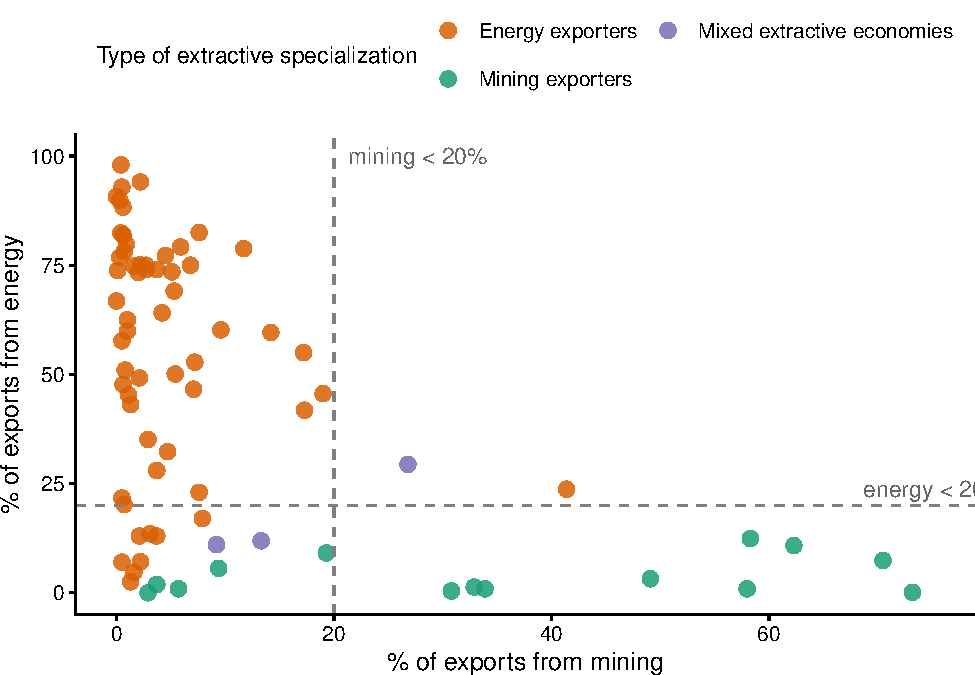
\includegraphics[width=\textwidth]{figures/extractive_specialization_scatter}
		
		\caption[Exportaciones mineras y energéticas]{Relación entre la participación de las exportaciones mineras y energéticas en la canasta exportadora de los países considerados. Las líneas punteadas indican umbrales del 20\% que permiten distinguir distintos patrones de especialización extractiva.}
		
		\label{fig:extractive-specialization}
	\end{figure}
	
	Un segundo patrón empírico surge al examinar la relación entre la dependencia exportadora de recursos extractivos y el nivel de ingreso de los países. La evidencia descriptiva sugiere que la dependencia de las exportaciones extractivas no disminuye de manera monotónica a medida que aumenta el ingreso per cápita (Figura \ref{fig:commodities-income}). Si bien las economías de bajos ingresos presentan una alta dispersión en su grado de dependencia, las economías de ingreso medio alto y varias economías de altos ingresos mantienen participaciones elevadas de recursos extractivos dentro de su estructura exportadora. En particular, la mediana de la participación de commodities en las exportaciones totales se mantiene en niveles relativamente altos para los grupos de ingreso medio alto y alto. Este patrón sugiere que la especialización en recursos naturales no necesariamente desaparece en etapas avanzadas del desarrollo económico, sino que puede coexistir con altos niveles de ingreso cuando la explotación de dichos recursos se articula con capacidades tecnológicas, institucionales y productivas más sofisticadas.
	
	\begin{figure}[H]
		\centering
		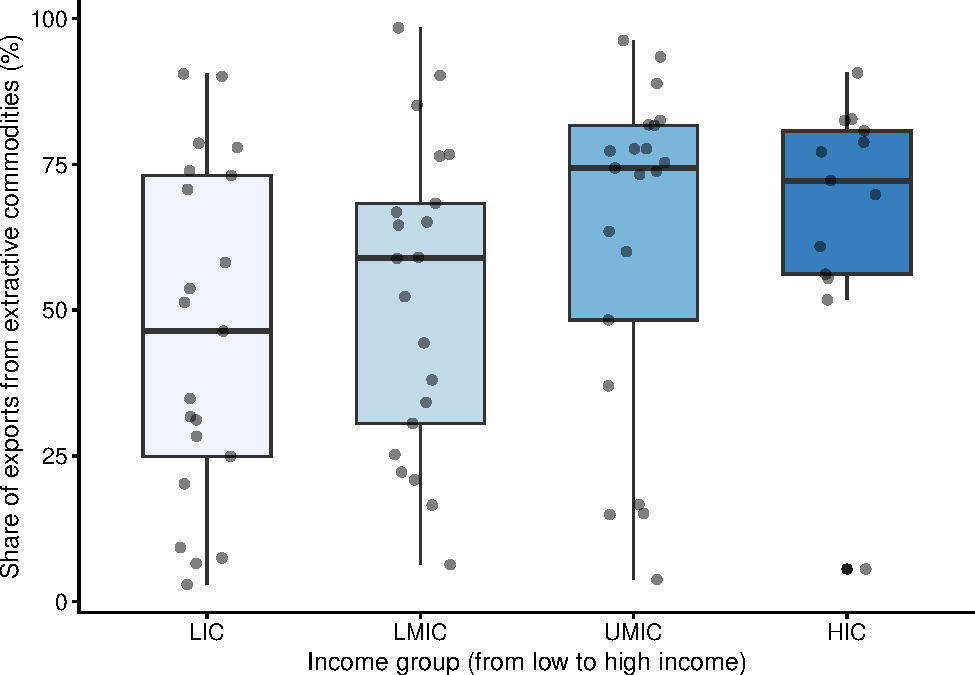
\includegraphics[width=\textwidth]{figures/p_commodities_income_boxplot}
		
		\caption[Dependencia exportadora de commodities por nivel de ingreso]{Distribución de la participación de las exportaciones de commodities en el total de exportaciones según grupo de ingreso: bajos ingresos (LIC), ingresos medios bajos (LMIC), ingresos medios altos (UMIC) y altos ingresos (HIC).}
		
		\label{fig:commodities-income}
	\end{figure}
	
	Un tercer patrón emerge al comparar la intensidad de la dependencia exportadora entre distintos tipos de recursos extractivos. Los resultados muestran que las economías especializadas en recursos energéticos presentan niveles sustancialmente más altos de concentración exportadora que aquellas especializadas en minería (Figuras \ref{fig:energy-income-boxplot} y \ref{fig:mining-income-boxplot}). Mientras que las exportaciones energéticas pueden llegar a representar una fracción dominante de la canasta exportadora en numerosos países, la participación de las exportaciones mineras tiende a ser considerablemente menor y más dispersa entre los distintos grupos de ingreso. En otras palabras, las economías petroleras exhiben estructuras exportadoras mucho más concentradas que las economías mineras. Este contraste sugiere que los distintos tipos de recursos naturales generan patrones de especialización económica diferenciados, lo que implica que las economías basadas en hidrocarburos pueden enfrentar dinámicas macroeconómicas y de diversificación productiva distintas a aquellas asociadas a la minería.
	
	\begin{figure}[H]
		\centering
		
		\begin{subfigure}{0.49\textwidth}
			\centering
			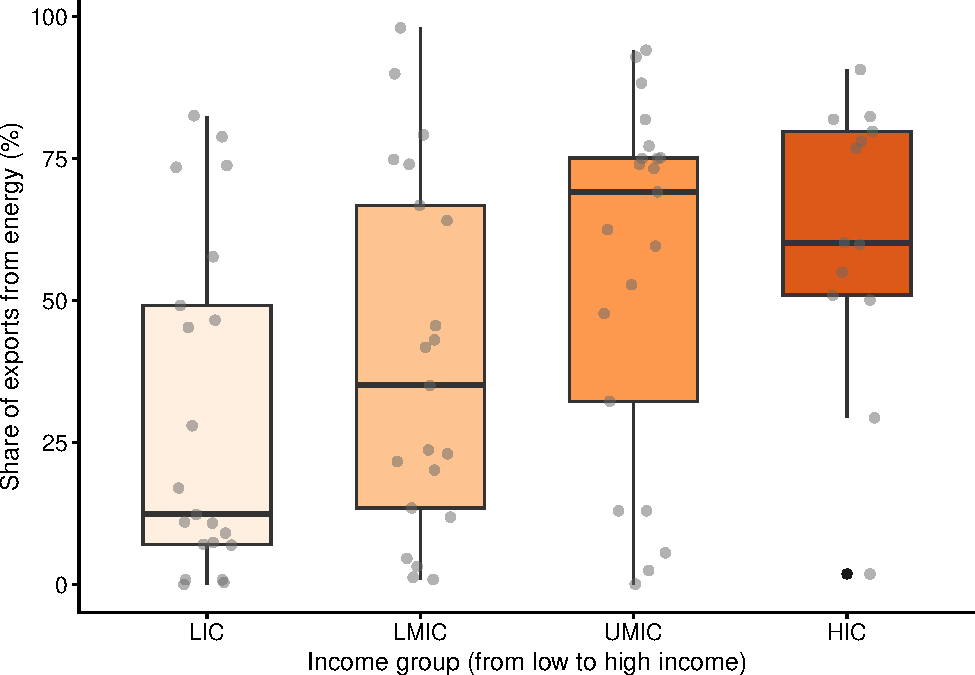
\includegraphics[width=\textwidth]{figures/p_energy_income_boxplot}
			\caption{Dependencia de exportaciones energéticas por grupo de ingreso.}
			\label{fig:energy-income-boxplot}
		\end{subfigure}
		\hfill
		\begin{subfigure}{0.49\textwidth}
			\centering
			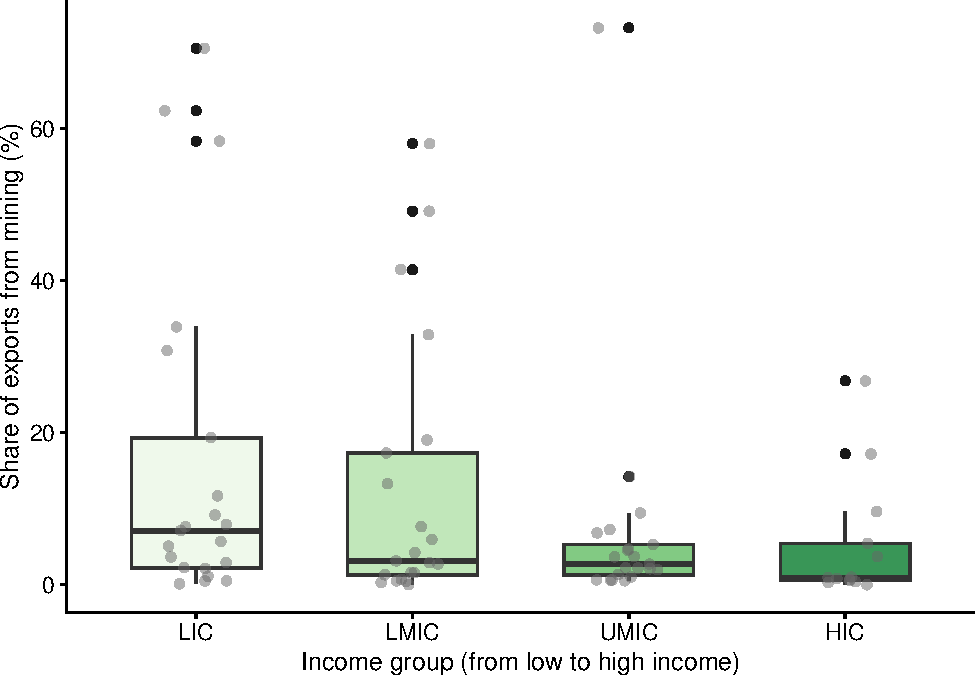
\includegraphics[width=\textwidth]{figures/p_mining_income_boxplot}
			\caption{Dependencia de exportaciones mineras por grupo de ingreso.}
			\label{fig:mining-income-boxplot}
		\end{subfigure}
		
		\caption[Dependencia exportadora por tipo de recurso]{Comparación de la participación de las exportaciones de recursos energéticos y mineros en el total de exportaciones de los países considerados.}
		
		\label{fig:energy-mining-income-comparison}
		
	\end{figure}
	
		\section{Análisis exploratorio de datos}
	\label{sec:análisis-exploratorio}
	
	La \autoref{fig:eci-vs-resource-rents-trim} muestra la relación entre el Índice de Complejidad Económica (ECI) y la dependencia de recursos naturales, medida como las rentas de recursos naturales como porcentaje del PIB. El gráfico presenta la distribución de países en función de ambos indicadores e incluye una estimación lineal por mínimos cuadrados ordinarios (OLS) y una curva de suavizamiento local (LOESS) que permiten identificar la tendencia general de la relación. En términos generales, se observa una asociación negativa entre la dependencia de recursos naturales y la complejidad económica, donde economías con mayores niveles de rentas provenientes de recursos tienden a presentar menores valores de ECI.
	
	
	\begin{figure}[H]
		\centering
		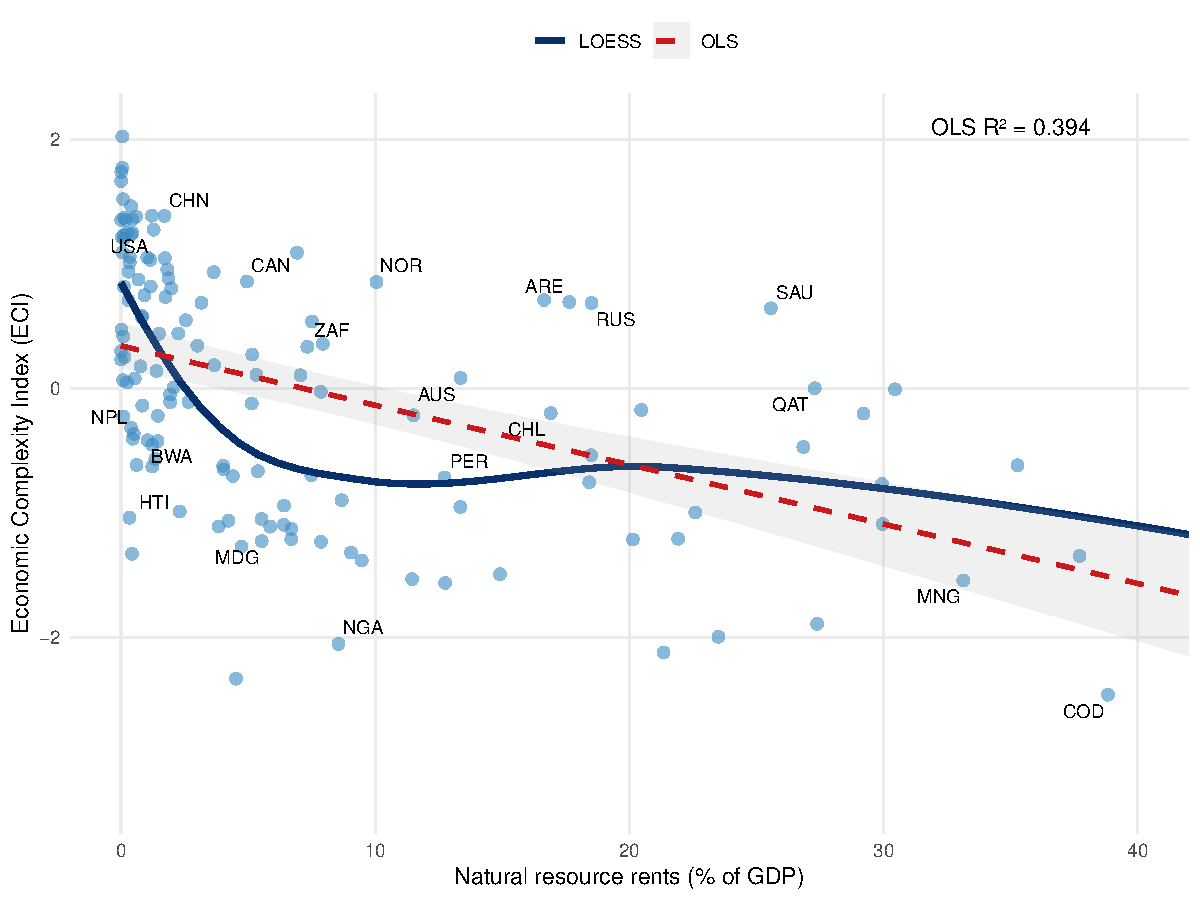
\includegraphics[width=\textwidth]{figures/eci_vs_resource_rents_trim}
		
		\caption[ECI y rentas de recursos naturales]{Relación entre el Índice de Complejidad Económica (ECI) y las rentas de recursos naturales como porcentaje del PIB.}
		
		\label{fig:eci-vs-resource-rents-trim}
	\end{figure}
	
	La \autoref{fig:eci-vs-rents-log-quad} presenta la relación entre el Índice de Complejidad Económica (ECI) y la dependencia de recursos naturales, medida como las rentas de recursos naturales como porcentaje del PIB, utilizando una escala logarítmica para facilitar la visualización de la distribución de países en niveles bajos de rentas donde se concentra una parte importante de la muestra. El gráfico incluye una estimación lineal por mínimos cuadrados ordinarios (OLS) y una curva de suavizamiento local (LOESS), lo que permite identificar la tendencia general y posibles patrones no lineales en la relación entre complejidad económica y dependencia de recursos; adicionalmente, las líneas punteadas dividen el espacio en cuadrantes que facilitan la comparación entre economías con distintos niveles de complejidad productiva y especialización en recursos naturales.
	
	\begin{figure}[H]
		\centering
		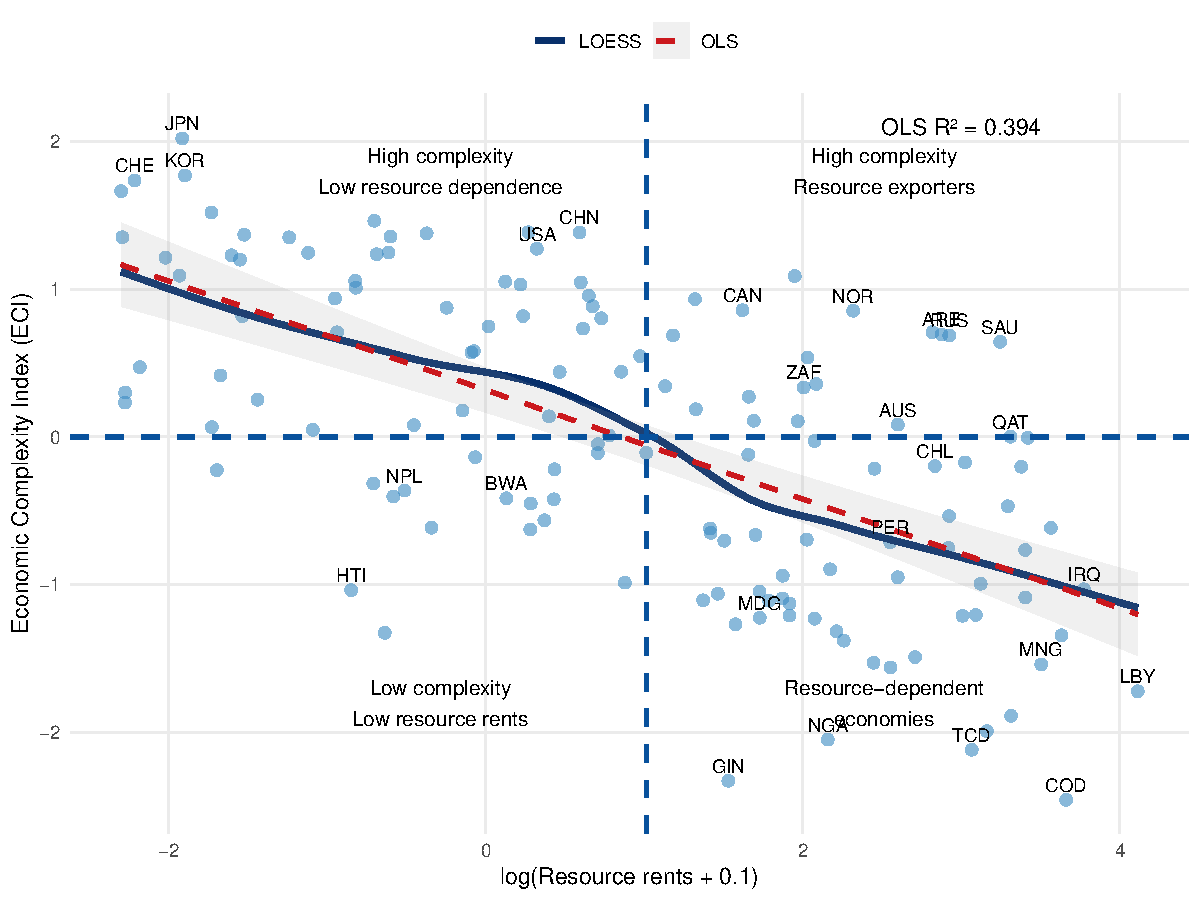
\includegraphics[width=\textwidth]{figures/eci_vs_rents_log_quad}
		
		\caption[ECI y rentas de recursos (escala log)]{Relación entre el Índice de Complejidad Económica (ECI) y las rentas de recursos naturales como porcentaje del PIB en escala logarítmica.}
		
		\label{fig:eci-vs-rents-log-quad}
	\end{figure}
	
	La \autoref{fig:rents-density} muestra la distribución de las rentas de recursos naturales como porcentaje del PIB para el conjunto de países analizados. La densidad evidencia una fuerte asimetría hacia la derecha, indicando que la mayoría de las economías presentan niveles relativamente bajos de dependencia de recursos, mientras que un grupo reducido de países exhibe valores considerablemente más altos. La figura también señala la media y la mediana de la distribución, lo que permite apreciar la diferencia entre ambas medidas y resaltar la presencia de observaciones con altos niveles de rentas provenientes de recursos naturales.
	
	\begin{figure}[H]
		\centering
		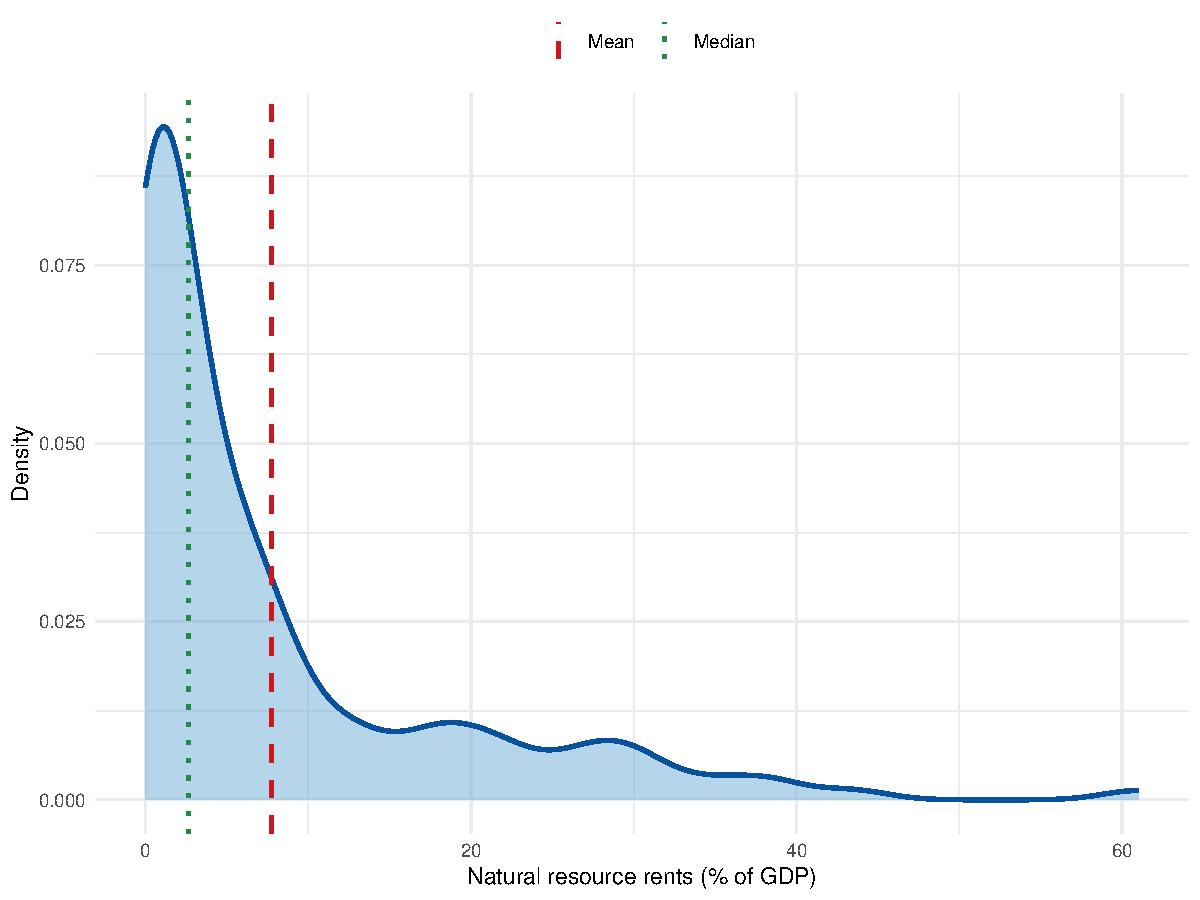
\includegraphics[width=\textwidth]{figures/rents_density}
		
		\caption[Distribución de rentas de recursos naturales (\% del PIB)]{Distribución de las rentas de recursos naturales como porcentaje del PIB.}
		
		\label{fig:rents-density}
	\end{figure}
	
	\thesisendchap{datos-variables}
	% =====================================================
	% RESULTADOS / HALLAZGOS / DESARROLLO
	% =====================================================
	\chapter{Resultados}
	\label{chap:resultados}
	\thesisstartchap{resultados}
	
	\section{Resultados principales}
	\label{sec:resultados-principales}
	

	\section{Análisis de robustez}
	\label{sec:robustez}
	
	
	\section{Discusión de resultados}
	\label{sec:discusion-resultados}
	
	
	
	\subsection{Ranking de capacidad de diversificación en economías dependientes de recursos naturales}
	\label{sec:ranking}
	
	Con el fin de complementar el análisis econométrico, se propone un ejercicio descriptivo orientado a comparar la posición relativa de las economías dependientes de recursos naturales en términos de su capacidad de diversificación productiva. A diferencia de enfoques que miden la transformación estructural a partir del crecimiento del sector no extractivo, este trabajo utiliza el \textit{Economic Complexity Index} (ECI) como una medida sintética de las capacidades productivas subyacentes.
	
	La lógica de este enfoque se basa en la literatura de complejidad económica, según la cual la diversificación no debe entenderse únicamente como la expansión de sectores no extractivos, sino como la acumulación de capacidades que permiten a una economía producir y exportar bienes más diversos y sofisticados. En este sentido, el ECI captura de manera indirecta el grado de diversificación efectiva de la estructura productiva, penalizando la dependencia en productos primarios y reflejando la proximidad hacia actividades de mayor complejidad.
	
	En consecuencia, el ejercicio propuesto considera dos dimensiones complementarias de la diversificación: (i) el nivel de complejidad económica, que refleja el estado actual de las capacidades productivas, y (ii) la dinámica de la complejidad, que captura la evolución de dichas capacidades en el tiempo.
	
	Formalmente, se definen:
	
	\begin{equation}
		RTC_i^{nivel} = ECI_i
	\end{equation}
	
	\begin{equation}
		RTC_i^{din} = \Delta ECI_i = ECI_{i,t} - ECI_{i,t-k}
	\end{equation}
	
	donde $RTC_i^{nivel}$ representa la capacidad de diversificación en términos de la estructura productiva actual, mientras que $RTC_i^{din}$ captura el cambio en dicha capacidad a lo largo del tiempo.
	
	Esta distinción permite diferenciar entre economías que ya poseen estructuras productivas complejas y aquellas que, aun partiendo de niveles bajos de complejidad, muestran procesos de transformación estructural dinámicos. En particular, el análisis conjunto de ambas dimensiones permite identificar trayectorias diferenciadas de desarrollo productivo dentro del grupo de economías dependientes de recursos naturales.
	
	De este modo, el ranking no solo ordena a los países según su nivel de complejidad económica, sino que también permite clasificar su desempeño en términos de transición estructural, distinguiendo entre economías consolidadas, economías en proceso de diversificación y economías con persistente dependencia de recursos naturales.
	
	Finalmente, este enfoque permite identificar heterogeneidad significativa entre economías con similares niveles de dependencia de recursos, evidenciando que dicha dependencia no determina de manera unívoca la capacidad de diversificación productiva. Por el contrario, algunos países logran desarrollar estructuras productivas más complejas o avanzar dinámicamente hacia ellas, lo que sugiere la existencia de factores adicionales —institucionales, educativos y tecnológicos— que condicionan las trayectorias de transformación estructural.
	
	\thesisendchap{resultados}
	
	% =====================================================
	% CONCLUSIONES
	% =====================================================
	\chapter{Conclusiones}
	\label{chap:conclusiones}
	
	\thesisstartchap{conclusiones}
	
	
	\thesisendchap{conclusiones}
	
	
	% =====================================================
	% CRONOGRAMA
	% =====================================================
	
	\chapter*{Planificación de la tesis}
	\label{chap:planificación}
	
	La \autoref{tab:cronograma} resume el cronograma tentativo de las actividades previstas para el desarrollo del trabajo durante el año 2026, en coherencia con las etapas metodológicas descritas en el \autoref{chap:metodología}.
	
	\begin{longtable}{|p{6.2cm}|*{12}{c|}}
		\caption[Cronograma de actividades]{Cronograma tentativo de las actividades de investigación durante el año 2026.}
		
		\label{tab:cronograma} \\
		\hline
		\textbf{Actividad} & \multicolumn{12}{c|}{\textbf{Meses del año 2026}} \\
		\hline
		& 1 & 2 & 3 & 4 & 5 & 6 & 7 & 8 & 9 & 10 & 11 & 12 \\
		\hline
		\endfirsthead
		
		\multicolumn{13}{c}%
		{{\tablename\ \thetable{} -- continuación}} \\
		\hline
		\textbf{Actividad} & \multicolumn{12}{c|}{\textbf{Meses del año 2026}} \\
		\hline
		& 1 & 2 & 3 & 4 & 5 & 6 & 7 & 8 & 9 & 10 & 11 & 12 \\
		\hline
		\endhead
		
		\hline
		\multicolumn{13}{r}{\textit{Continúa en la página siguiente}} \\
		\endfoot
		
		\hline
		\endlastfoot
		
		\textbf{1.} Revisión exploratoria de literatura y organización bibliográfica (artículos académicos, Mendeley)
		& \cellcolor{gray!40} & \cellcolor{gray!40} &  &  &  &  &  &  &  &  &  &  \\
		\cline{2-13}
		
		\textbf{2.} Ajustes del marco teórico y revisión dirigida de literatura
		&  & \cellcolor{gray!40} & \cellcolor{gray!40} & \cellcolor{gray!40} &  &  &  &  &  &  &  &  \\
		\cline{2-13}
		
		\textbf{3.} Construcción, extracción y limpieza de la base de datos
		&  & \cellcolor{gray!40} & \cellcolor{gray!40} & \cellcolor{gray!40} &  &  &  &  &  &  &  &  \\
		\cline{2-13}
		
		\textbf{4.} Especificación formal del modelo econométrico y definición final de variables
		&  &  & \cellcolor{gray!40} & \cellcolor{gray!40} &  &  &  &  &  &  &  &  \\
		\cline{2-13}
		
		\textbf{5.} Análisis descriptivo y caracterización de trayectorias
		&  &  & \cellcolor{gray!40} & \cellcolor{gray!40} & \cellcolor{gray!40} &  &  &  &  &  &  &  \\
		\cline{2-13}
		
		\textbf{6.} Estimaciones econométricas y pruebas de robustez
		&  &  &  & \cellcolor{gray!40} & \cellcolor{gray!40} & \cellcolor{gray!40} &  &  &  &  &  &  \\
		\cline{2-13}
		
		\textbf{7.} Análisis de resultados e integración con el marco analítico
		&  &  &  &  &  & \cellcolor{gray!40} & \cellcolor{gray!40} &  &  &  &  &  \\
		\cline{2-13}
		
		\textbf{8.} Redacción de resultados
		&  &  &  &  &  & \cellcolor{gray!40} & \cellcolor{gray!40} & \cellcolor{gray!40} &  &  &  &  \\
		\cline{2-13}
		
		\textbf{9.} Redacción de conclusiones y recomendaciones
		&  &  &  &  &  &  &  & \cellcolor{gray!40} & \cellcolor{gray!40} &  &  &  \\
		\cline{2-13}
		
		\textbf{10.} Correcciones finales, revisión integral y entrega
		&  &  &  &  &  &  &  &  & \cellcolor{gray!40} & \cellcolor{gray!40} & \cellcolor{gray!40} &  \\
		
		\hline
		\multicolumn{13}{p{\textwidth}}{%
			\textit{Nota: El cronograma es tentativo y puede ajustarse según el avance del trabajo y la disponibilidad de información.}
		} 
		
	\end{longtable}
	
	\begin{table}[H]
		\centering
		
		\caption[Extensión sugerida de los capítulos]{Distribución sugerida de la extensión de los capítulos de la tesis.}
		
		\label{tab:estructura_longitud_tesis}
		
		\begin{threeparttable}
			
			\resizebox{\textwidth}{!}{
				\begin{tabular}{lccc}
					\toprule
					\textbf{Capítulo} & \textbf{Páginas aproximadas} & \textbf{Porcentaje estimado} & \textbf{Páginas actuales} \\
					\midrule
					
					Introducción \ref{chap:introducción} & 10--12 & 8--10\% & \thesischappages{introducción} \\
					Pregunta de investigación \ref{chap:pregunta} & 2--3 & 2--3\% & \thesischappages{pregunta} \\
					Justificación \ref{chap:justificación} & 3--4 & 2--3\% & \thesischappages{justificación} \\
					Planteamiento del problema \ref{chap:planteamiento} & 3--4 & 2--3\% & \thesischappages{planteamiento} \\
					Objetivos \ref{chap:objetivos} & 1--2 & 1--2\% & \thesischappages{objetivos} \\
					Hipótesis \ref{chap:hipótesis} & 2--3 & 2--3\% & \thesischappages{hipótesis} \\
					
					Marco teórico \ref{chap:marco-teórico} & 18--20 & 14--16\% & \thesischappages{marco-teórico} \\
					Literatura empírica \ref{chap:literatura-empírica} & 10--12 & 8--10\% & \thesischappages{literatura-empírica} \\
					
					Metodología \ref{chap:metodología} & 8--10 & 6--8\% & \thesischappages{metodología} \\
					Datos y construcción de variables \ref{chap:datos-variables} & 5--6 & 4--5\% & \thesischappages{datos-variables} \\
					
					Resultados \ref{chap:resultados} & 35--40 & 28--32\% & \thesischappages{resultados} \\
					Conclusiones \ref{chap:conclusiones} & 6--8 & 5--7\% & \thesischappages{conclusiones} \\
					
					Anexos \ref{chap:anexos} & 15--20 & 12--15\% & \thesischappages{anexos} \\
					
					\midrule
					\textbf{Total aproximado} & \textbf{120--125} & \textbf{100\%} & \textbf{\pageref{LastPage}} \\
					
					\bottomrule
				\end{tabular}
			}
			
			\begin{tablenotes}
				\small
				\item \textit{Nota: La tabla presenta una distribución referencial de la extensión de los capítulos para una tesis de aproximadamente 120--125 páginas.}
			\end{tablenotes}
			
		\end{threeparttable}
		
	\end{table}
	
	% =====================================================
	% REFERENCIAS BIBLIOGRÁFICAS
	% =====================================================
	\printbibliography
	
	% =====================================================
	% ANEXOS
	% =====================================================
	\appendix
	\chapter{Anexos}
	\label{chap:anexos}
	\thesisstartchap{anexos}
	
	\section{Fuentes preliminares de datos e indicadores}
	\label{sec:fuentes}
	
	La \autoref{tab:fuentes_datos} presenta, de manera preliminar, posibles indicadores empíricos y posibles fuentes internacionales de datos. La selección definitiva de variables se realizará en la etapa de implementación empírica, atendiendo a criterios de disponibilidad, comparabilidad y consistencia teórica.
	
	\renewcommand{\arraystretch}{1.2}
	\setlength{\tabcolsep}{4pt}
	
	\begin{small}
		\begin{longtable}{
				p{2.6cm}
				p{3.0cm}
				p{4.2cm}
				p{3.6cm}
				p{1.8cm}
			}
			
			\caption[Fuentes de datos para el panel empírico]{Fuentes de datos utilizadas para la construcción del panel empírico.}
			
			\label{tab:fuentes_datos} \\
			\hline
			\textbf{Dimensión} & \textbf{Variable conceptual} & \textbf{Indicador utilizado} & \textbf{Fuente internacional} & \textbf{Cobertura} \\
			\hline
			\endfirsthead
			
			\hline
			\textbf{Dimensión} & \textbf{Variable conceptual} & \textbf{Indicador utilizado} & \textbf{Fuente internacional} & \textbf{Cobertura} \\
			\hline
			\endhead
			
			Dependencia extractiva
			& Dependencia de recursos (principal)
			& Rentas de recursos naturales (\% del PIB) (RES\_RENT)
			& World Bank (WDI)
			& 1970--2022 \\
			
			Dependencia extractiva
			& Dependencia de recursos (alternativa)
			& Exportaciones de recursos / exportaciones totales (RES\_EXP)
			& UN Comtrade; World Bank
			& 1980--2022 \\
			
			Estructura productiva
			& Complejidad económica
			& Índice de Complejidad Económica (ECI, HS92)
			& Atlas of Economic Complexity
			& 1995--2022 \\
			
			Estructura productiva
			& Concentración exportadora
			& Índice de Herfindahl--Hirschman (HHI)
			& UN Comtrade; Atlas of Economic Complexity
			& 1980--2022 \\
			
			Instituciones
			& Calidad institucional
			& Rule of Law; Control of Corruption (INST)
			& Worldwide Governance Indicators (WGI)
			& 1996--2022 \\
			
			Capacidades productivas
			& Capital humano
			& Años promedio de escolaridad (HUMCAP)
			& Barro--Lee; World Bank
			& 1950--2020 \\
			
			Capacidades productivas
			& Innovación
			& Gasto en I+D (\% del PIB) o patentes (INNOV)
			& UNESCO; WIPO
			& 1996--2022 \\
			
			Macroeconomía
			& Volatilidad externa
			& Volatilidad de precios de commodities (VOL\_TOT)
			& World Bank (Pink Sheet)
			& 1960--2022 \\
			
			Macroeconomía
			& Tipo de cambio real
			& Tipo de cambio real efectivo (RER)
			& World Bank; BIS; IMF
			& 1980--2022 \\
			
			Control
			& Nivel de desarrollo
			& PIB per cápita (PPA, log) (GDPPC)
			& World Bank (WDI)
			& 1980--2022 \\
			
			Canal financiero
			& Política fiscal
			& Balance fiscal / deuda (\% del PIB) (FISC)
			& IMF; World Bank
			& 1980--2022 \\
			
			Canal financiero
			& Desarrollo financiero
			& Crédito doméstico al sector privado (\% PIB) (FIN)
			& World Bank (WDI)
			& 1980--2022 \\
			
			\hline
			\multicolumn{5}{p{14.5cm}}{\textit{Nota: El panel se construye con frecuencia anual. La variable principal de complejidad corresponde al ECI basado en clasificación HS92 para asegurar consistencia temporal. Las variables de dependencia de recursos se incorporan de forma alternativa en las estimaciones para evitar problemas de multicolinealidad. La muestra final es un panel desbalanceado determinado por la disponibilidad de datos.}} \\
		\end{longtable}
	\end{small}
	
	\section{Figuras conceptuales y esquemas analíticos}
	\label{sec:figuras}
	
	Esta sección reúne las figuras conceptuales y esquemas analíticos que apoyan la exposición teórica y metodológica del trabajo. Los diagramas permiten visualizar de forma sintética algunos de los mecanismos de transición estructural y  relaciones entre las principales variables analizadas, facilitando la interpretación del enfoque general del estudio.
	
	\begin{figure}[H]
		\centering
		\resizebox{\linewidth}{!}{%
			\begin{tikzpicture}[
				font=\small,
				node distance=1.55cm and 2.9cm,
				box/.style={
					draw,
					rectangle,
					rounded corners=6pt,
					align=center,
					minimum width=6.0cm,
					minimum height=1.05cm,
					inner sep=6pt
				},
				sidebox/.style={
					draw,
					rectangle,
					rounded corners=6pt,
					align=center,
					minimum width=4.3cm,
					minimum height=0.95cm,
					inner sep=6pt
				},
				arrow/.style={-{Stealth[length=3mm]}, line width=0.7pt}
				]
				
				% Columna central
				\node[box] (res) {Dependencia de recursos\\[2pt]\textit{(RES)}};
				
				\node[box, below=of res] (canales) {Canales productivos\\
					Enfermedad holandesa\\
					Enclaves productivos\\
					Tipo de cambio real};
				
				\node[box, below=1.9cm of canales] (resultados) {Resultados productivos\\
					Diversificación\\
					Innovación\\
					Acumulación de capacidades};
				
				% Laterales
				\node[sidebox, left=of canales] (inst) {Instituciones\\[2pt]\textit{(INST)}};
				\node[sidebox, right=of canales] (vol) {Volatilidad externa\\[2pt]\textit{(VOL)}};
				\node[sidebox, right=of resultados] (fisc) {Restricción fiscal\\[2pt]\textit{(FISC)}};
				
				% Flechas
				\draw[arrow] (res) -- (canales);
				\draw[arrow] (canales) -- (resultados);
				
				\draw[arrow] (inst) -- node[above, font=\small] {modula} (canales);
				\draw[arrow] (vol) -- node[above, font=\small] {condiciona} (canales);
				\draw[arrow] (fisc) -- node[above, font=\small] {limita} (resultados);
				
			\end{tikzpicture}%
		}
		
		\caption[Arquitectura conceptual de la transición estructural]{Arquitectura conceptual de los mecanismos que vinculan la dependencia de recursos naturales con los resultados de diversificación, innovación y acumulación de capacidades.}
		
		\label{fig:arquitectura-mecanismos}
	\end{figure}
	
	Con el fin de evaluar la robustez de los resultados y considerar dimensiones adicionales de la transformación estructural no capturadas por el \textit{Economic Complexity Index (ECI)}, se estiman especificaciones alternativas en las que la variable dependiente corresponde a indicadores de la estructura productiva interna. En particular, se utilizan \textit{Manufacturing Value Added (MANVA)} y \textit{Services Value Added (SERVVA)} como proporción del PIB, como aproximaciones a la composición sectorial de la economía. Estas variables permiten capturar procesos de diversificación productiva que tienen lugar en el ámbito doméstico, complementando así el análisis basado en la sofisticación de la estructura exportadora. De este modo, se contrasta si los efectos de la dependencia de recursos naturales y los demás determinantes del modelo se mantienen al analizar la transformación estructural desde una perspectiva interna.
	
	\begin{figure}[H]
		\centering
		\begin{tikzpicture}[
			font=\normalsize,
			box/.style={
				draw,
				rounded corners=3pt,
				align=center,
				minimum width=0.65\textwidth,
				minimum height=10mm,
				inner ysep=6pt
			},
			arr/.style={-{Stealth[length=3mm]}, thick},
			node distance=7mm
			]
			
			\node[box] (a) {Boom de commodities};
			\node[box, below=of a] (b) {expansi\'on fiscal};
			\node[box, below=of b] (c) {apreciaci\'on};
			\node[box, below=of c] (d) {desplazamiento\\manufacturero};
			\node[box, below=of d] (e) {ajuste post-boom};
			
			\draw[arr] (a) -- (b);
			\draw[arr] (b) -- (c);
			\draw[arr] (c) -- (d);
			\draw[arr] (d) -- (e);
			
		\end{tikzpicture}
		\caption[Mecanismo boom y ajuste post-boom]{Esquema conceptual del mecanismo de boom de commodities y el proceso de ajuste posterior en la estructura productiva.}
		
		\label{fig:esquema_boom_postboom_vertical}
	\end{figure}
	
	\begin{figure}[H]
		\centering
		\begin{tikzpicture}[
			font=\normalsize,
			box/.style={
				draw,
				rounded corners=3pt,
				align=center,
				minimum width=0.72\textwidth,
				minimum height=10mm,
				inner ysep=6pt
			},
			arr/.style={-{Stealth[length=3mm]}, thick},
			node distance=7mm
			]
			
			\node[box] (s1) {Fuentes internacionales};
			\node[box, below=of s1] (s2) {Construcci\'on de base panel};
			\node[box, below=of s2] (s3) {Limpieza y armonizaci\'on};
			\node[box, below=of s3] (s4) {Modelo econom\'etrico};
			\node[box, below=of s4] (s5) {Resultados};
			
			\draw[arr] (s1) -- (s2);
			\draw[arr] (s2) -- (s3);
			\draw[arr] (s3) -- (s4);
			\draw[arr] (s4) -- (s5);
			
		\end{tikzpicture}
		
		\caption[Construcción del panel de datos]{Diagrama metodológico del proceso de construcción del panel de datos utilizado en el análisis empírico.}
		
		\label{fig:diagrama_panel}
	\end{figure}
	
	La evolución del debate sobre la denominada “maldición de los recursos” puede entenderse como una transición desde interpretaciones clásicas
	que consideraban los recursos naturales como una ventaja para el desarrollo, hasta enfoques contemporáneos que analizan los mecanismos institucionales,
	macroeconómicos y estructurales que pueden convertir dicha abundancia en un factor limitante del crecimiento económico. La \autoref{fig:resource_curse_timeline} sintetiza esta evolución conceptual.
	
	\begin{figure}[H]
		\centering
		\resizebox{\textwidth}{!}{
			\begin{tikzpicture}[
				box/.style={
					rectangle,
					rounded corners,
					draw=black,
					thick,
					text width=3.5cm,
					minimum height=2.6cm,
					text centered,
					align=center,
					fill=gray!10,
					font=\small
				}
				]
				
				% Timeline
				\draw[thick] (-1,-2) -- (24,-2);
				
				% Top boxes
				\node[box] at (0,0)
				{Los recursos naturales\\ tienen un papel positivo\\ en el desarrollo económico};
				
				\node[box] at (4.8,0)
				{Surgimiento de la teoría\\ de la enfermedad holandesa};
				
				\node[box] at (9.6,0)
				{Formulación de la tesis\\ de la maldición de los\\ recursos (estudios de caso)};
				
				\node[box] at (14.4,0)
				{Se acuña el término\\ ``maldición de los\\ recursos''};
				
				\node[box] at (19.2,0)
				{Evidencia empírica que\\ confirma los efectos\\ adversos de la dependencia\\ de recursos};
				
				\node[box] at (24,0)
				{Relación entre dependencia\\ de recursos y\\ crecimiento económico};
				
				% Vertical connectors
				\draw (0,-0.8) -- (0,-2);
				\draw (4.8,-0.8) -- (4.8,-2);
				\draw (9.6,-0.8) -- (9.6,-2);
				\draw (14.4,-0.8) -- (14.4,-2);
				\draw (19.2,-0.8) -- (19.2,-2);
				\draw (24,-0.8) -- (24,-2);
				
				% Years
				\node at (0,-2.7) {Antes de 1980};
				\node at (4.8,-2.7) {1982};
				\node at (9.6,-2.7) {1988};
				\node at (14.4,-2.7) {1993};
				\node at (19.2,-2.7) {1995};
				\node at (24,-2.7) {2001};
				
				% Authors (below years)
				\node at (0,-3.4) {\small Adam Smith (1776)};
				\node at (4.8,-3.4) {\small Corden \& Neary};
				\node at (9.6,-3.4) {\small Gelb};
				\node at (14.4,-3.4) {\small Auty};
				\node at (19.2,-3.4) {\small Sachs \& Warner};
				\node at (24,-3.4) {\small Gylfason};
				
			\end{tikzpicture}
		}
		
		\caption[Evolución de la literatura sobre la maldición de los recursos]{Evolución conceptual de la literatura sobre la maldición de los recursos naturales.}
		
		\label{fig:resource_curse_timeline}
		
		\footnotesize
		\textit{Nota:} La figura resume el desarrollo histórico del debate sobre recursos naturales y crecimiento económico, desde las primeras interpretaciones clásicas hasta la evidencia empírica moderna sobre dependencia de recursos y desempeño económico.
		
		\textit{Fuente:} Elaboración propia con base en \textcite{Anne2021}.
		
	\end{figure}
	
	
	\vspace{1cm}
	
	
	\begin{figure}[H]
		\centering
		\begin{tikzpicture}[
			node distance=0.95cm,
			box/.style={
				draw,
				rectangle,
				rounded corners=4pt,
				align=center,
				minimum width=6.5cm,
				minimum height=1.1cm,
				font=\small
			},
			arrow/.style={->, thick}
			]
			
			\node[box] (cap) {Capacidades productivas};
			\node[box, below=of cap] (ps) {\textit{Product space}};
			\node[box, below=of ps] (div) {Diversificación productiva};
			\node[box, below=of div] (eci) {Complejidad económica (ECI)};
			\node[box, below=of eci] (growth) {Crecimiento económico de largo plazo};
			
			\draw[arrow] (cap) -- (ps);
			\draw[arrow] (ps) -- (div);
			\draw[arrow] (div) -- (eci);
			\draw[arrow] (eci) -- (growth);
			
		\end{tikzpicture}
		
		\caption[Capacidades productivas y complejidad económica]{Relación conceptual entre capacidades productivas, diversificación y complejidad económica.}
		
		\label{fig:secuencia-complejidad}
	\end{figure}
	
	Como se ilustra en la Figura \ref{fig:ul-durar-2023}, la relación entre la complejidad económica y las rentas de recursos puede adoptar una forma de U invertida. En etapas tempranas del desarrollo, caracterizadas por bajos niveles de complejidad, un aumento en la sofisticación productiva puede estar asociado con una expansión de las rentas derivadas de recursos naturales, reflejando una mejor organización productiva y aprovechamiento de dichos recursos. Sin embargo, a partir de cierto umbral de complejidad, se observa un proceso de sustitución en el cual las economías tienden a diversificarse hacia actividades más sofisticadas, reduciendo gradualmente la dependencia relativa de las rentas de recursos. Este patrón es consistente con los hallazgos de \textcite{Ul-Durar2023}, quienes documentan una relación no lineal entre complejidad económica y dependencia de recursos.
	
	\begin{figure}[htbp]
		\centering
		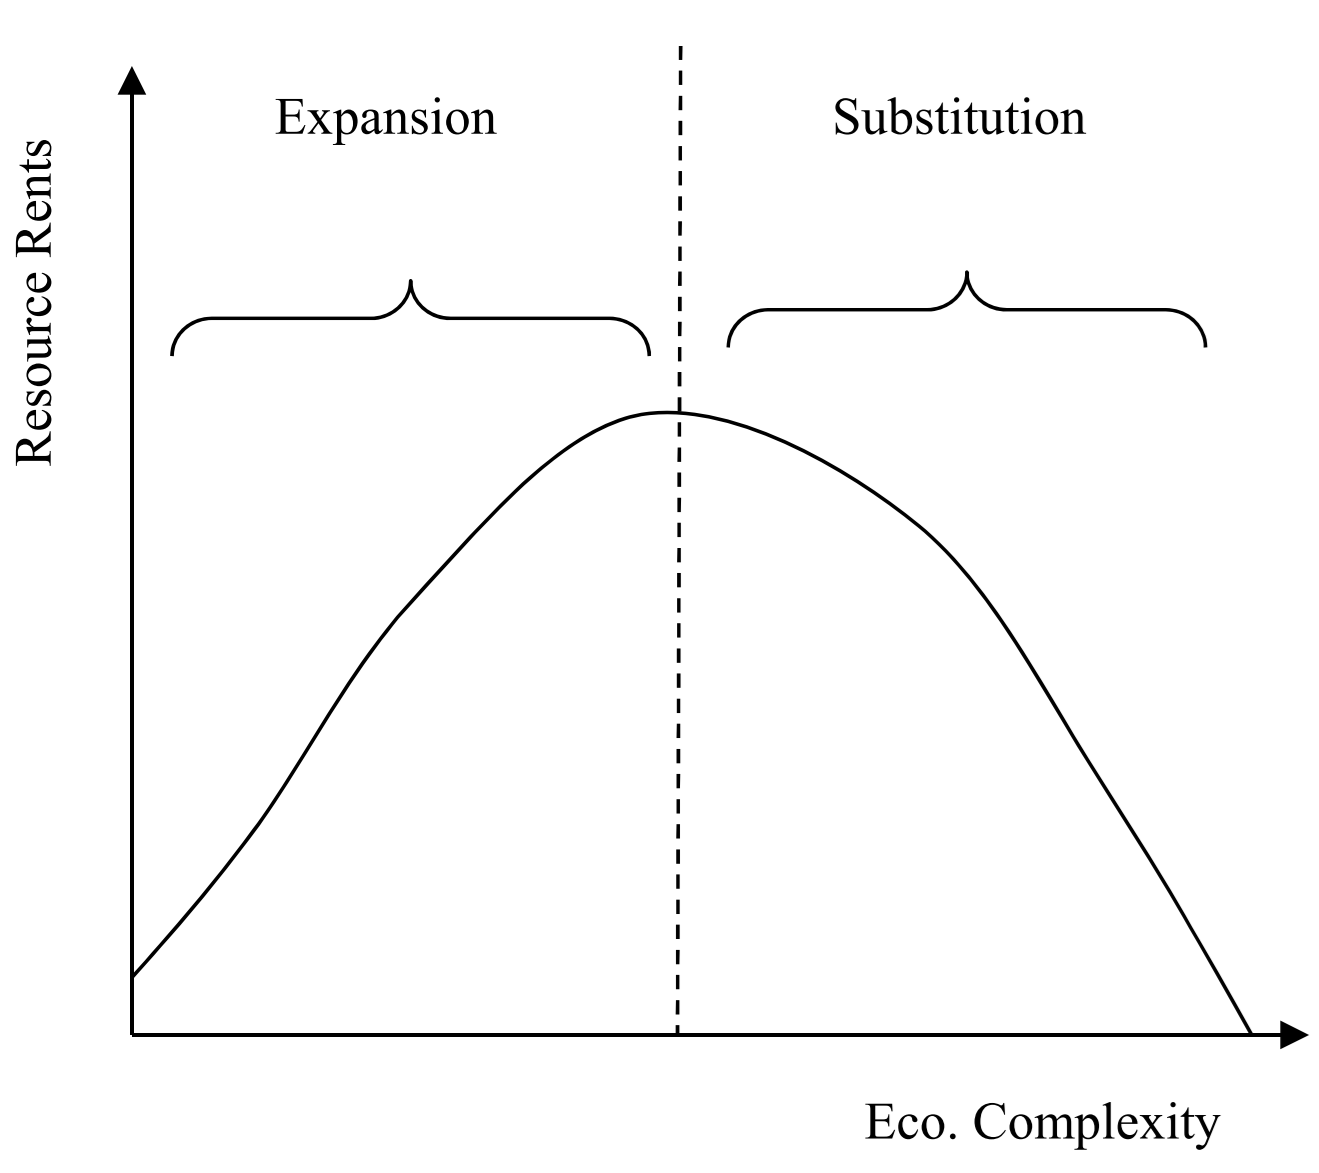
\includegraphics[width=0.8\textwidth]{figures/1_ul-durar_2023.png}
		\caption[Relación ECI y rentas de recursos (U invertida)]{
			Relación en forma de U invertida entre complejidad económica y rentas de recursos. Fuente: tomado de \textcite{Ul-Durar2023}.
		}
		\label{fig:ul-durar-2023}
	\end{figure}
	
	Por otra parte, la literatura también ha identificado una relación en forma de U, asociada al concepto de \textit{load capacity curve} (LCC), en la cual los incrementos iniciales en la complejidad económica reducen la dependencia de recursos a través de procesos de diversificación, pero en etapas avanzadas generan un efecto de escala que incrementa nuevamente la demanda por recursos naturales.
	
	\begin{figure}[htbp]
		\centering
		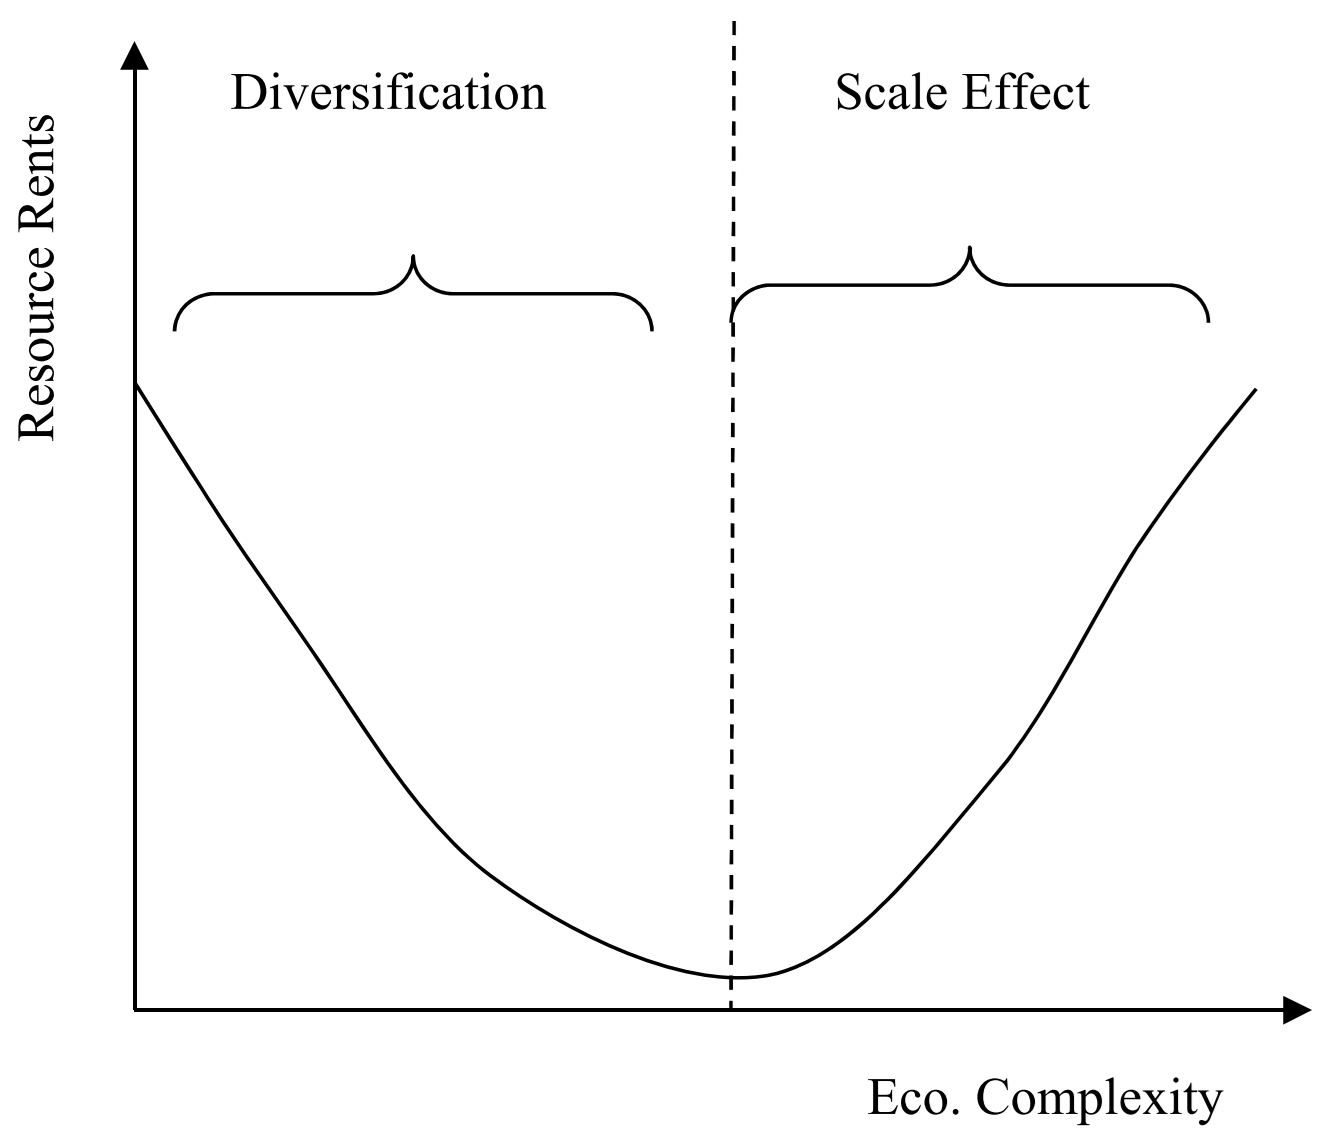
\includegraphics[width=0.8\textwidth]{figures/2_ul-durar_2023.png}
		\caption[Relación ECI y rentas de recursos (forma de U)]{
			Relación en forma de U entre complejidad económica y rentas de recursos: diversificación y efecto escala (\textit{load capacity curve}). Fuente: tomado de \textcite{Ul-Durar2023}.
		}
		\label{fig:ul-durar-u-shape}
	\end{figure}
	
	\section{Plots}
	\label{sec:plots}
	
		La \autoref{fig:eci_income_resources} muestra la relación entre el índice de complejidad económica (ECI) y el ingreso per cápita para 128 países. Los países se clasifican según su dependencia de recursos naturales: en rojo aquellos donde las exportaciones de recursos naturales representan más del 10\% del PIB y en azul aquellos con menor dependencia. Para el grupo de economías con baja presencia de recursos naturales, el ECI explica aproximadamente el 75\% de la variación en el ingreso per cápita entre países, lo que evidencia una fuerte relación entre complejidad productiva y nivel de desarrollo. En contraste, algunos países intensivos en recursos naturales presentan niveles de ingreso superiores a los que su complejidad productiva sugeriría, reflejando el efecto de las rentas derivadas de la explotación de petróleo, gas o minerales. No obstante, incluso dentro de este grupo la complejidad económica continúa mostrando una correlación positiva con el ingreso.
	
	
	\begin{figure}[H]
		\centering
		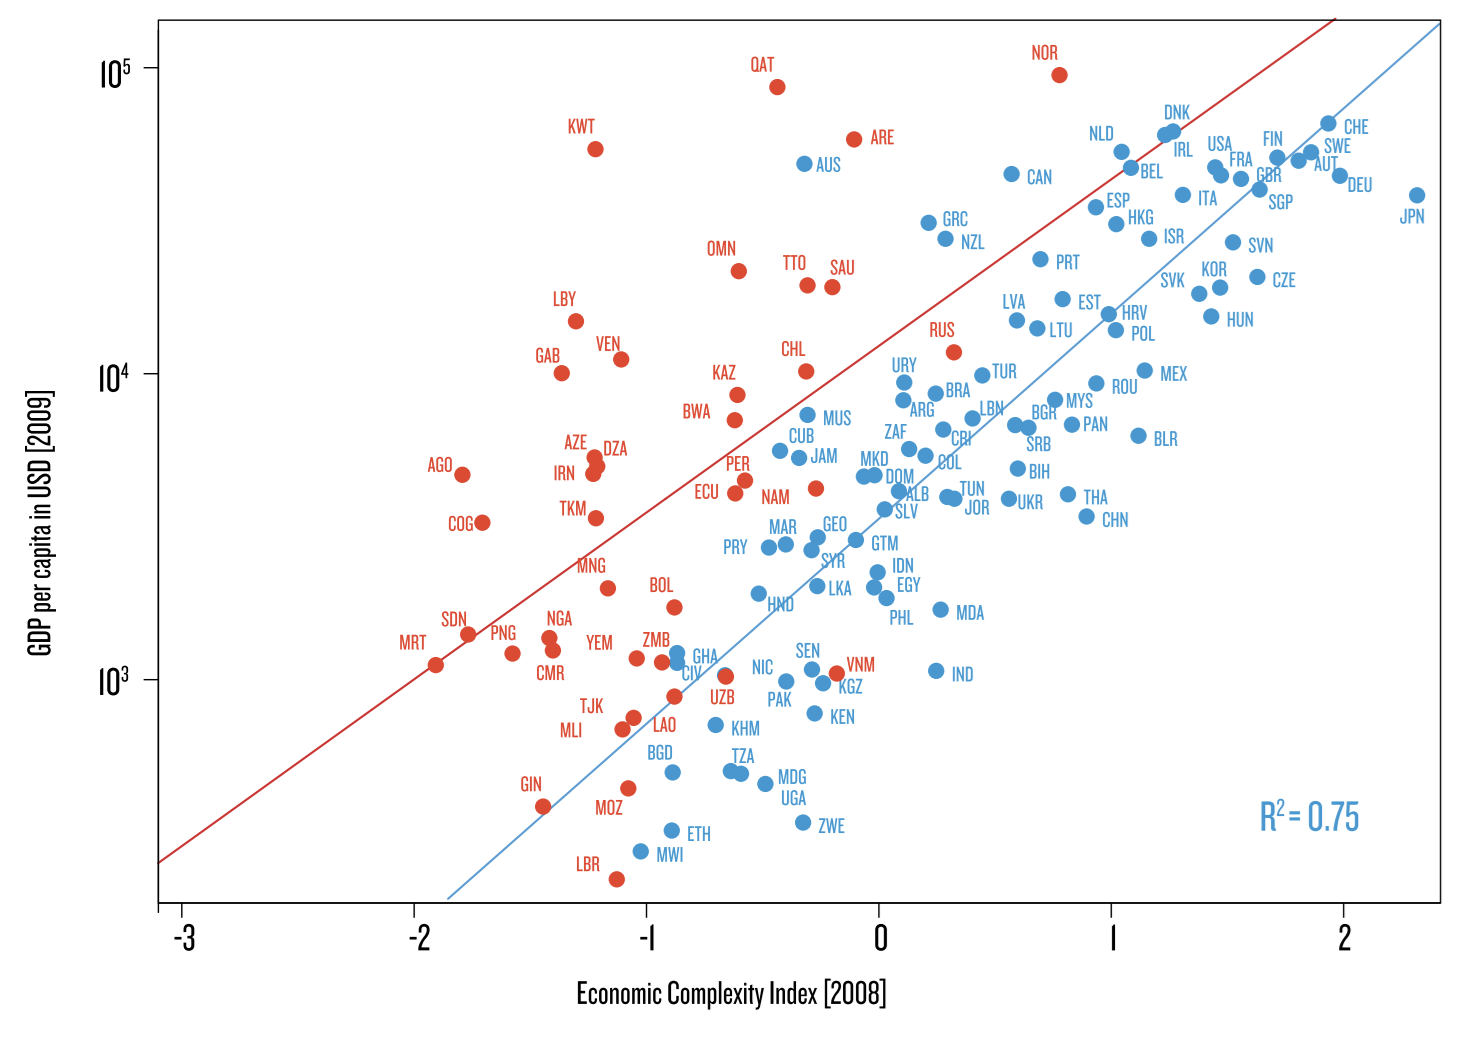
\includegraphics[width=0.9\textwidth]{figures/2_hausmann_2014.png}
		
		\caption[ECI e ingreso per cápita]{Relación entre el Índice de Complejidad Económica (ECI) y el ingreso per cápita para 128 países. Los colores distinguen economías dependientes de recursos naturales y economías con menor dependencia.}
		
		\label{fig:eci_income_resources}
		\caption*{\footnotesize \textit{Fuente: Tomado de \textcite{Hausmann2014}.}}
	\end{figure}
	
	La Figura~\ref{fig:anexo_nr_eci} muestra la relación entre la abundancia de recursos naturales y la complejidad económica. Se observa una asociación negativa en promedio, aunque con alta dispersión y diferencias entre países desarrollados y en desarrollo.
	
	\begin{figure}[H]
		\centering
		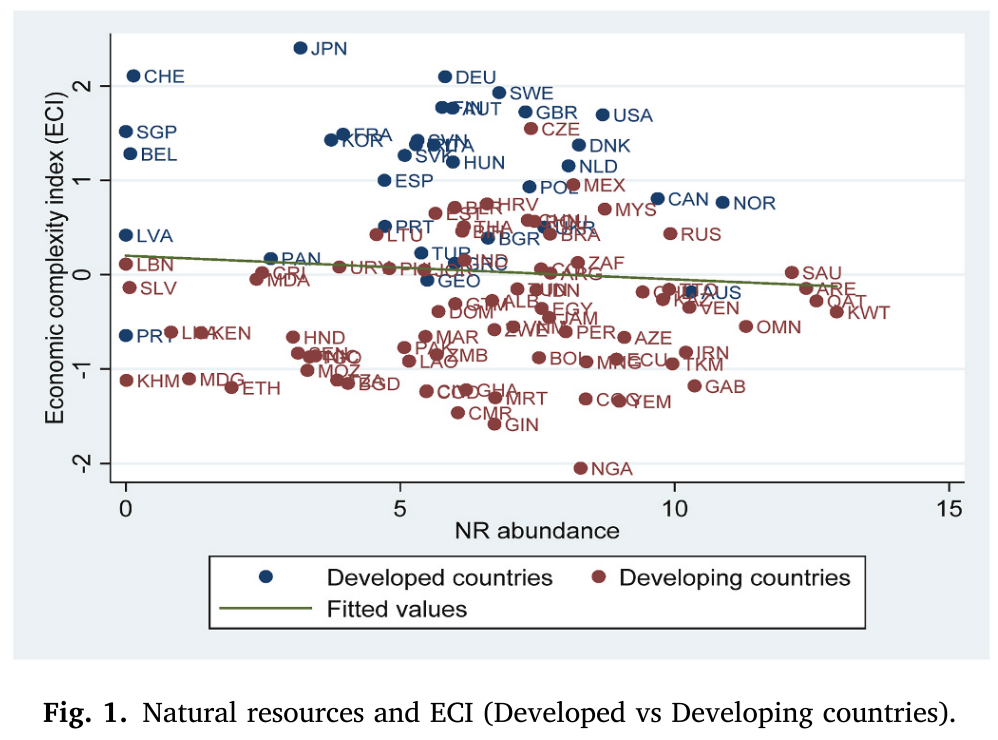
\includegraphics[width=0.85\textwidth]{figures/1_avom_2022.png}
		\caption{
			Abundancia de recursos naturales y complejidad económica (ECI) en países desarrollados y en desarrollo.
		}
		\label{fig:anexo_nr_eci}
		
		\vspace{0.3cm}
		\footnotesize{Fuente: Tomado de Hausmann et al. (2014).}
	\end{figure}
	
	La Figura~\ref{fig:anexo_nr_eci_finance} ilustra la relación entre dependencia de recursos, complejidad económica y niveles de desarrollo financiero, mostrando diferencias sistemáticas según el grado de desarrollo financiero.
	
	\begin{figure}[H]
		\centering
		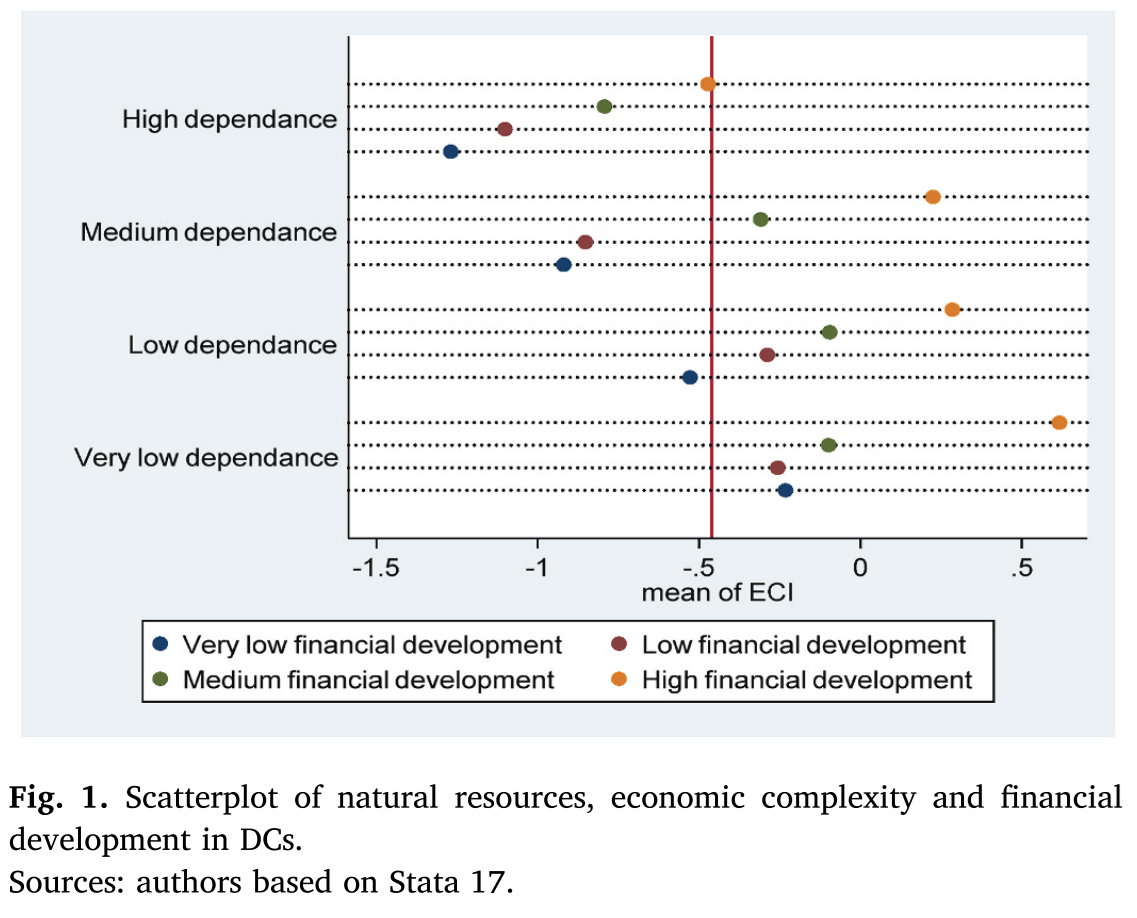
\includegraphics[width=0.85\textwidth]{figures/1_valentine_2024.png}
		\caption{
			Recursos naturales, complejidad económica (ECI) y desarrollo financiero en países en desarrollo.
		}
		\label{fig:anexo_nr_eci_finance}
		
		\vspace{0.3cm}
		\footnotesize{Fuente: Tomado de Valentine et al. (2024).}
	\end{figure}
	
	\section{Mapas}
	\label{sec:mapas}
	
	La \autoref{fig:resource-dependent-map} presenta la distribución geográfica preliminar de los países potencialmente incluidos en la muestra empírica.
	
	\begin{figure}[htbp]
		\centering
		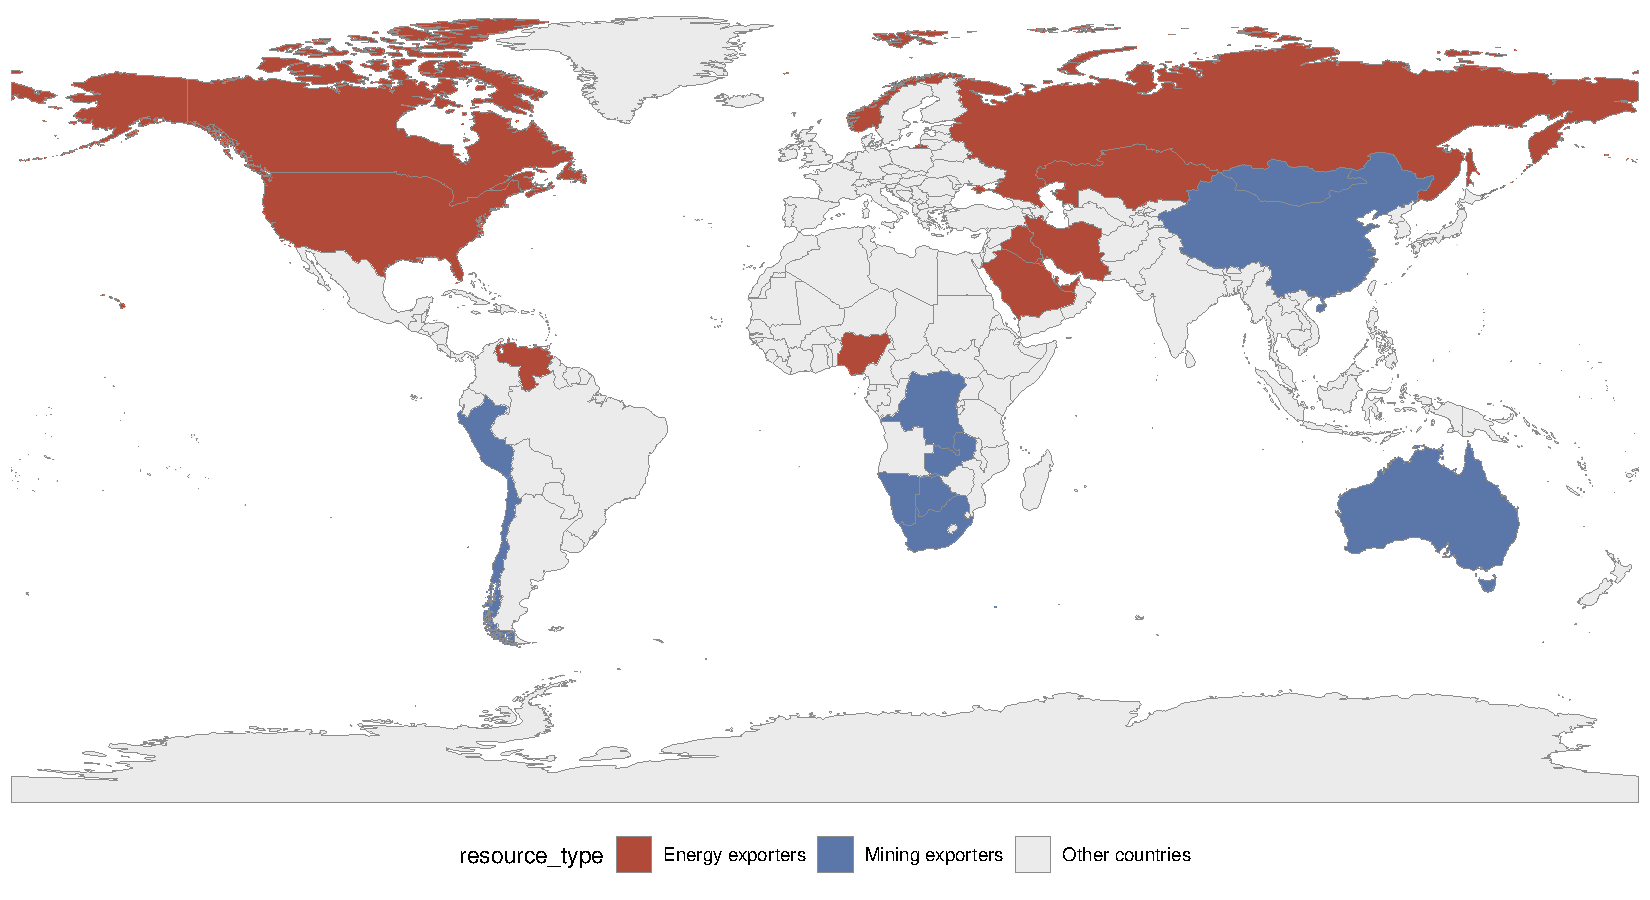
\includegraphics[width=\textwidth]{figures/resource_dependent_map}
		
		\caption[Distribución geográfica de economías dependientes de recursos]{Distribución geográfica de las economías potencialmente dependientes de recursos naturales incluidas en la muestra de análisis.}
		
		\label{fig:resource-dependent-map}
	\end{figure}
	
	La \autoref{fig:resource-rents-world-map} muestra la distribución global de las rentas de recursos naturales como porcentaje del PIB.
	
	\begin{figure}[H]
		\centering
		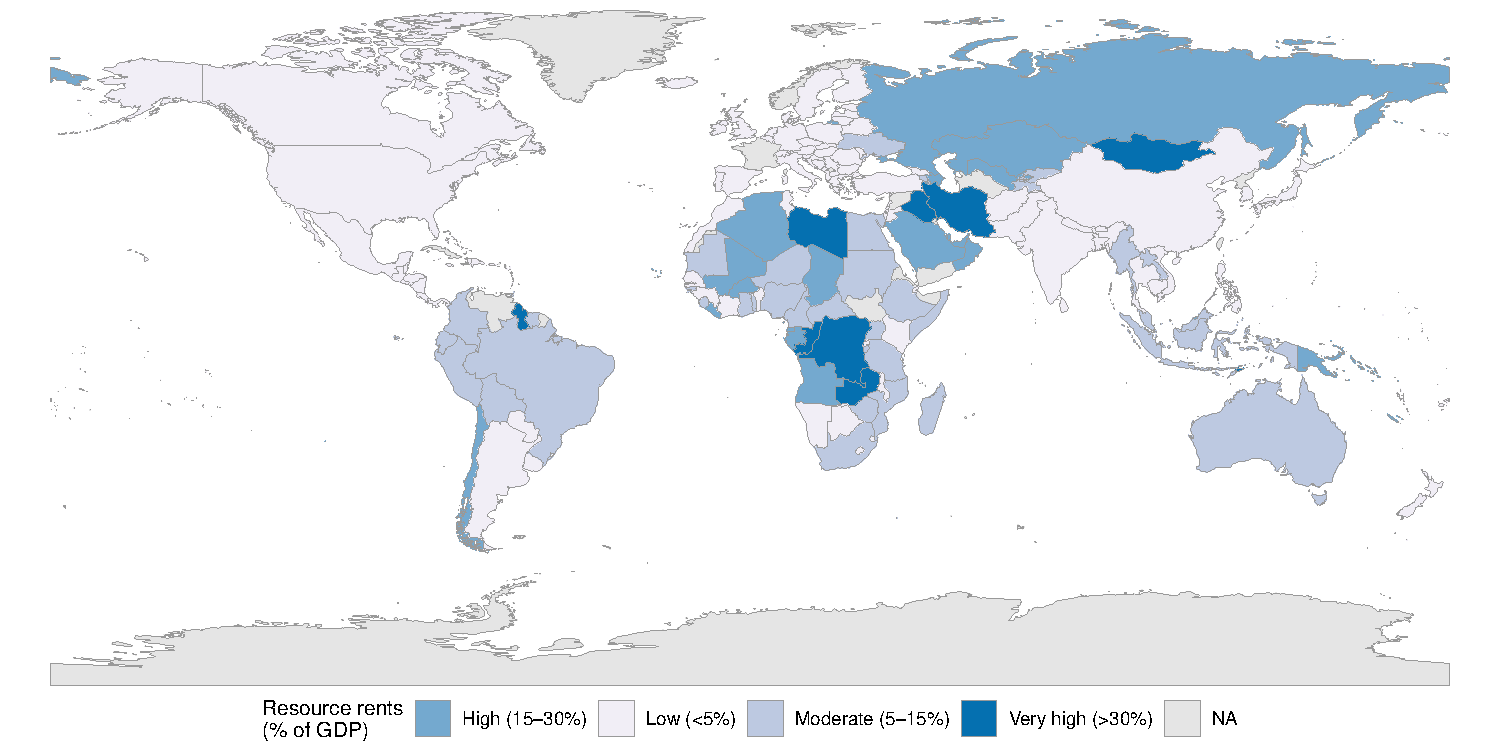
\includegraphics[width=\textwidth]{figures/resource_rents_world_map}
		
		\caption[Rentas de recursos naturales (\% del PIB)]{Distribución global de las rentas de recursos naturales como porcentaje del PIB.}
		
		\label{fig:resource-rents-world-map}
	\end{figure}
	
	La \autoref{fig:eci-world-map} presenta la distribución global del Índice de Complejidad Económica (ECI), un indicador que captura el grado de sofisticación productiva de las economías a partir de la diversidad y ubicuidad de los bienes que exportan. En general, valores más altos del ECI se asocian con estructuras productivas más diversificadas y mayores capacidades tecnológicas, mientras que valores bajos reflejan economías más concentradas en productos primarios o de menor intensidad tecnológica; en este contexto, el mapa ofrece un marco descriptivo para observar las diferencias en capacidades productivas entre países y su posible relación con la dependencia de recursos naturales.
	
	\begin{figure}[H]
		\centering
		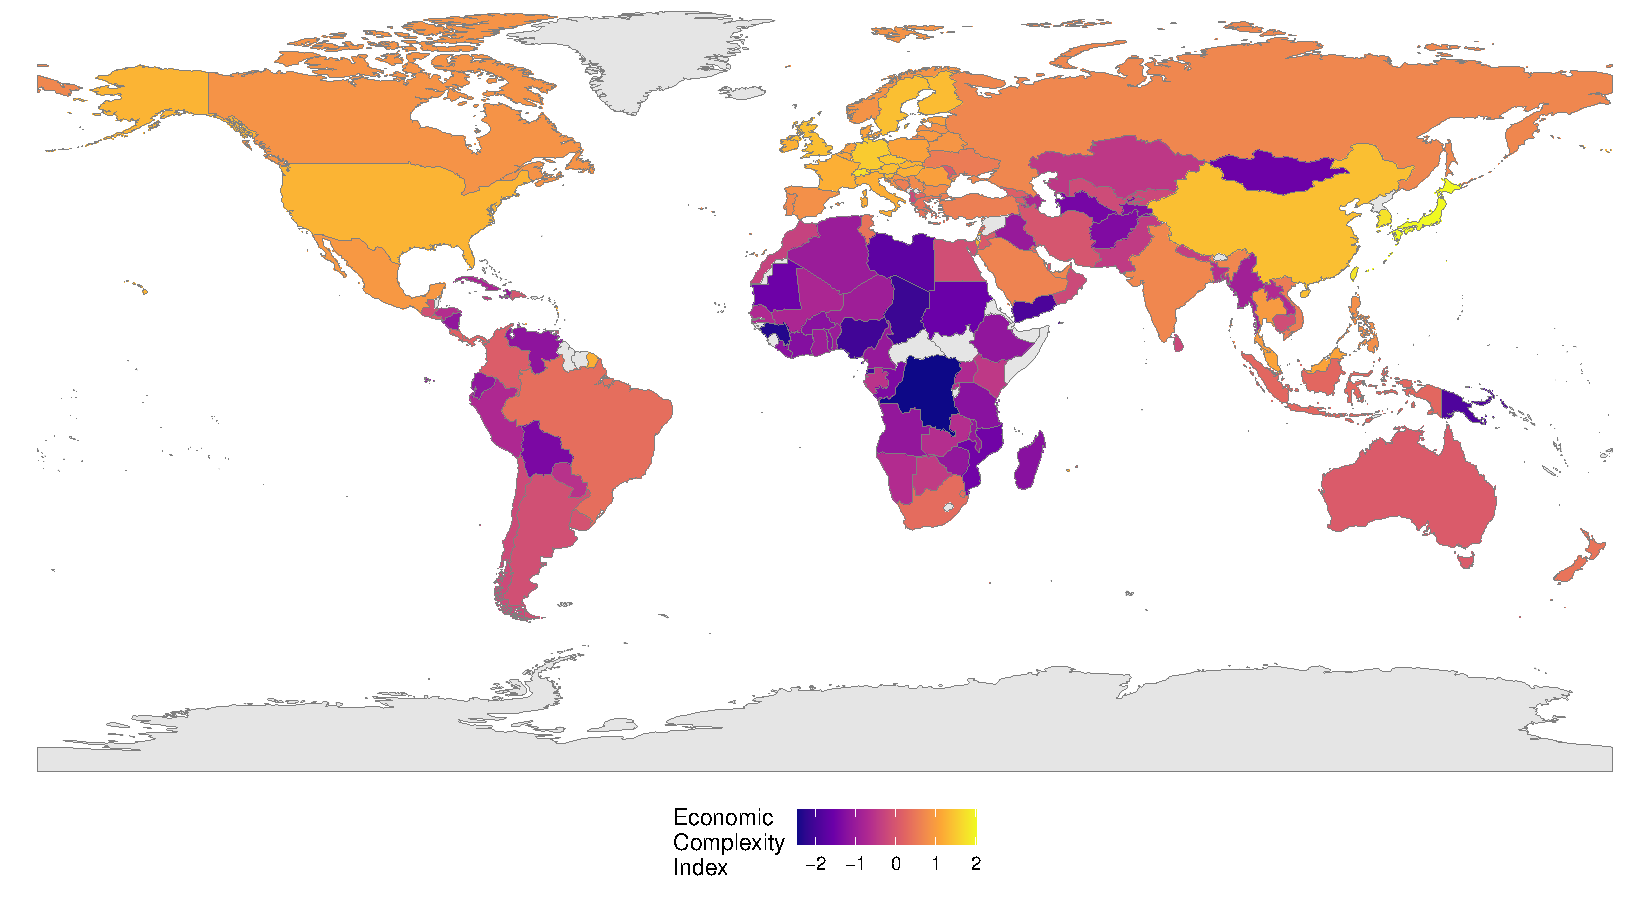
\includegraphics[width=\textwidth]{figures/eci_world_map}
		
		\caption[Distribución global del ECI]{Distribución global del Índice de Complejidad Económica (ECI).}
		
		\label{fig:eci-world-map}
	\end{figure}
	
	La \autoref{fig:eci-world-map-quartiles} muestra la distribución global del Índice de Complejidad Económica (ECI) clasificada por cuartiles. Esta representación permite comparar de manera relativa el nivel de sofisticación productiva entre economías, agrupando a los países según su posición en la distribución mundial del indicador. En particular, el primer cuartil (Q1) corresponde a economías con menor complejidad económica, mientras que el cuarto cuartil (Q4) agrupa a las economías con estructuras productivas más diversificadas y tecnológicamente avanzadas.
	
	\begin{figure}[H]
		\centering
		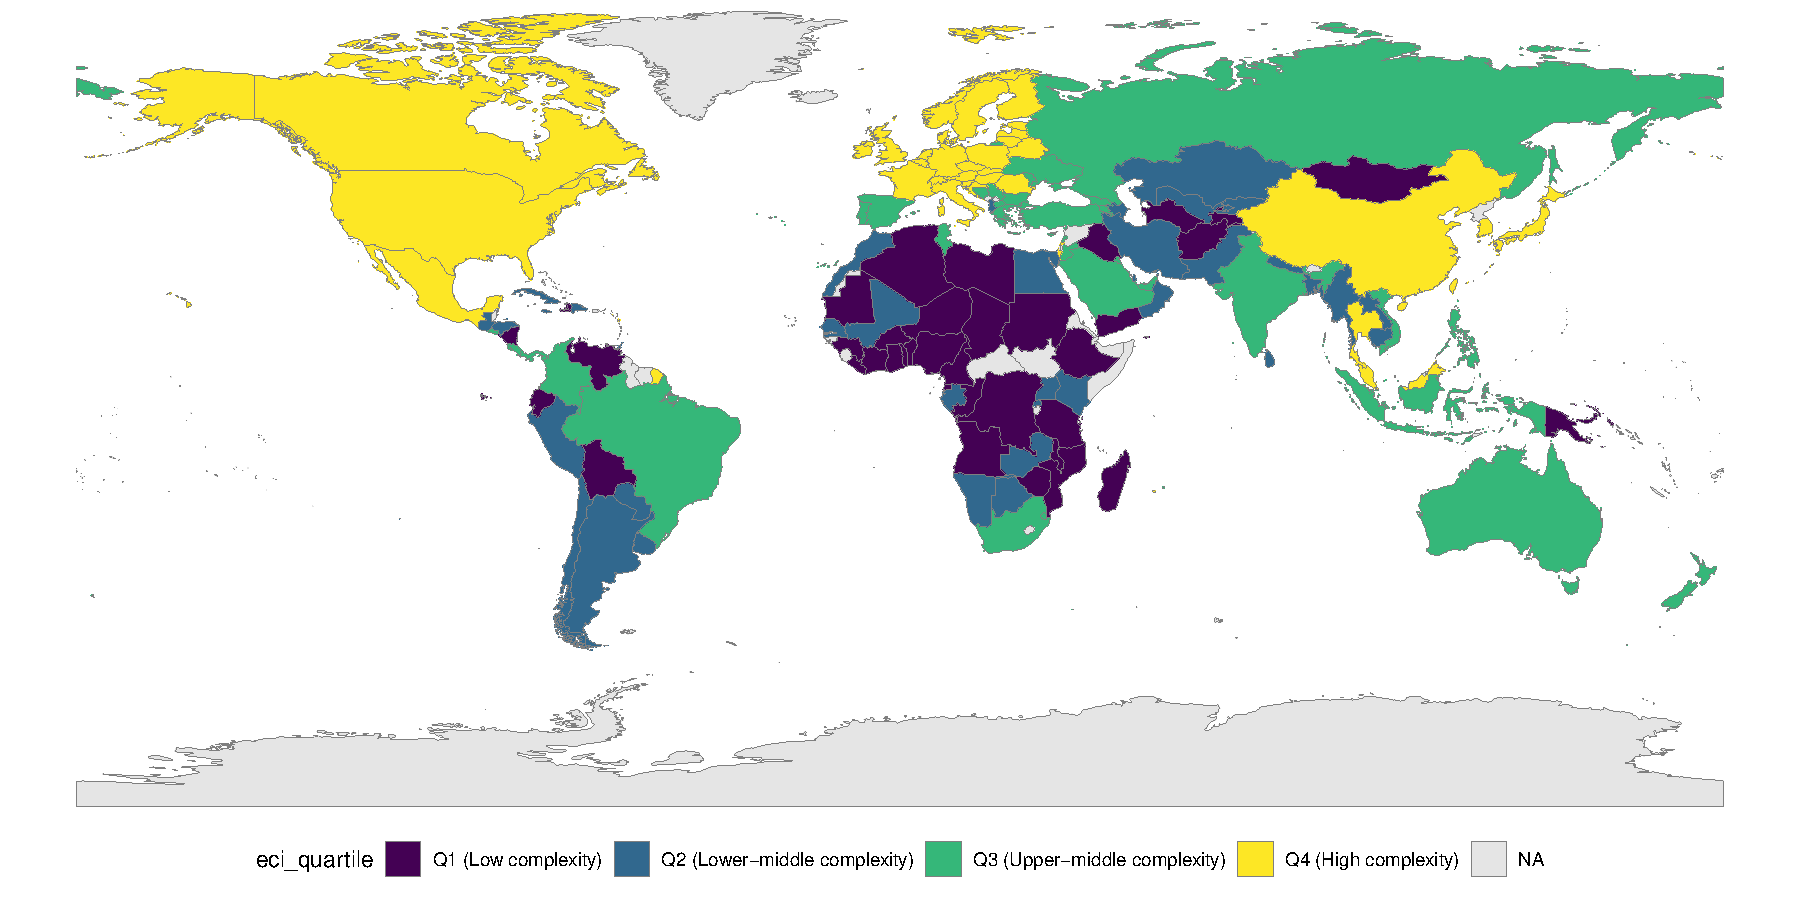
\includegraphics[width=\textwidth]{figures/eci_world_map_quartiles}
		
		\caption[ECI por cuartiles]{Distribución global del Índice de Complejidad Económica (ECI) por cuartiles.}
		
		\label{fig:eci-world-map-quartiles}
	\end{figure}
	
	
	Una representación particularmente ilustrativa de la estructura productiva mundial es el denominado \textit{Product Space}, desarrollado por \textcite{Hausmann2014}. Esta red conecta productos de acuerdo con la proximidad productiva entre ellos, definida a partir de la probabilidad de que dos bienes sean exportados conjuntamente por los mismos países. La visualización resultante revela una topología altamente estructurada en la que los bienes primarios y commodities tienden a ubicarse en la periferia de la red, mientras que las manufacturas complejas —como maquinaria, productos químicos y electrónica— ocupan el núcleo densamente interconectado. Esta estructura sugiere que el desarrollo económico puede entenderse como un proceso de acumulación gradual de capacidades productivas que permite a los países desplazarse desde actividades periféricas hacia sectores más centrales y complejos dentro del espacio productivo.
	
	\begin{figure}[H]
		\centering
		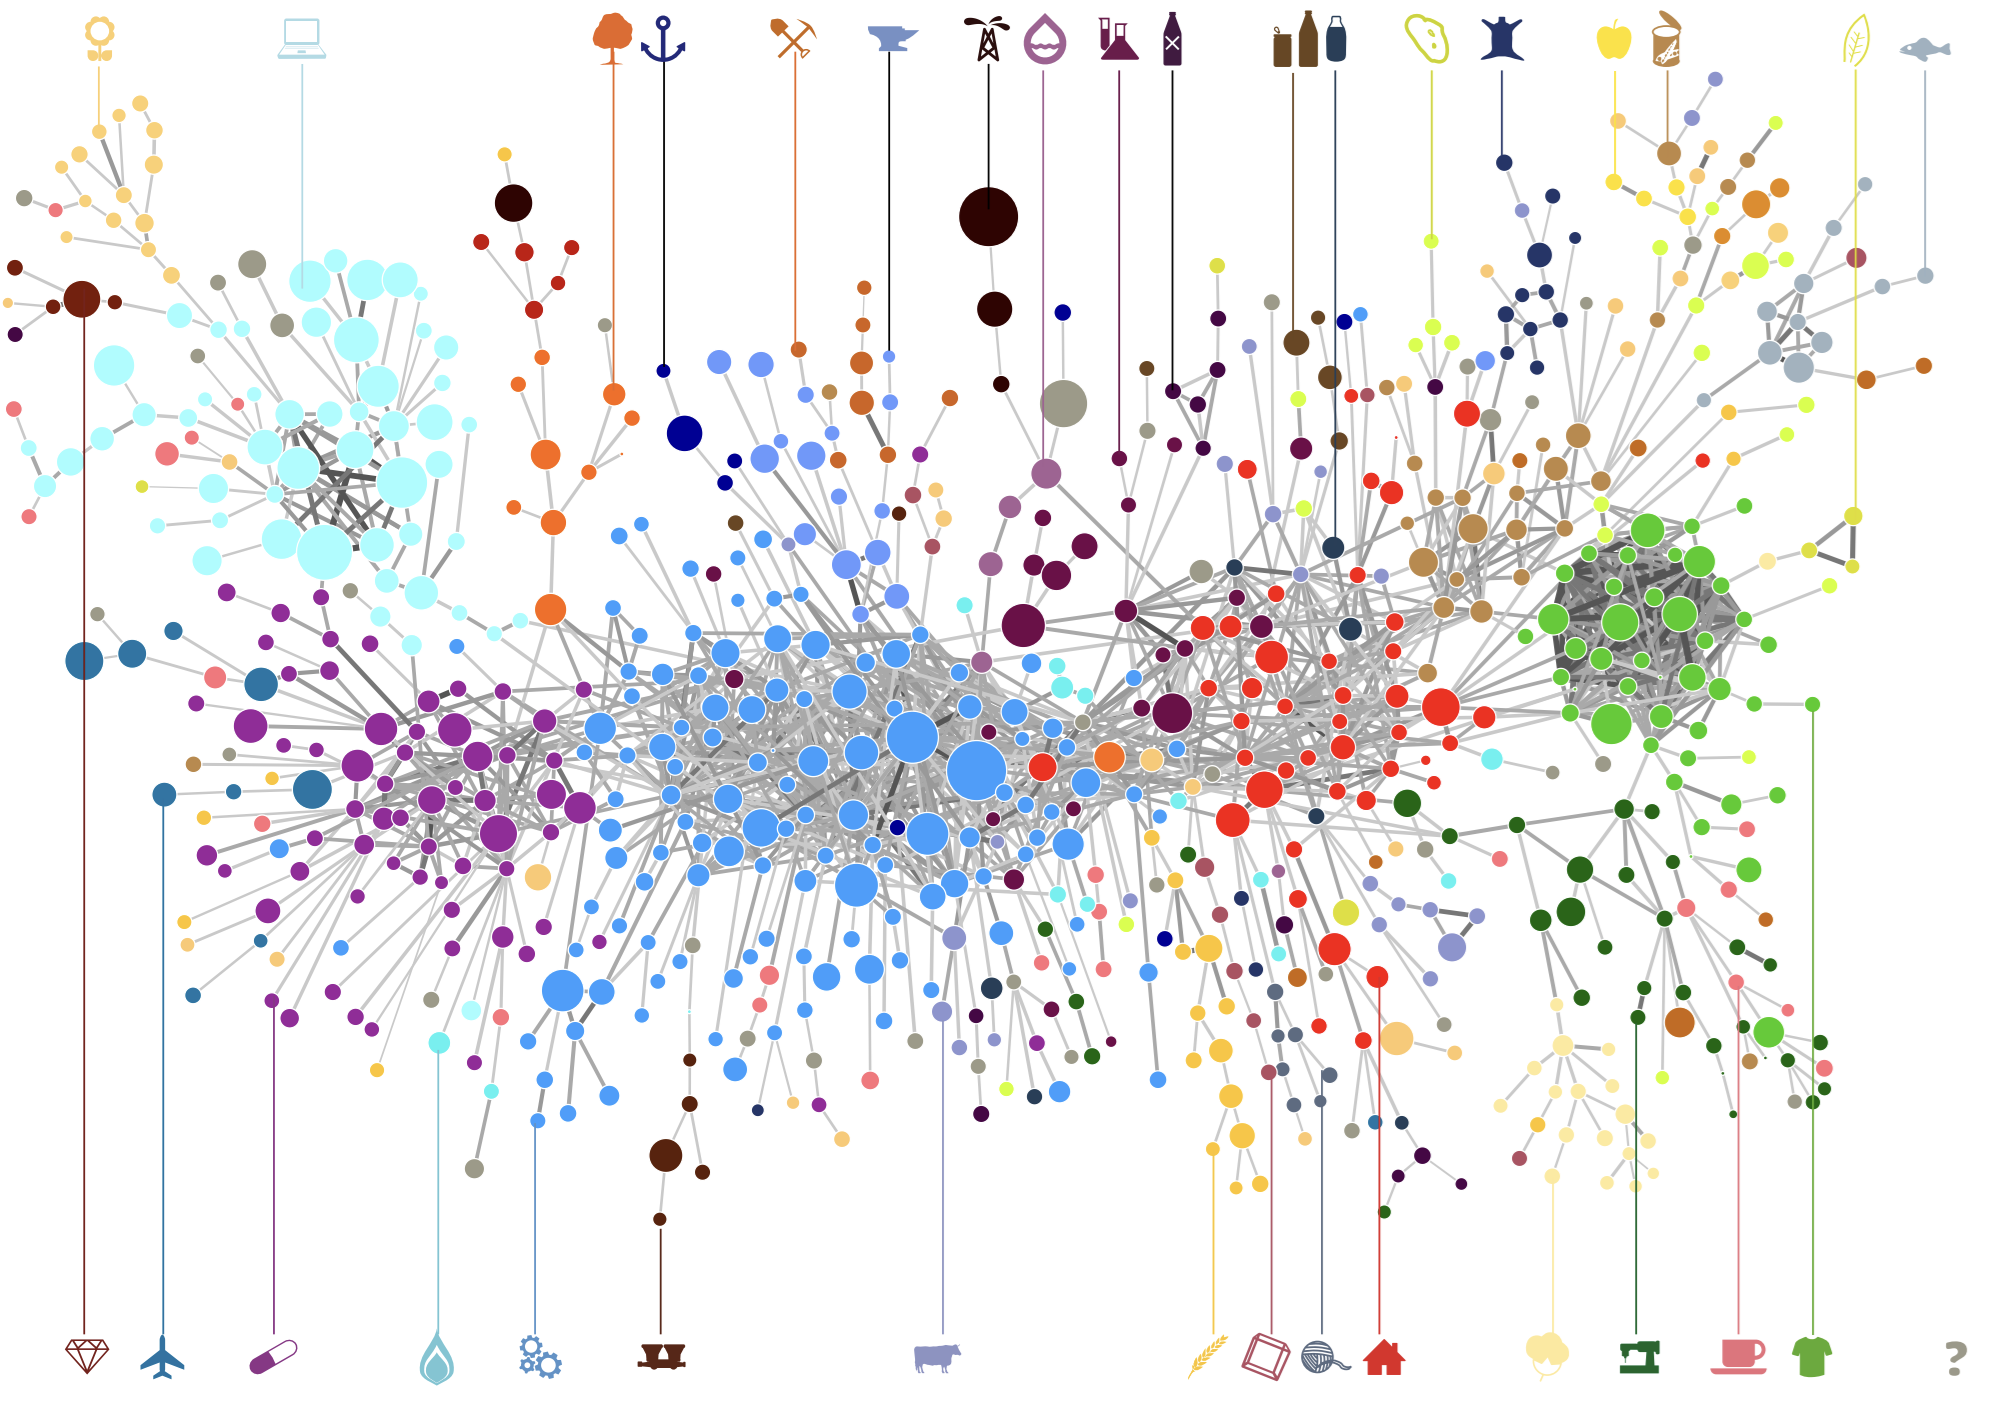
\includegraphics[width=0.95\textwidth]{figures/3_hausmann_2014.png}
		
		\caption[El Product Space]{El \textit{Product Space}: red global de proximidad entre productos basada en patrones de coexportación entre países. Los nodos representan productos y los enlaces reflejan proximidad productiva.}
		
		\label{fig:product_space_hausmann}
		\footnotesize
		Fuente: Adaptado de \textcite{Hausmann2014}.
	\end{figure}
	
	La literatura sobre la \textit{Dutch disease} ha señalado que los auges en los sectores de recursos naturales pueden generar apreciaciones del tipo de cambio real, reasignación de factores productivos y pérdida de competitividad en sectores transables, particularmente en la manufactura \parencite{Barder2006}. Desde la perspectiva del \textit{Product Space} propuesto por \textcite{Hausmann2014}, este fenómeno puede interpretarse como un desplazamiento estructural de la economía hacia regiones periféricas del espacio productivo. En dicho espacio, las actividades de manufactura —especialmente aquellas asociadas a productos más sofisticados— tienden a ubicarse en el núcleo densamente interconectado de la red, debido a la gran cantidad de capacidades productivas compartidas que requieren. En contraste, los bienes primarios y extractivos suelen localizarse en la periferia, caracterizada por un menor número de conexiones con otras actividades productivas. En este sentido, una especialización excesiva en recursos naturales no solo debilita la base manufacturera de la economía, sino que también reduce las oportunidades cercanas para diversificación hacia productos más complejos. En consecuencia, la \textit{Dutch disease} no solo tiene implicaciones macroeconómicas de corto plazo, sino que también puede afectar la trayectoria de acumulación de capacidades productivas, limitando la capacidad de la economía para transitar hacia sectores de manufactura ubicados en el núcleo del espacio productivo.
	
	Como referencia visual al marco analítico desarrollado en esta tesis, la \autoref{fig:product_space_communities} ilustra la estructura del espacio productivo. Esta representación resulta particularmente relevante para el argumento central del presente estudio, ya que muestra cómo distintos grupos de productos se ubican en posiciones heterogéneas en términos de complejidad económica y conectividad productiva. En este contexto, los sectores asociados a manufacturas y bienes industriales tienden a concentrarse en regiones más densamente conectadas del espacio productivo, mientras que muchas actividades primarias y extractivas aparecen en posiciones más periféricas. Esta configuración sugiere que las economías especializadas en recursos naturales pueden enfrentar mayores restricciones estructurales para diversificar hacia actividades de mayor complejidad.
	
	\begin{figure}[H]
		\centering
		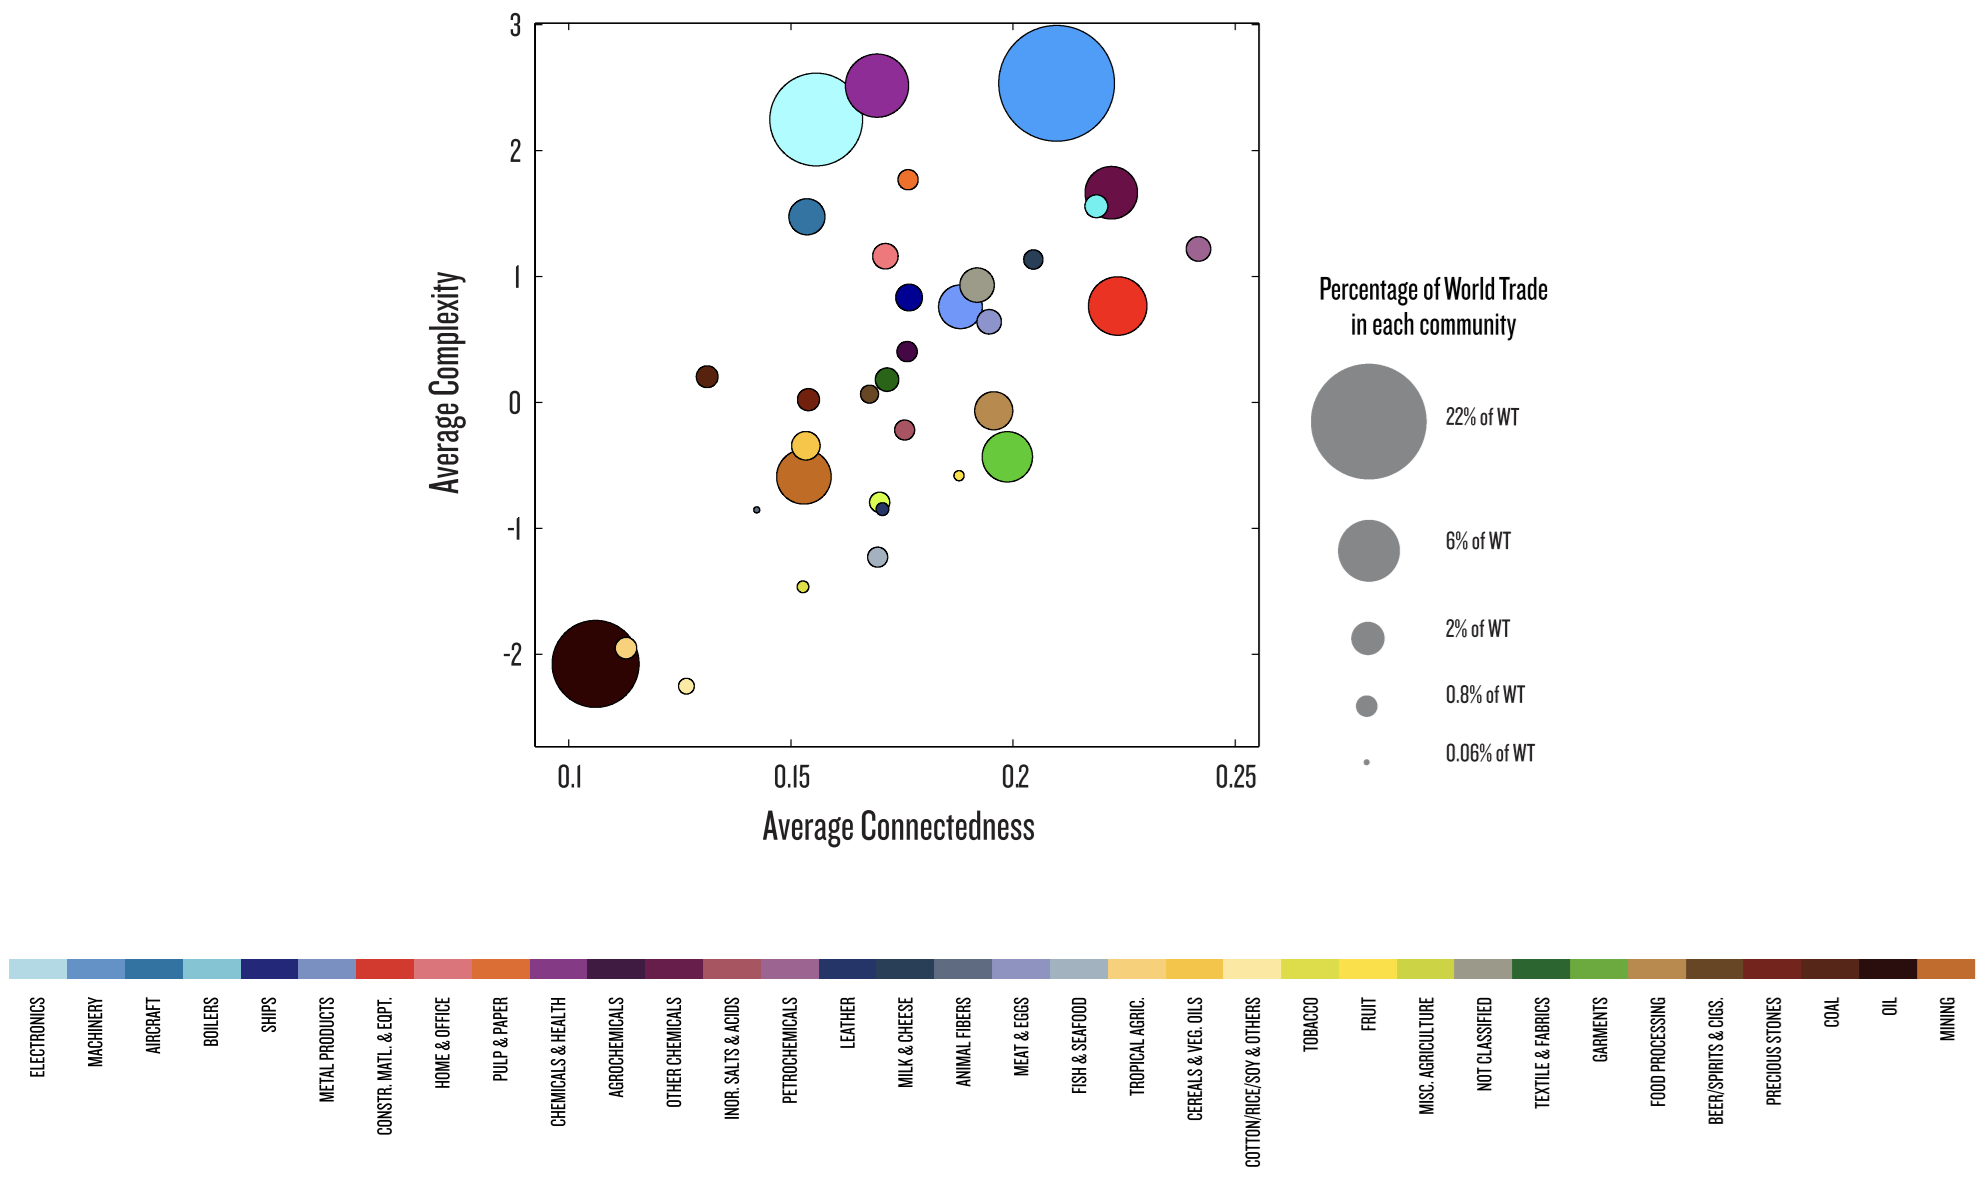
\includegraphics[width=0.9\textwidth]{figures/4_hausmann_2014.png}
		
		\caption[Complejidad y conectividad en el Product Space]{Complejidad promedio y conectividad de comunidades de productos en el espacio productivo global. El tamaño de las burbujas es proporcional a la participación de cada comunidad en el comercio mundial.}
		
		\label{fig:product_space_communities}
		
		\vspace{0.2cm}
		\footnotesize
		\textit{Fuente: Adaptado de} \textcite{Hausmann2014}, \textit{The Atlas of Economic Complexity}.
	\end{figure}
	
	Como se observa en la Tabla \ref{tab:product_communities_selected}, las comunidades asociadas a industrias extractivas presentan valores sustancialmente menores del \textit{Product Complexity Index} (PCI) en comparación con sectores manufactureros intensivos en conocimiento. Este contraste refleja diferencias estructurales en las capacidades productivas requeridas por cada tipo de actividad y resulta consistente con la literatura sobre complejidad económica y diversificación productiva \parencite{Hausmann2014}.
	
	\begin{table}[H]
		\centering
		\caption[Comunidades de productos y complejidad (PCI)]{
			Características seleccionadas de comunidades de productos en el espacio productivo, incluyendo complejidad promedio (PCI), número de productos y participación en el comercio mundial.
		}
		\label{tab:product_communities_selected}
		
		\begin{threeparttable}
			\begin{tabular}{lcccc}
				\toprule
				\textbf{Community} & \textbf{Average PCI} & \textbf{Number of Products} & \textbf{World Trade} & \textbf{World Share} \\
				\midrule
				\multicolumn{5}{l}{\textit{Extractive industries}} \\
				
				Oil & -2.08 & 4 & 2.3T & 10.49\% \\
				Mining & -0.59 & 48 & 1.1T & 5.01\% \\
				Coal & 0.21 & 6 & 183B & 0.83\% \\
				
				\midrule
				\multicolumn{5}{l}{\textit{Manufacturing sectors (contrast)}} \\
				
				Machinery & 2.54 & 125 & 4.4T & 20.29\% \\
				Electronics & 2.25 & 52 & 3.6T & 16.71\% \\
				Chemicals \& Health & 2.52 & 64 & 1.6T & 7.47\% \\
				
				\bottomrule
			\end{tabular}
			
			\begin{tablenotes}
				\footnotesize
				\item \textit{Fuente: elaboración propia a partir de datos reportados en} \textcite{Hausmann2014}, \textit{The Atlas of Economic Complexity}.
			\end{tablenotes}
			
		\end{threeparttable}
	\end{table}
	
	
	Las visualizaciones del espacio productivo pueden explorarse de forma interactiva en el \textit{Atlas of Economic Complexity} desarrollado por el Harvard Growth Lab \citeyear{HarvardGrowthLab2024}
	
	\section{Tablas descriptivas sobre dependencia de recursos naturales}
	\label{sec:tablas}
	
	Las economías dependientes de recursos naturales no constituyen un grupo homogéneo. Estas difieren tanto en su nivel de desarrollo económico como en el tipo de sector extractivo dominante. En particular, algunos países presentan una fuerte especialización en exportaciones energéticas (petróleo y gas), mientras que otros se especializan principalmente en minerales, o bien presentan estructuras extractivas mixtas. La Tabla \ref{tab:extractive_typology} presenta una tipología estilizada que clasifica las economías dependientes de recursos según el tipo de sector extractivo predominante y su nivel de ingreso, siguiendo la clasificación de ingresos del Banco Mundial.
	
	\begin{table}[H]
		\centering
		\caption[Tipología de economías extractivas]{Tipología de economías dependientes de recursos naturales según tipo de sector extractivo y nivel de ingreso.}
		\label{tab:extractive_typology}
		
		\begin{threeparttable}
			\begin{adjustbox}{max width=\textwidth}
				\begin{tabular}{lcccc}
					\toprule
					\textbf{Tipo de economía extractiva} & \textbf{LIC} & \textbf{LMIC} & \textbf{UMIC} & \textbf{HIC} \\
					& (Low Income) & (Lower Middle) & (Upper Middle) & (High Income) \\
					\midrule
					
					\textbf{Economías energéticas} \\
					(Energy $\gg$ Mining)
					& Chad, Sudan
					& Nigeria
					& Azerbaijan
					& Norway \\
					
					\addlinespace
					
					\textbf{Economías mineras} \\
					(Mining $\gg$ Energy)
					& DR Congo
					& Guinea, Zambia
					& Mongolia, Peru, Kazakhstan
					& Chile, Australia \\
					
					\addlinespace
					
					\textbf{Economías extractivas mixtas} \\
					(Mining + Energy)
					& 
					& Mauritania
					& Indonesia, Colombia
					& Russia, Canada \\
					
					\bottomrule
				\end{tabular}
			\end{adjustbox}
			
			\begin{tablenotes}[para,flushleft]
				\footnotesize
				\item \textit{Nota: LIC = Low Income Countries; LMIC = Lower Middle Income Countries; UMIC = Upper Middle Income Countries; HIC = High Income Countries. La clasificación por ingreso sigue la tipología vigente del Banco Mundial (FY2026). Venezuela, RB, aparece actualmente sin clasificar por falta de datos comparables y por ello no se incluye en la tabla.}
			\end{tablenotes}
		\end{threeparttable}
	\end{table}

	\thesisendchap{anexos}
	
\end{document}
